%%%%%%%%%%%%%%%%%%%%%%%%%%%%%%%%%%%%%%%%%
% Thin Sectioned Essay
% LaTeX Template
% Version 1.0 (3/8/11)
%
% This template has been downloaded from:
% http://www.LaTeXTemplates.com
%
% Original Author:
% Nicolas Diaz (nsdiaz@uc.cl) with extensive modifications by:
% Vel (vel@latextemplates.com)
%
% License:
% CC BY-NC-SA 3.0 (http://creativecommons.org/licenses/by-nc-sa/3.0/)
%
%%%%%%%%%%%%%%%%%%%%%%%%%%%%%%%%%%%%%%%%%

%----------------------------------------------------------------------------------------
%	PACKAGES AND OTHER DOCUMENT CONFIGURATIONS
%----------------------------------------------------------------------------------------

\documentclass[a4paper, 11pt]{article} % Font size (can be 10pt, 11pt or 12pt) and paper size (remove a4paper for US letter paper)

\usepackage[protrusion=true,expansion=true]{microtype} % Better typography
\usepackage{graphicx} % Required for including pictures
\usepackage{wrapfig} % Allows in-line images

\usepackage{mathpazo} % Use the Palatino font
\usepackage[T1]{fontenc} % Required for accented characters
\linespread{1.05} % Change line spacing here, Palatino benefits from a slight increase by default

\makeatletter
\renewcommand\@biblabel[1]{\textbf{#1.}} % Change the square brackets for each bibliography item from '[1]' to '1.'
\renewcommand{\@listI}{\itemsep=0pt} % Reduce the space between items in the itemize and enumerate environments and the bibliography

\renewcommand{\maketitle}{ % Customize the title - do not edit title and author name here, see the TITLE block below
\begin{flushleft} % Right align
{\LARGE\@title} % Increase the font size of the title

\vspace{50pt} % Some vertical space between the title and author name

{\large\@author} % Author name
\\\@date % Date

\vspace{40pt} % Some vertical space between the author block and abstract
\end{flushleft}
}

%----------------------------------------------------------------------------------------
%	TITLE
%----------------------------------------------------------------------------------------

\title{\textbf{NIKA2 research note}\\   
\textsc{NIKA2 Commissioning results v1.0}} % Subtitle


\author{NIKA2 team % Author
\\{\textit{NIKA2 collaboration}}} % Institution

\date{\today} % Date



%----------------------------------------------------------------------------------------

\begin{document}

\maketitle % Print the title section
\tableofcontents
%----------------------------------------------------------------------------------------
%	ABSTRACT AND KEYWORDS
%----------------------------------------------------------------------------------------

%\renewcommand{\abstractname}{Summary} % Uncomment to change the name of the abstract to something else

\begin{abstract}
This notes describe the main results of the NIKA2 commissioning campaigns.
\end{abstract}

%\hspace*{3,6mm}\textit{Version:}  % Version

\vspace{30pt} % Some vertical space between the abstract and first section

%----------------------------------------------------------------------------------------
%
%	ESSAY BODY
%
%----------------------------------------------------------------------------------------
%\tableofcontents


%----------------------------------------------------------------------------------------
%	INRODUCTION
%----------------------------------------------------------------------------------------
\section{Introduction}

\subsection{Commissioning goals}
The main goal of the NIKA2 commissioning runs described below is to check the performance of the instrument and its stability with respect to the specifications described in Table \ref{nika2specs}.

%\begin{table}[h]
%\caption{Commissioning campaigns and dates}
%\label{nika2specs}
%\begin{tabular}{|c|c|c|s}
%\hline 
% FWHM &   &  \\
%\hline  
%\hline 
%\end{tabular} 
%\end{table} 



\subsection{Commissioning runs}
We had 10 commissioning runs for NIKA2 as described in Table~\ref{nika2runs}.

\begin{table}[h]
\small
\caption{Commissioning campaigns, dates and general comments.
\label{nika2runs}}
\begin{tabular}{|c|c|c|c|c|}
\hline 
RUN  & NIKA Run & Starting date    & End date         &  General comments \\
\hline
N2R1     & 13       & 29-October-2015   & 10-November-2015 & Not full instrumentation        \\
N2R2     & 14       & 24-November-2015  & 02-December-2015 & 13 NIKEL boards working         \\
N2R3     & 15       & 12-January-2016   & 01-February-2016 & 20 NIKEL boards                 \\
N2R4     & 16       & 1-March-2016      & 15-March-2016    & 	                               \\
Dark run & 17       & 4-May-2016        & 4-May-2016       & Dark tests with N2R4 conditions  \\
\hline
N2R5     & 18       & 16-September-2016 & 11-October-2016  & New dichroic, corrugated lenses, \\
         &          &                   &                  &  new array 2 mm, new electronics \\
N2R6     & 19       & 25-October-2016   & 1-November-2016  &                                  \\
N2R7     & 20       & 6-December-2016   & 13-December-2016 & Test external calibrator         \\
N2R8     & 21       & 9-January-2017    & 13-January-2017  & Replace array 1 lens by smooth one \\
         &          & 24-January-2017   & 25-January-2017  & Tests on the sky   \\
N2R9     & 22       & 21-February-2017  & 28-February-2017 &                                   \\
N2R10    & 23       & 18-April-2017     & 25-April-2017    & End of commisioning phase 1,     \\
         &          &                   &                  & Science verification  \\  
\hline
\end{tabular} 
\end{table} 


%----------------------------------------------------------------------------------------
%	BANDPASSES
%----------------------------------------------------------------------------------------
\section{Bandpasses}
\begin{figure}[ht] % Inline image example
\begin{center}
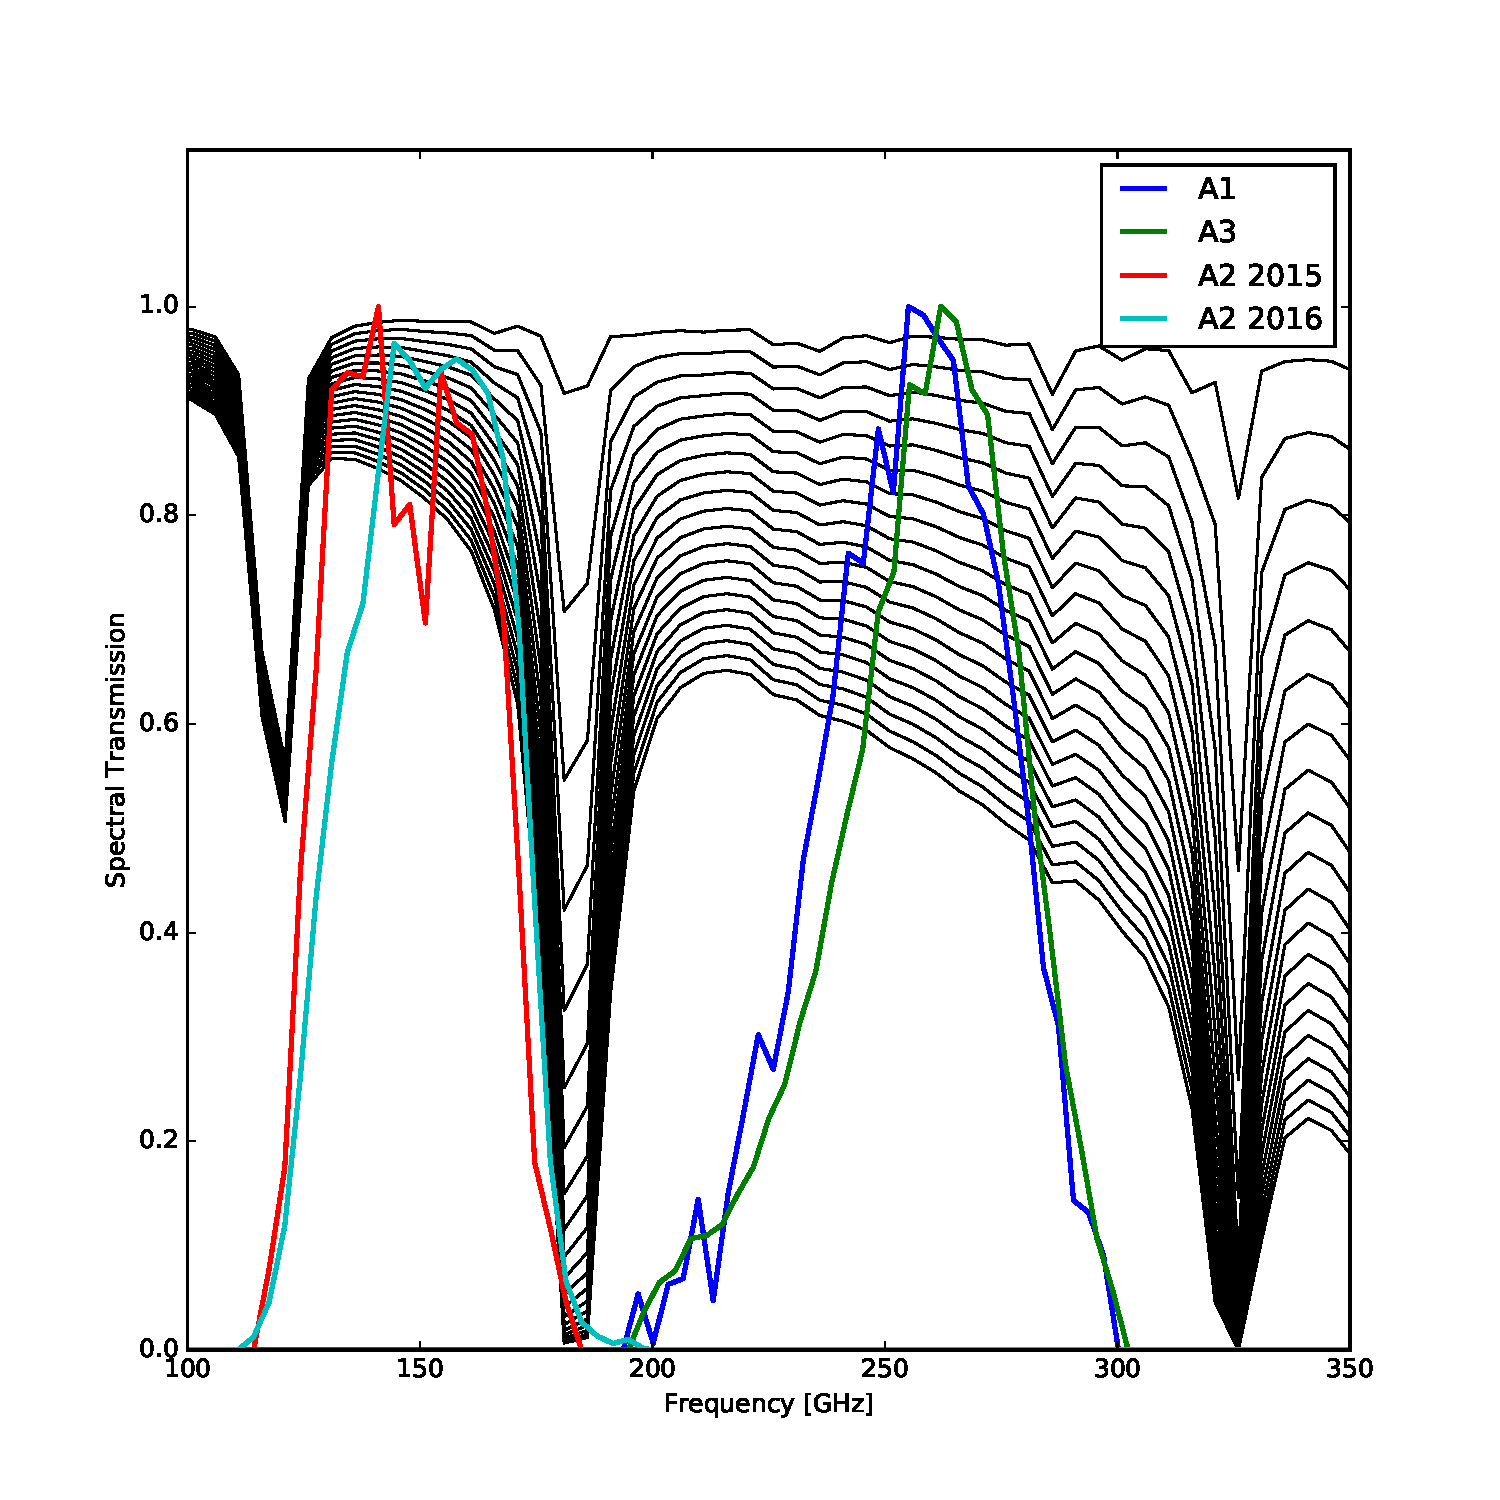
\includegraphics[width=\textwidth]{Figures/SpectralBands/atm_transmission.pdf}
\end{center}
\caption{Spectral transmission of the the three NIKA2 arrays as a function of frequency in GHz. For illustration we also plot the ATM atmospheric model for different values of pwv. \label{spectralband}}
\end{figure}




The NIKA2 spectral bands were measured in the laboratory using a Martin Pupplet interferometer.
Both arrays and filter bands were considered in the measurements. Theser were obtained from the difference of two black-bodies, hence they include a a $\nu^2$ RJ term. During the commissioning in Run 5 array 2 was replaced. The new array has a different spectral transmission. Figure shows the spectral transmissions for the three arrays. Notice that array A2 was replaced by a new on in N2R5 and that the spectral transmissions are not the same (red and cyan lines in the figure).


\begin{table}[h]
\caption{Spectral transmission characteristics for the NIKA2 arrays.%
\label{nika2runs}}
\begin{tabular}{|c|c|c|c|c|}
\hline 
  &     A1  &  A3 &  A2 2015 & A2 2016 \\ 
\hline 
Central Frequency [GHz] &   255.5  & 257.8   &   147.7  & 151.6 \\  
Bandwidth [GHz]         &   47.8   & 45,7    &   41.8   & 42.1 \\
\hline 
\end{tabular} 
\end{table} 


What actually matters more than the ``central frequency'' that depends on many
assumptions and definitions are the bandpasses. We should make available in a
.fits file, clearly, our bandpasses to avoid future misunderstanding and propagation of
false numbers. Official values should be 150 and 260~GHz. We should also clearly
state that these measured bandpasses were done with the difference of two
black-bodies, hence they include a $\nu^2$ RJ term.\\

With these bandpasses and an official ATM spectrum, we expect an opacity ratio of
XX between 1 and 2mm and see~\ref{se:opacities} for more details.





%----------------------------------------------------------------------------------------
%	OPACITY
%----------------------------------------------------------------------------------------
\section{Opacity derivation}
\label{se:opacities}

For each kid $k$, $f_{tone}^k$ moves with the atmospheric load according to

\begin{equation}
f_{tone}^k = C_0^k + C_1^k T_{atm}[1-e^{-\tau/\sin\delta}]
\end{equation}

where $\delta$ is the elevation. The {\tt skydip} procedure consists in moving
the telescope in elevation step by step and to monitor, for each kid, the
evolution of $f_{tone}^k$ vs the air mass and to fit the opacity $\tau$ and
$C_0^k$ and $C_1^k$. All the skydips (that were obtained under various opacity
conditions) are analysed together to break the degeneracies between these
parameters. The procedure has two steps. First, all the skydips are analysed
individually to simply measure $f_{tone}^k$ for each stable elevation and fit
simultaneously all the parameters. Error bars on $\tau$ are estimated by doing
this procedure on blocks of 40 kids only and getting a dispersion on the
resulting $\tau$ from the different blocks. Usually the dispersion comes out as
$4\times 10^{-3}$ at 1mm and $1\times 10^{-3}$ at 2mm. Once the $\tau$ values
are estimated for each skydip (as the average over the blocks), we compute
(while fixing $\tau$) the $C_0$ and $C_1$ final values for each kid. We thus
retrieve the coefficients of all the Kids even though some of them could not
contribute to the tau determination.

%% \begin{figure}
%% \begin{center}
%% 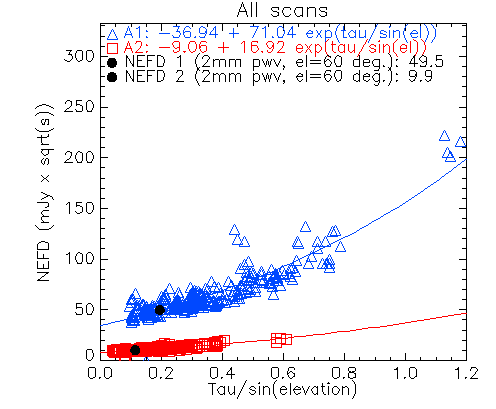
\includegraphics[clip, angle=0, scale =
%%   0.5]{Figures/NEFD_vs_tau_20170226s415_FXDC0C1_Jy_common_mode_kids_out.png}
%% 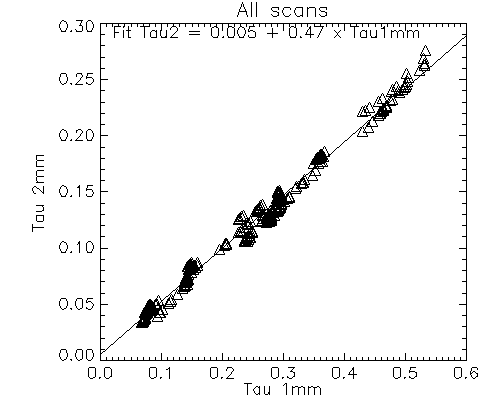
\includegraphics[clip, angle=0, scale =
%%   0.5]{Figures/tau1_tau2_20170226s415_FXDC0C1_GaussPhot_common_mode_kids_out.png}
%% \caption{}
%% \label{fig:fov}
%% \end{center}
%% \end{figure}

\begin{figure}
\begin{center}
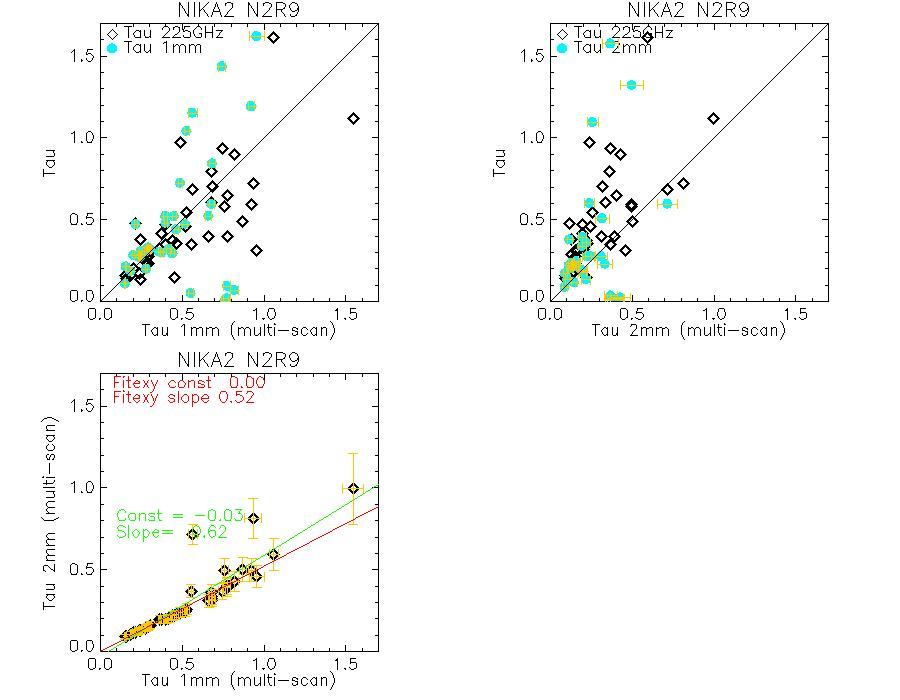
\includegraphics[clip, angle=0, scale = 0.5]{Figures/test_allskd_N2R9.jpg}
\caption{{\bf Fix me : improve plot quality and plot only the 3rd one.}}
\label{fig:test_allskd_N2R9}
\end{center}
\end{figure}


%----------------------------------------------------------------------------------------
%	FOCAL PLANE RECONSTRUCTION
%----------------------------------------------------------------------------------------
\section{Focal plane reconstruction}
\label{se:fov}

\begin{figure}
\begin{center}
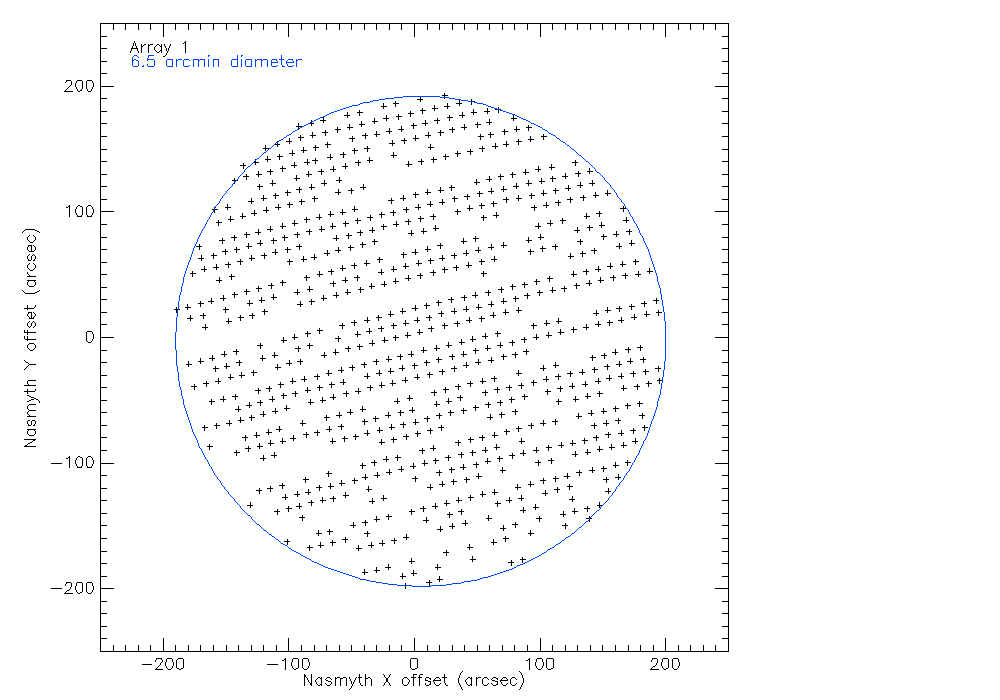
\includegraphics[clip, angle=0, scale = 0.15]{Figures/FOV_A1.png}
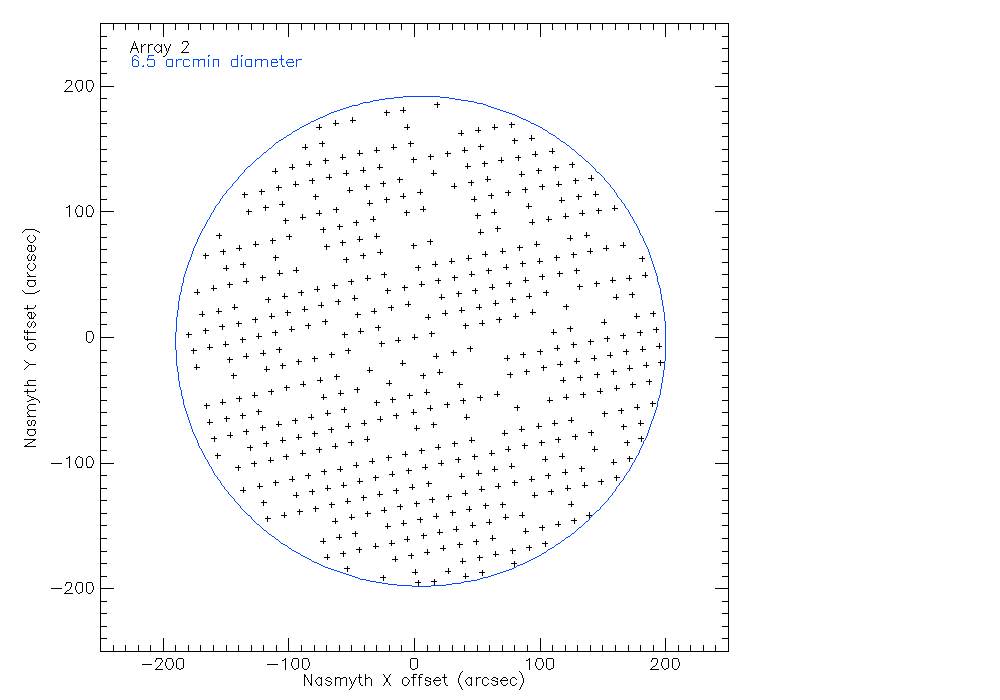
\includegraphics[clip, angle=0, scale = 0.15]{Figures/FOV_A2.png}
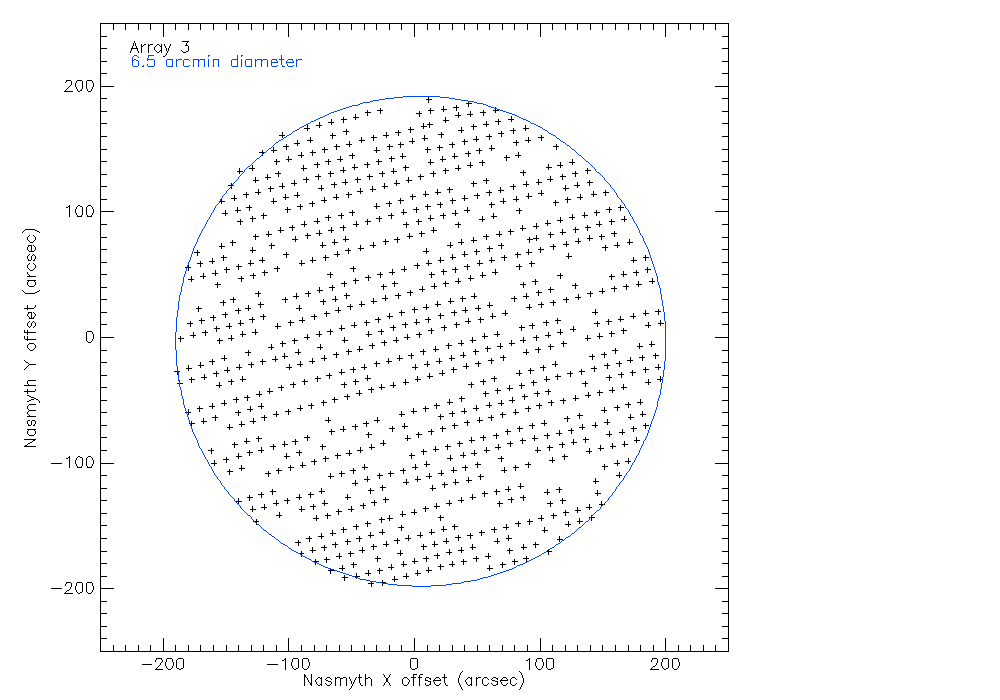
\includegraphics[clip, angle=0, scale = 0.15]{Figures/FOV_A3.png}
\caption{Nasmyth offsets of each array, from beammap 26s415 on 3C84.}
\label{fig:fov}
\end{center}
\end{figure}

\begin{table}
\begin{tabular}{|l|l|l|}
\hline
Array & Number of valid kids & Fraction of all kids\\
\hline
A1 & 793 & 0.75\\
A2 & 481 & 0.83\\
A3 & 872 & 0.83\\
\hline
\end{tabular}
\end{table}

\begin{equation}
FOV diameter = \sqrt{4 N_{tot. kids} * gridstep^2/\pi}
\end{equation}

The same definition applies to ``Effective FOV'' to avoid extra multiplication
by the fraction of valid pixels

\begin{equation}
F\lambda = gridstep\times D(30m)/\lambda
\end{equation}


%----------------------------------------------------------------------------------------
%	POINTING
%----------------------------------------------------------------------------------------
\section{Pointing accuracy}
\label{se:pointing}
% + RTA pointing estimate method
% + pointing model
% + pointing error (scan-to-scan scattering)


%----------------------------------------------------------------------------------------
%	BEAM PATTERN
%----------------------------------------------------------------------------------------
\section{Beam pattern}
\label{se:beams}
%%
%%
%%      SECTION: BEAM PATTERN 
%%

%% [intro]
%%________________________________________________________

The NIKA2 beam pattern mainly depends on the IRAM 30m telescope and NIKA2 internal optical system characteristics, whereas the detectors themselve might have an impact at sub-dominant level (through e.g. time constants or correlated noises). In this section, first we reconstruct the focus surfaces and present the optimal focus, then we characterize both the main beam, which is modeled as an elliptical Gaussian, and the full beam pattern including error beams up to angular scales of 10 arcmin. 

%% [Optimal Focus]
%%________________________________________________________
\subsection{Optimal focus}

\subsubsection{Focus estimation}

[DESCRIPTION NK-OTF-FOCUS + 1 FIG. D'EXEMPLE]

\subsubsection{Reconstruction of the focus surfaces}

[DESCRIPTION BEAMMAP SEQUENCE + FIGS]


%% [Main beam]
%%________________________________________________________
\subsection{Main beam}

For NIKA2 main beam characterization, we use \emph{Run9} OTF scans of bright point sources, including primary and secondary calibrators. Namely, we consider scans of Uranus, Neptune, 3C273, 3C84, 0316+413, Vesta and MWC349, whereas we avoid CRL2688 and NGC7027, which are slighltly extended. We perform a conservative data selection from the observing conditions by demanding average elevations $\rm{el} \ge 20°$, zenith opacities as estimated by NIKA2 in the 1mm band $\tau_{1\rm{mm}} \le 0.4$, reasonable lateral focus settings $x, y \le 0.5$mm. After selection cuts, our data set includes 130 OTF scans, which consists of a representative sub-sample of a typical NIKA2 observation campaign.    

  
We consider different methods for the main beam characterization: i) Gaussian fits of the beam profile to benefit from the signal-over-noise increase after azimuthally averaging the signal, ii) Elliptical Gaussian fits of the beam map for a better 2D modeling. Cross-checking the outputs from these complementary methods is an important robustess test of our results.   


\subsubsection{profile-based analysis}

[JEAN-FRANCOIS]

\subsubsection{map-based analysis}

NIKA2 main beam two-dimensionnal distribution is modeled using an elliptical Gaussian. We characterize NIKA2 resolution by giving the \emph{FWHM}, defined as
\begin{equation}
  FWHM = 2 \sqrt{2\ln {2}} \sqrt{\sigma_x\sigma_y},
\end{equation}
where $\sigma_x$ and $\sigma_y$ are the Gaussian standard deviation along minor- and major-axis. To avoid the side lobes contamination, we use masked versions of the beam map, in which an annulus of inner radius $r_{\rm{in}}$ and outter radius $r_{\rm{out}}$ is cut out. Whereas $r_{\rm{out}}$ is conservately set to be $100 arcsec$, $r_{\rm{in}}$ can vary to provide the best 2D Gaussian fit. We checked a posteriori that $r_{\rm{in}}$ distributes as $7 \pm 1.5$ arcsec at 1mm and $13 \pm 4$ arcsec at 2mm, in agreement with settings defined in the profile-based analysis.   

Figure~\ref{fig:fwhm_map} shows FWHM distributions obtained from the elliptical Gaussian fit method.


\begin{figure}
\begin{center}
  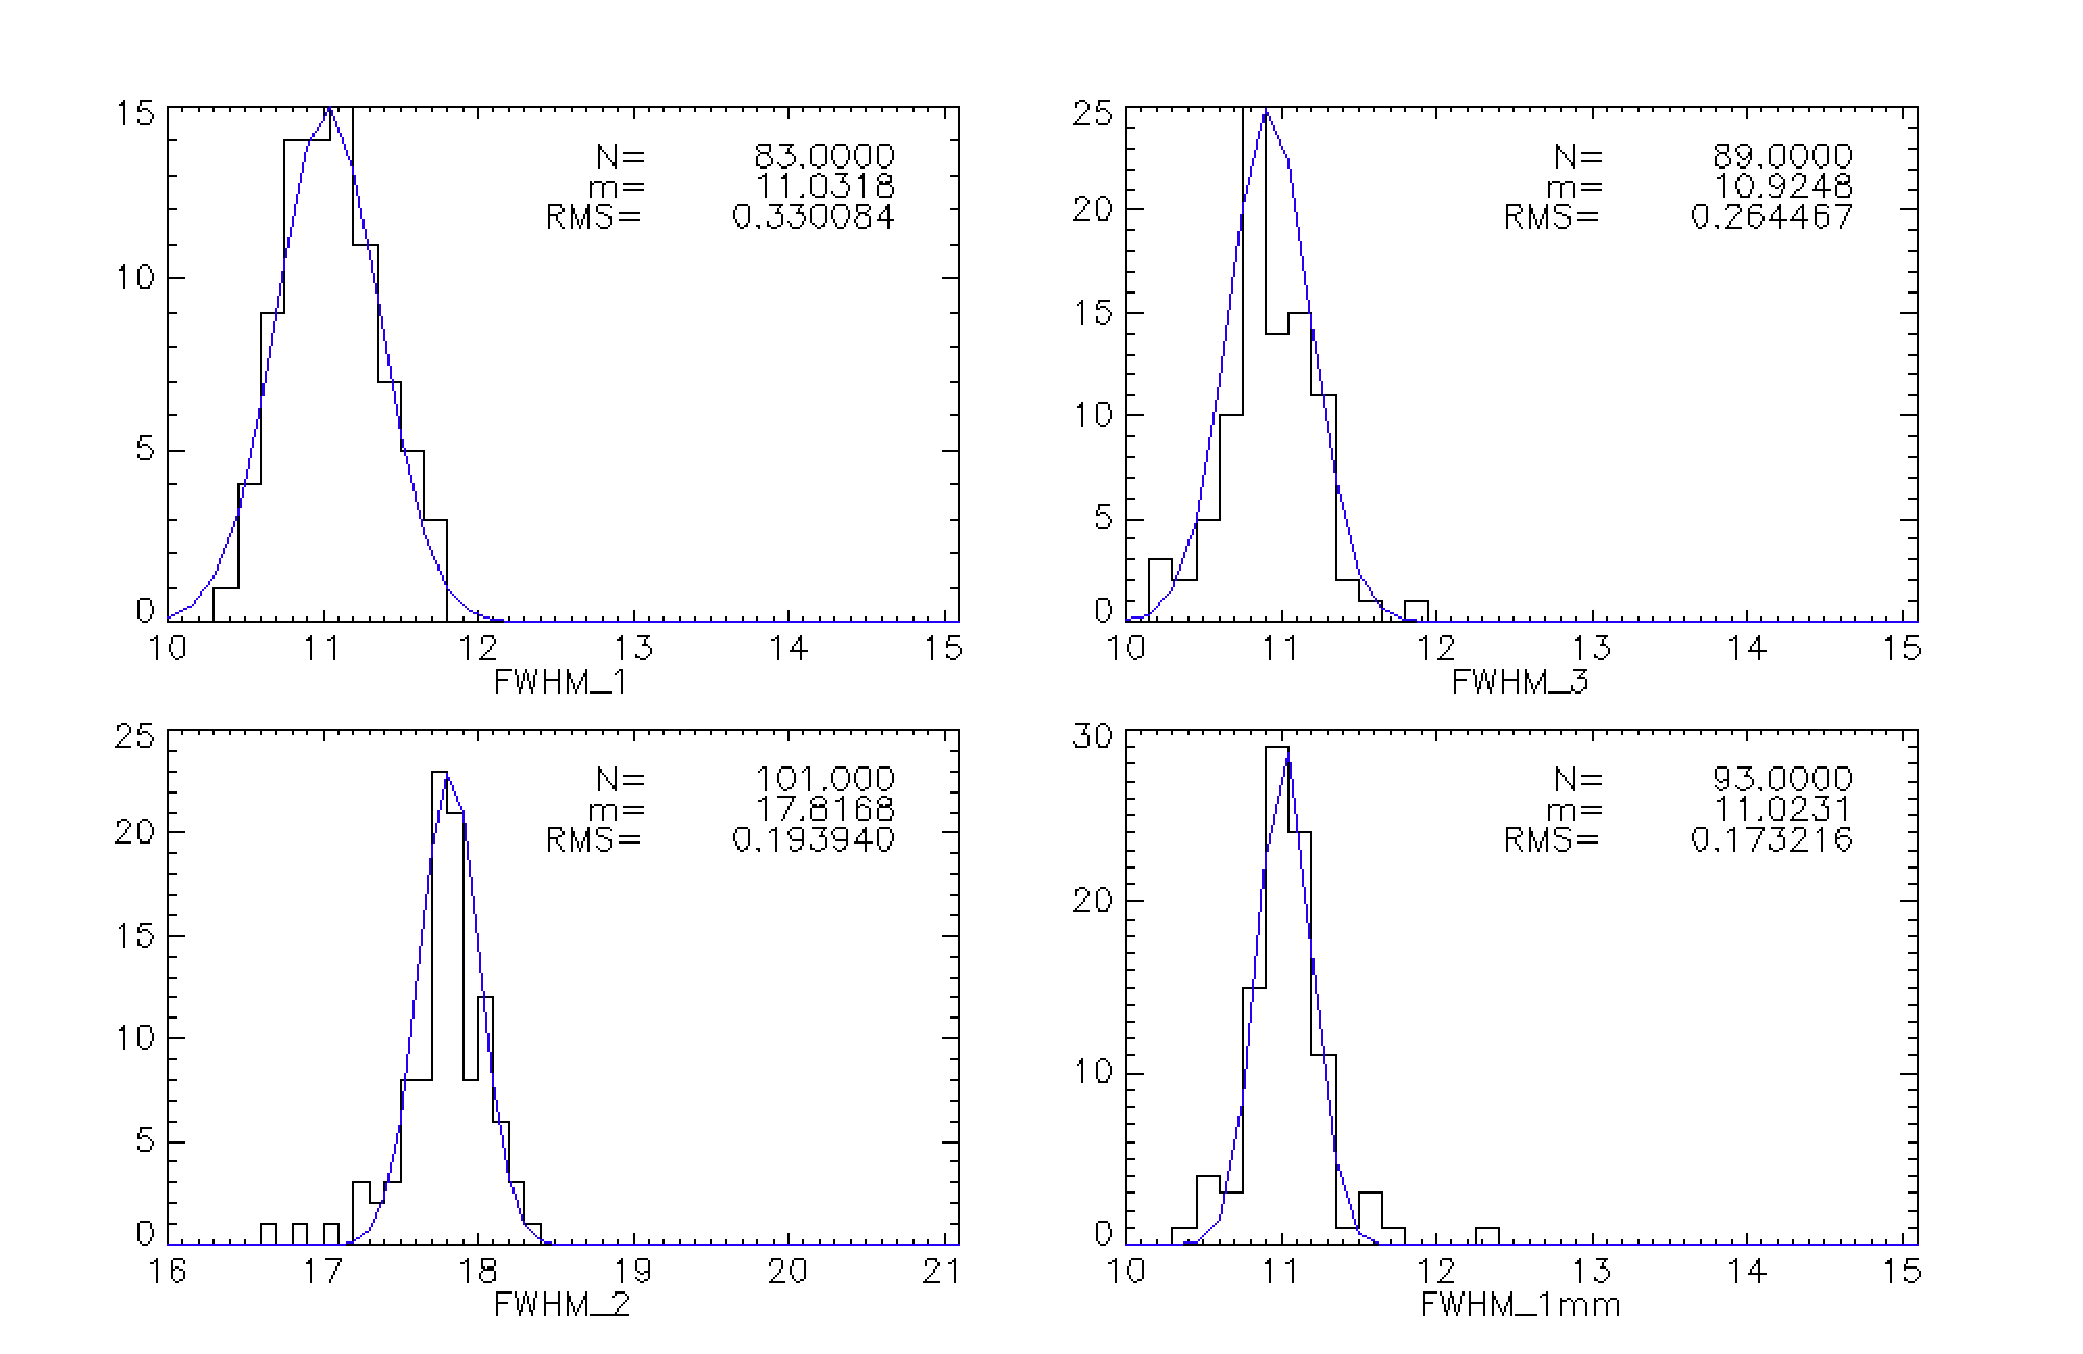
\includegraphics[clip, angle=0, scale=0.4]{Figures/plot_histo_fwhm_run9_calibII_all_nocut.pdf}
\caption{Distribution of the FWHM estimates using 2D Gaussian fits on \emph{N2R9} OTF scans of brigth point sources}
\label{fig:fwhm_map}
\end{center}
\end{figure}


The FWHM estimates using the profile-based and map-based methods are gathered in Tab.~\ref{tab:fwhm}. 
\begin{table}
  \caption[]{FWHM of the NIKA2 main beam in arcsec.}
  \centering
  \begin{tabular}{|l|l|l|l|l|}
    \hline
    Array & profile-based method & map-based method \\
    \hline
    A1       & [TBC] & $11.0 \pm 0.3$ \\
    A3       & [TBC] & $10.9 \pm 0.3$ \\
    A1 \& A3 & [TBC] & $11.0 \pm 0.2$ \\
    A2       & [TBC] & $17.8 \pm 0.2$ \\
    \hline
  \end{tabular}
  \label{tab:fwhm}
\end{table}



%% [Full beam pattern]
%%________________________________________________________
\subsection{Full beam pattern}

\subsubsection{Deep beam maps}
We present the two-dimensional distribution of the beam in Fig.~\ref{fig:beam}. We primary use a map obtained from a combination of deep observations of strong point sources collected during \emph{NIKA2-run8} and \emph{run9}. Namely, we use 'beammap' OTF scans of Uranus (scan id '20170125s223' and '20170125s243'),  Neptune ('20170224s177') and the bright quasar 3C84 ('20170226s415'). However, we checked the stability of our results on single scan maps, combinations of scans for a single source, and combinations of shallower scans but spanning a large range of scanning direction. The data processing includes a mitigation of the correlated noise, which mainly originates from the atmosphere.  We primarly use a subtraction of a common mode estimated from the most correlated detectors (the so-called 'cm one block' method). However, other methods are tested for assessing the immunity of our results to noise residuals.

\begin{figure}
\begin{center}
  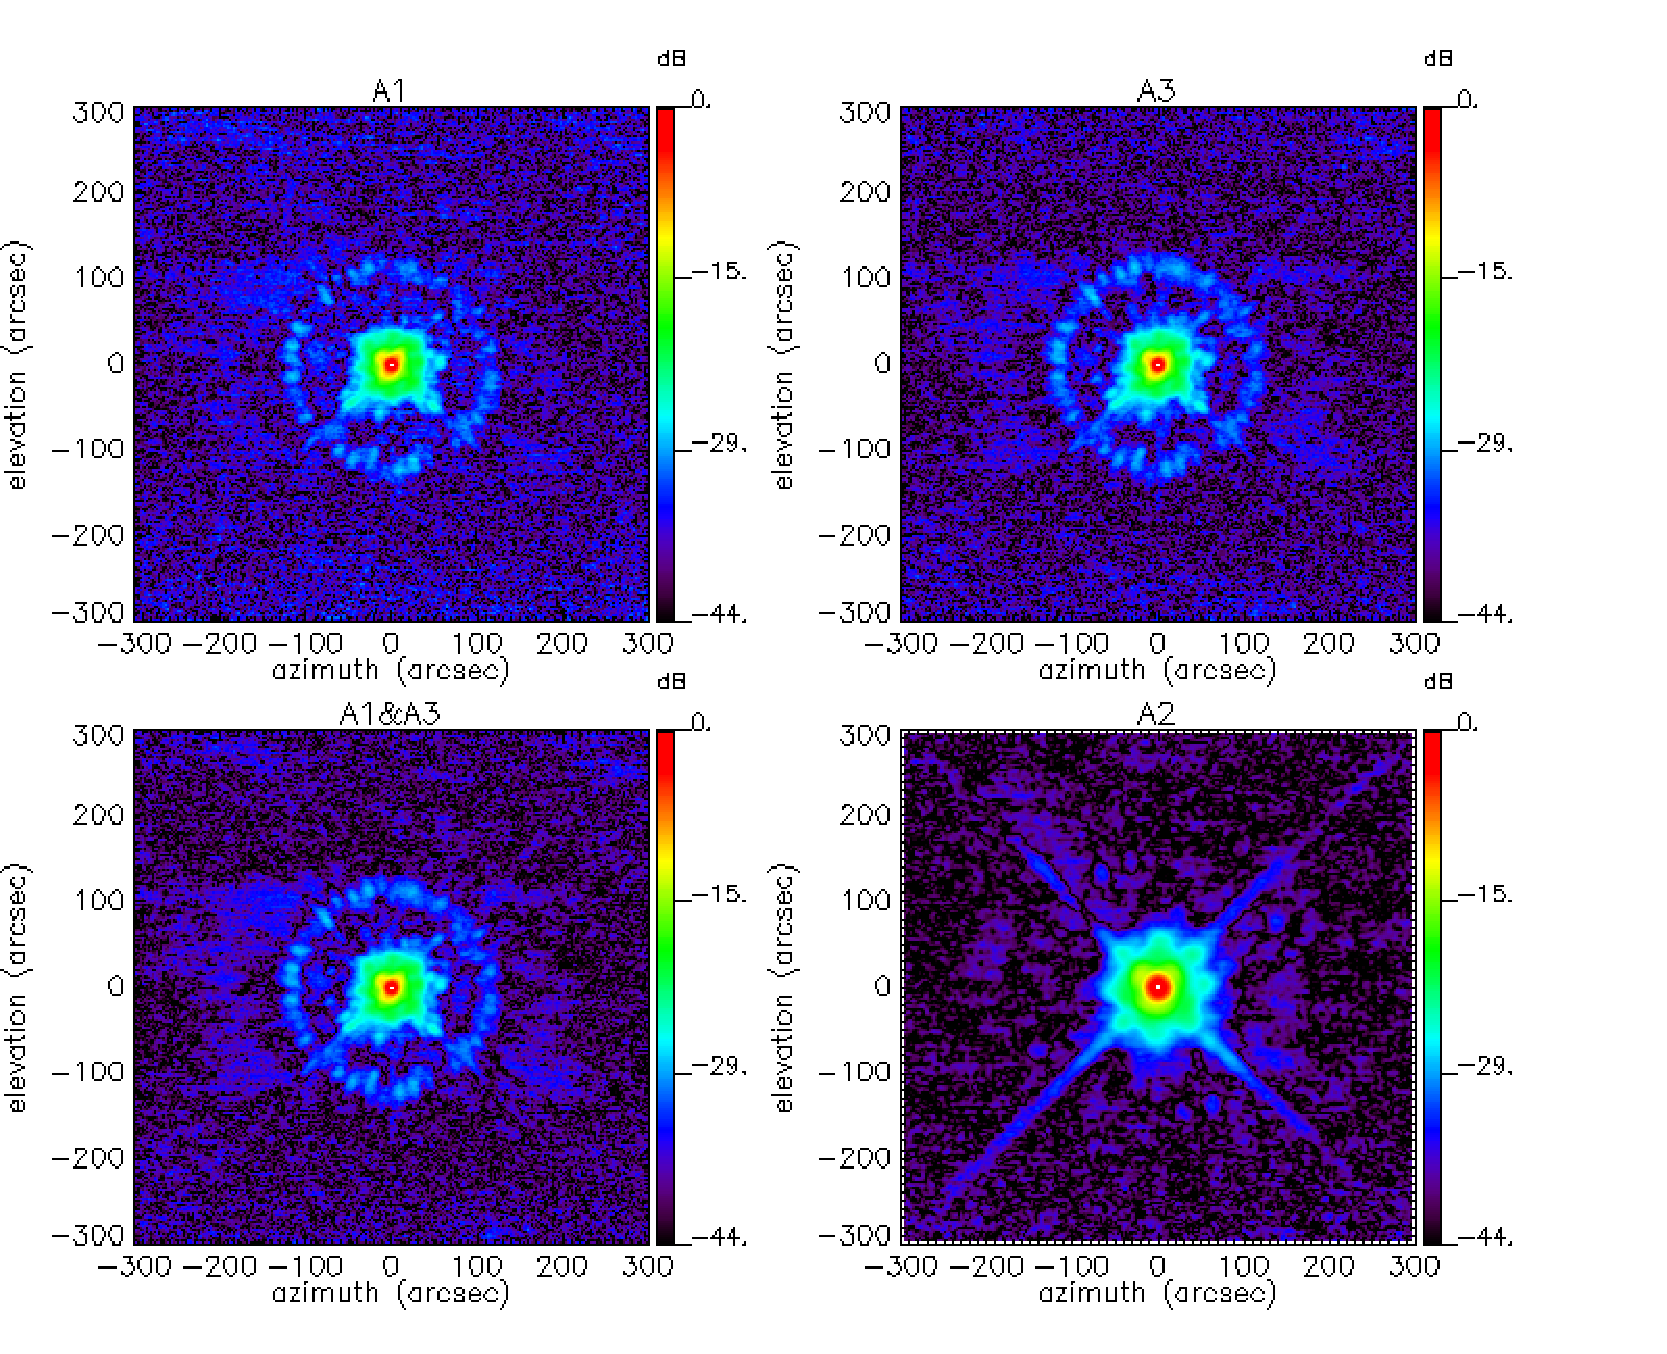
\includegraphics[clip, angle=0, scale=0.4]{Figures/Lobe_map_Combo_v2_dB.pdf}
 \caption{Beam pattern. From upper left to lower right, beam maps of array 1 (labeled 'A1'), array 3 ('A3'), the combination of the 1.15mm arrays ('A1$\&$3') and the 2mm array ('A2') are shown in decibel. These maps, which consist of normalized combination of four long OTF scans of bright point sources, are in celestial coordinates and cover a sky area which extend over 10 arcmin.}
\label{fig:beam}
\end{center}
\end{figure}


The deep NIKA2 beam maps reveal some noticeable features, which are shown in Fig.~\ref{fig:features}. 

\begin{figure}
\begin{center}
  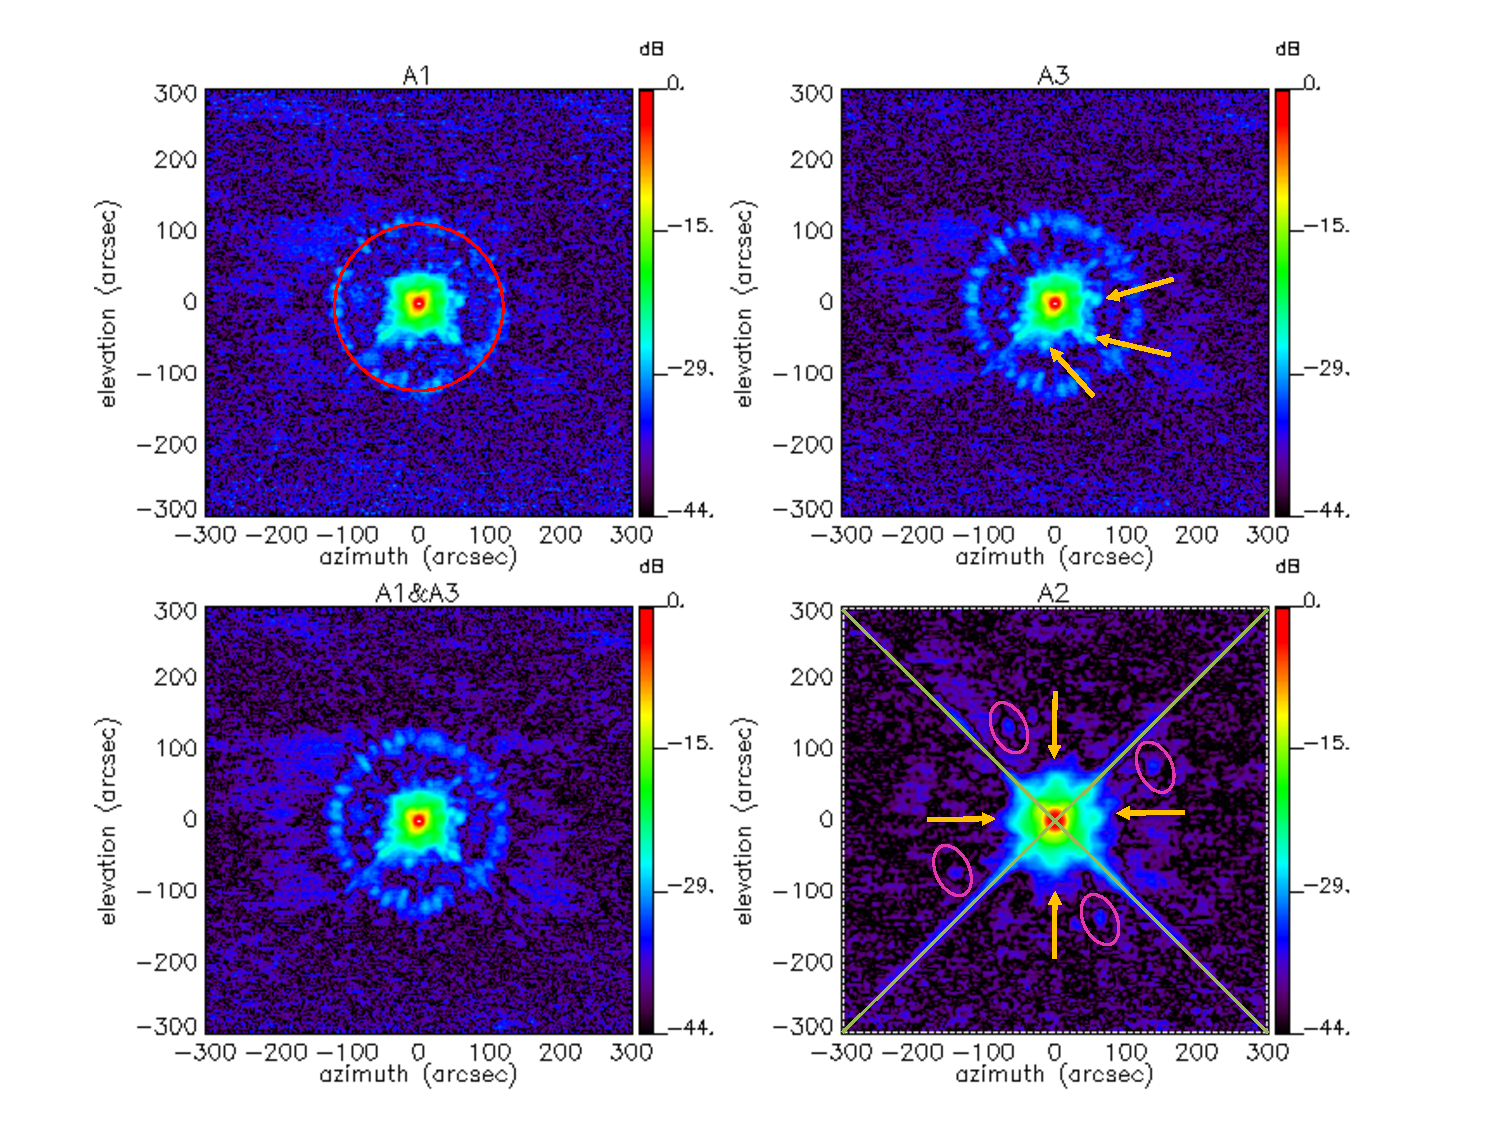
\includegraphics[clip, angle=0, scale=0.4]{Figures/Beams_features.pdf}
\caption{Noticeable features of NIKA2 beam pattern. Red circle: diffraction ring seen in 1-mm maps (the spokes are presumably caused by radial and azimuthal panel buckling (cf. Fig.4 in Greve et al. 2010)); Perpendicular green lines: diffraction pattern caused by quadrupod secondary support structure (prominently seen in 2mm maps); Yellow arrows in the upper right pannel: pattern of 3 spikes seen in 1mm maps of unknown origin; Yellow arrows in the lower right pannel: four symmetrical spokes of the first errorbeam; Pink ellipses: 4 spikes seen in 2mm maps.}
\label{fig:features}
\end{center}
\end{figure}

We further quantify the relative level of the main beam, the first error beam and other features seen in the 2D beam pattern using radial cuts.

[FIGURE JEAN-FRANCOIS]

\begin{figure}
\begin{center}
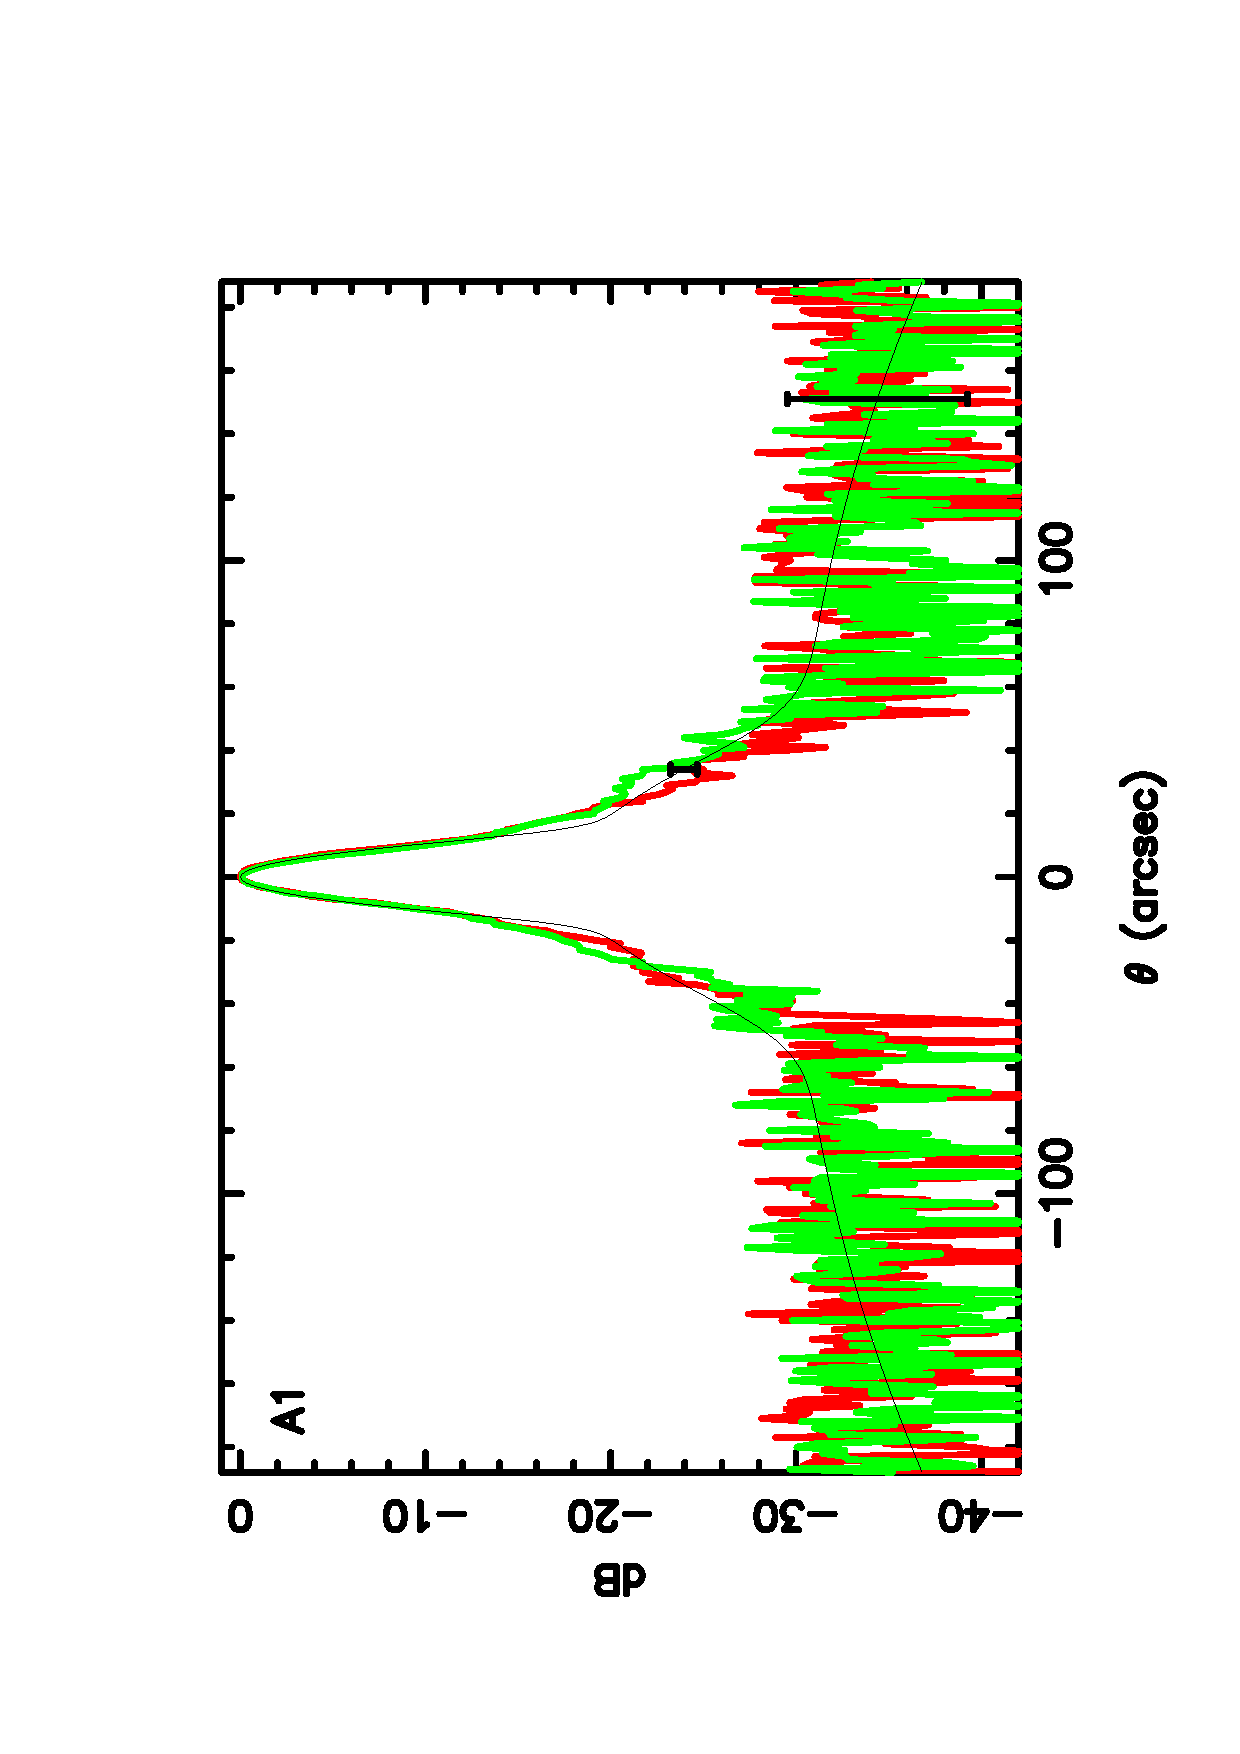
\includegraphics[clip, angle=-90, scale =0.3]{Figures/Array_A1_dB.pdf}
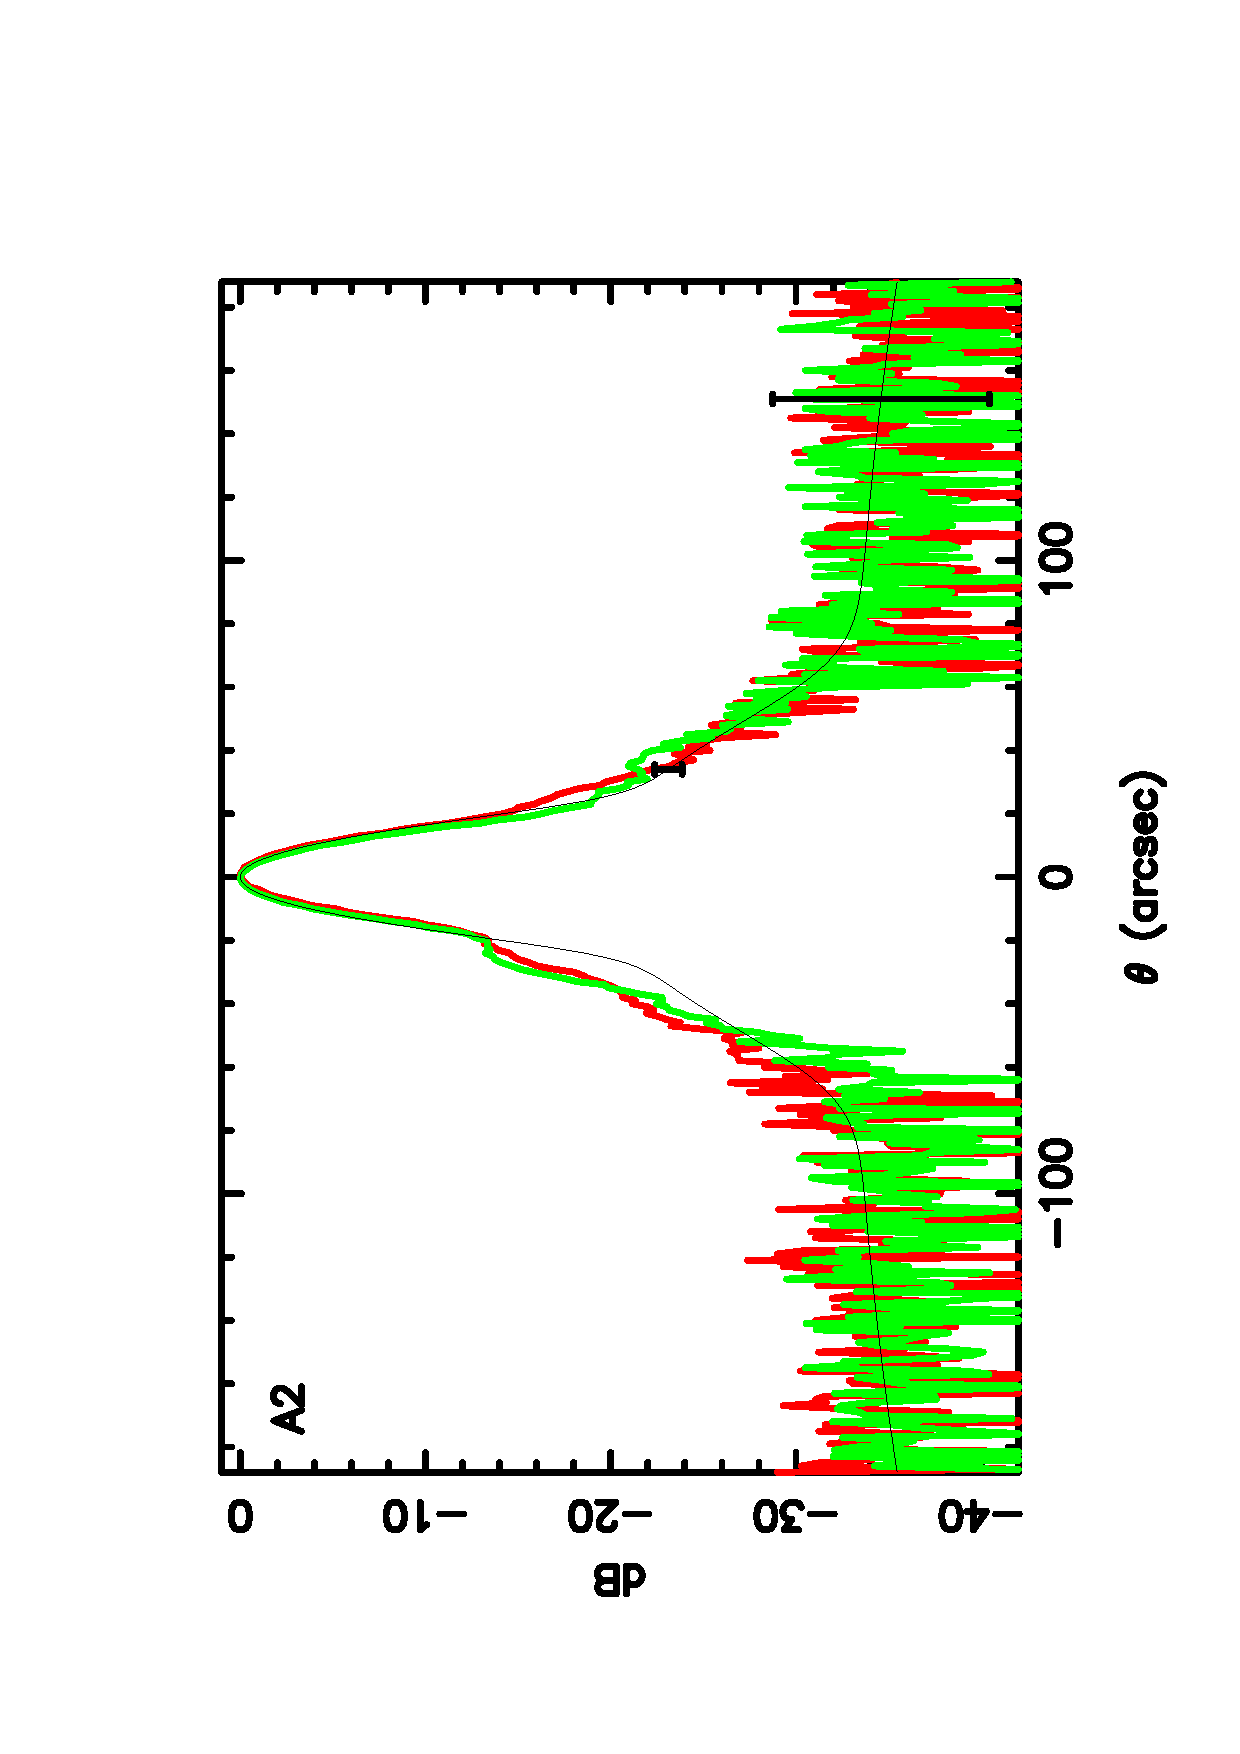
\includegraphics[clip, angle=-90, scale = 0.3]{Figures/Array_A2_dB.pdf}
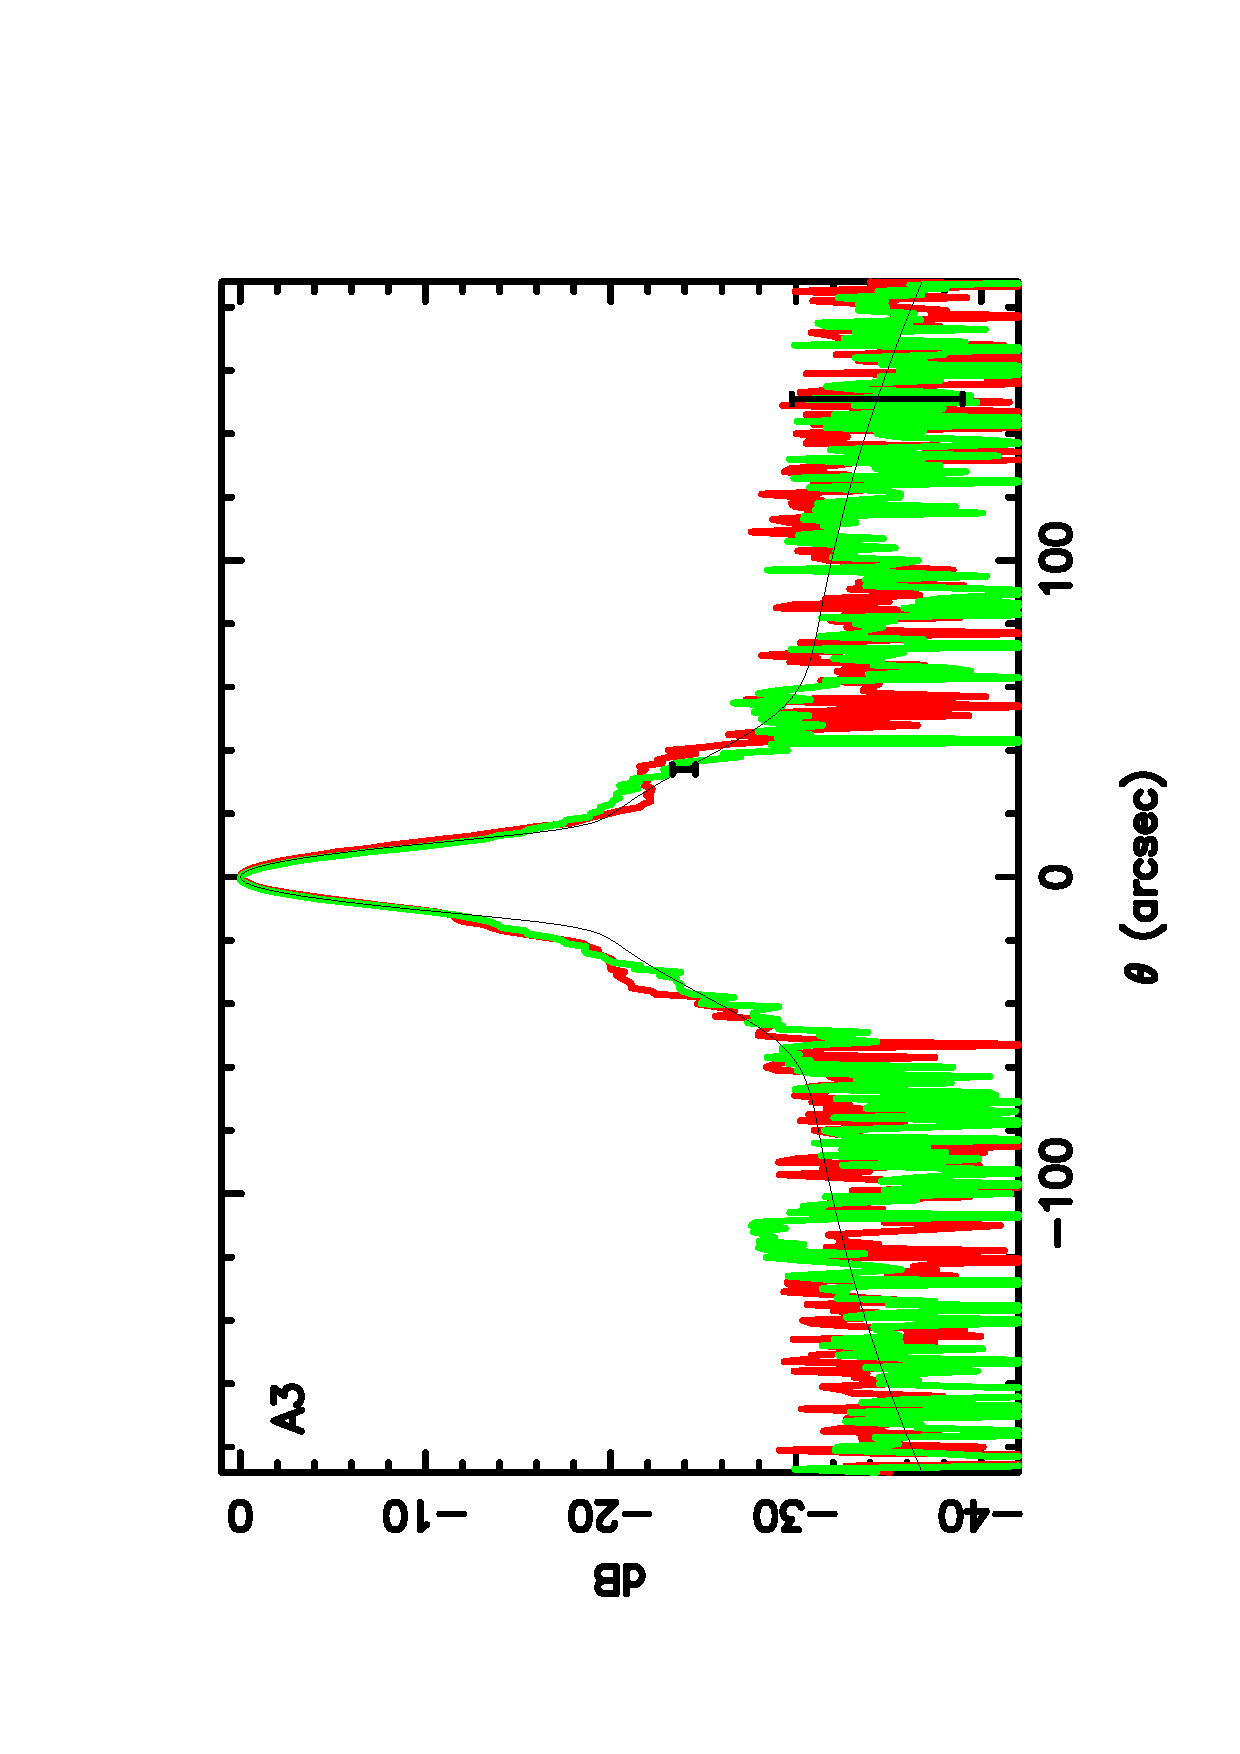
\includegraphics[clip, angle=-90, scale = 0.3]{Figures/Array_A3_dB.pdf}
\caption{Two orthogonal cuts through the beam are shown in red and green and a best fit model made
of three Gaussians is superimposed in black. These cuts were obtained from the high quality map of Uranus on 2017 January 25th.
The main beam starts to depart from the first Gaussian at -12dB. }
\label{fig:beam_dB3}
\end{center}
\end{figure}

The Iram 30-m beam as seen with NIKA2 is shown in
Fig. \ref{fig:beam_db} by means of two orthogonal cuts through Uranus
from a high quality map obtained on 2017 January 25th in excellent conditions
(low opacity $\tau_{225}=0.08$ and elevation $46^{\circ}$).
A model made of three Gaussians centered on the source peak was best
fit {\it by hand} to these cuts and the parameters are reported in
Table \ref{tab:3gauss} [PEUT-ETRE AVANTAGEUSEMENT REPLACED PAR VALEURS DE FLORIAN].
The main beam starts to depart from the first
Gaussian at the level of about -12dB for the three arrays.
We note that for the instrument EMIR on the radiotelescope,
this departure is about -20dB (Kramer, Penalver and Greve 2013).
From parameters in Table \ref{tab:3gauss}, one can estimate that
the source incident power is split about equally between the main beam
and the error beam at 1mm, and these fractions are 70\% and 30\% at 2mm, respectively.
This modelling uses the central
region   $180'' \times 180''$ in size with a uniform noise rms from
a larger area of 8' x 5' on the sky scanned with the arrays. It is expected
that the error beam extend beyond these limits.


\begin{table}
\centering 
\caption[]{Model parameters of the three Gaussian beam.}
\begin{tabular}{|l|l|l|l|l|l|l|}
\hline
               & \multicolumn{3}{c|}{A1 and A3} & \multicolumn{3}{c|}{A2}  \\
\hline
fwhm      & $11.25''$ & $45''$  & $250''$ & $17.75''$ & $56''$  & $420''$ \\
amplitude & 0.984     & 0.015   & 0.0005   &  0.9875   & 0.011   &  0.0005\\
\hline
\end{tabular}
\label{tab:3gauss}
\end{table}


\subsubsection{Beam profile}

\begin{figure*}[h!]
\centering
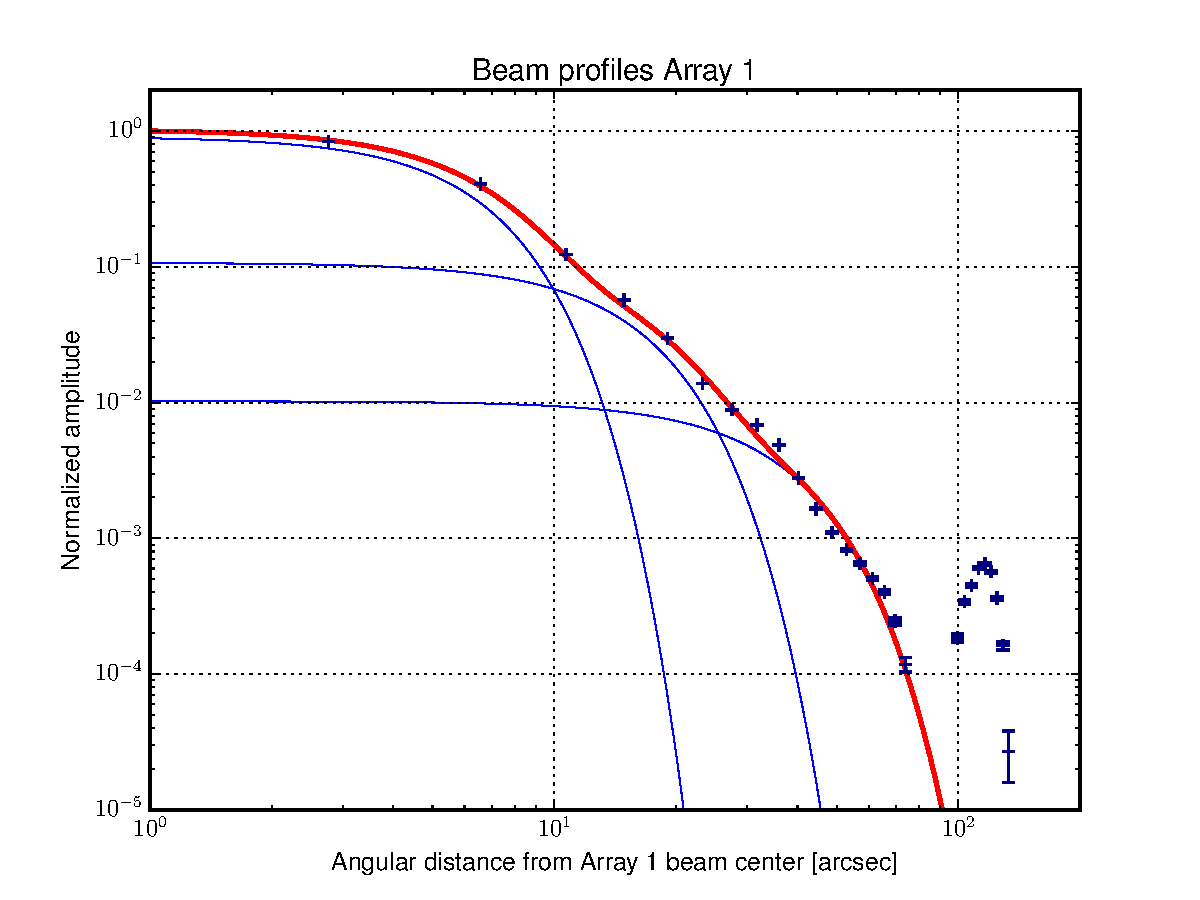
\includegraphics[height=6cm]{Figures/Beam_profiles_A1_FR.pdf}
\hspace{0.5cm}
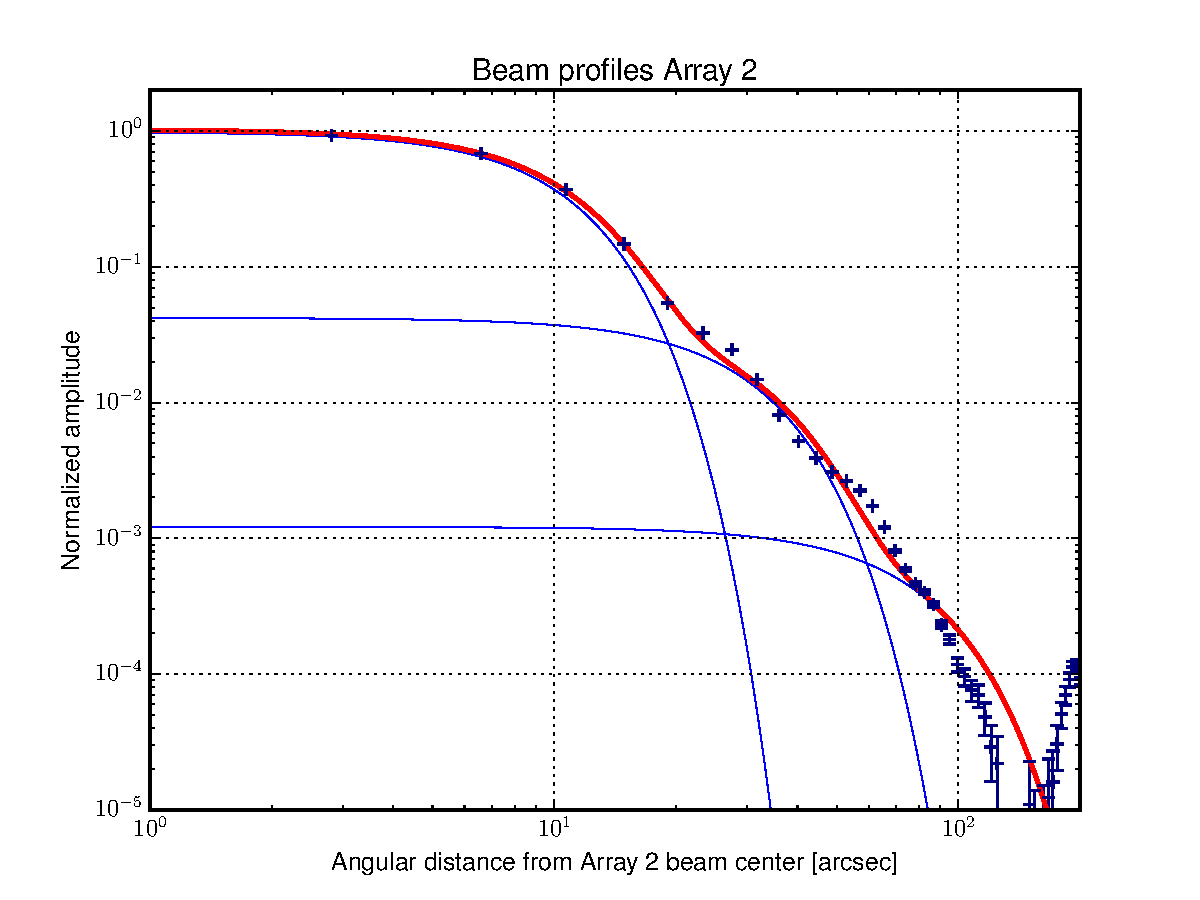
\includegraphics[height=6cm]{Figures/Beam_profiles_A2_FR.pdf}
\hspace{0.5cm}
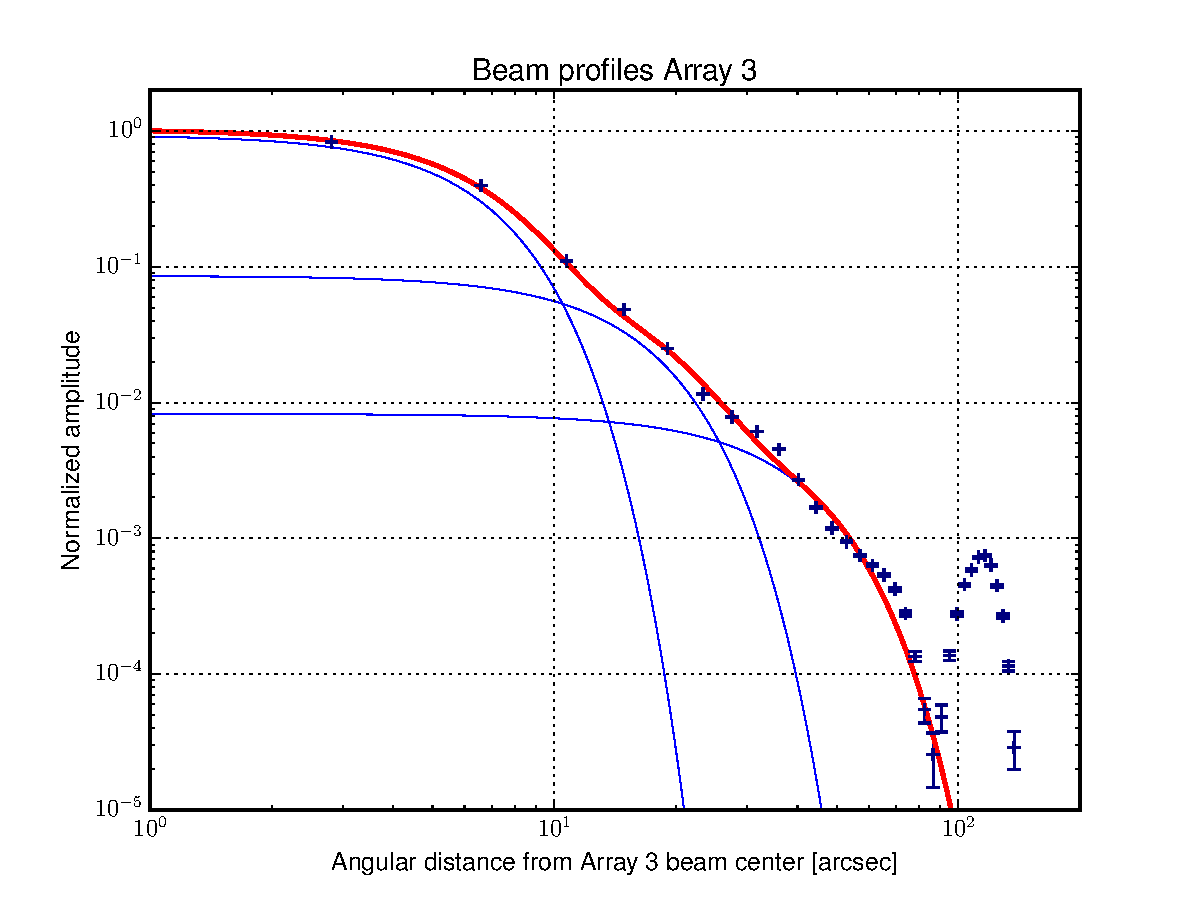
\includegraphics[height=6cm]{Figures/Beam_profiles_A3_FR.pdf}
\caption{{\footnotesize Beam profiles for array 1, 2, and 3.}}
\label{fig:beam_profiles_3G}
\end{figure*}


\subsubsection{Beam efficiency}


%% [STABILITY]
%%________________________________________________________
\subsection{Stability of the beam pattern}

[A FAIRE:

  AJOUTER LES PLOTS DE STABILITE EN FONCTION DE ELEVATION, TAU

]






%----------------------------------------------------------------------------------------
%	CALIBRATION
%----------------------------------------------------------------------------------------
\section{Calibration}
\label{se:calibration}

%
%%
%%
%%

%% [intro]

The calibration of the instrument NIKA2 in its final configuration
of January 24th 2017  is studied in this section  in using the 
 primary calibrators, Uranus and Neptune, and secondary calibrators ; the two largest asteroids Ceres and Vesta, and the three
planetary nebulae NGC7027, CRL2688, and MWC349.

\subsection{Reference flux densities of the calibrators}

The planets Uranus and Neptune are standard calibrators for many instruments,
{\it e.g.} PACS and SPIRES aboard Herschel and SCUBA2 at JCMT.
Their flux densities over a large spectrum from centimeter wavelengths to optical
are provided by the model of Moreno et al (1998) with an accuracy better than
5\% at millimeter wavelengths (Moreno, private communication). This model provides
flux densities for reference angular sizes $3.5''$
and $2.3''$ of Uranus and Neptune, respectively. They have been updated for run 9
with planetary distances at the reference date of 24th february 2017 with 
the JPL ephemerides \footnote{https://ssd.jpl.nasa.gov/horizons.cgi}.
They were computed at the central frequencies of the bandpasses of
the three arrays (255.21 GHz, 151.58 GHz, 257.92 GHz).

The asteroids Ceres and Vesta have been modeled by Muller et al (2014) in accounting for 
size, shape, spin-properties, albedo, and thermal properties and in adjusting to PACS, SPIRE and HIFI observations
of Herschel with an accuracy of 5\%. 
Thomas Mueller has tabulated flux densities at different wavelengths, in particular at 1300$\mu$m, every five days
until 2020 \footnote{http://www.iram.es/IRAMES/mainWiki/Continuum/Calibrators}.
We have used the prediction at  1300$\mu$m made for  23rd february 2017
and extrapolated it  to the central frequencies of the arrays in using a Rayleigh-Jeans
spectrum expected for Ceres and Vesta. Their flux densities in
Table~\ref{tab:fluxPred} are for this date. Over the five days of  run 9 (february 23 - 28), the
flux densities  at 1300$\mu$m  have decreased by  3\% 
for Ceres and  by 6\%  for Vesta in Muller's tables but we have not corrected for this effect in our analysis below.  

The secondary calibrator MWC349A is a young Be star, part of a stellar binary system, surrounded by a disk. Its radio
continuum emission originates in an ionized bipolar outflow (Tafoya et al 2004).
MWC349 has been monitored with the  Plateau de Bure interferometer
and shown to be only slightly angularly resolved, making it a point source for the 30-metre telescope. We have adopted
its flux densities from this monitoring \footnote{http://www.iram.fr/IRAMFR/IS/IS2012/presentations/krips-fluxcalibration.pdf}.
The secondary calibrator CRL2688 is an Asympotic Giant Branch star. Its radio continuum emission is mostly from circumstellar dust and
is somewhat extended  (Knapp et al 1994).
Its flux densities at $850\mu$m  and $450\mu$m  have been stable at the 5\% level as monitored by SCUBA2 (Dempsey et al 2013).
We have extrapolated their flux densities to the central frequencies
of the arrays with a power law of index $\alpha=-2.47$ derived from these SCUBA2 measurements.
The secondary calibrator NGC7027 is a young, dusty, carbon rich Planetary Nebula with an ionized core.
It is extended in the continuum and molecular lines (Bieging et al 1991) and  is not a point source for the telescope.
Its  most recent flux densities are reported at $1100\mu$m  and $2000\mu$m by Hoare et al (1992). It has been reported
to decrease by $\sim$ 0.145 percent/yr in the optically thin part of its spectrum above  $6$ GHz from VLA
observations (Zijlstra, van Hoof \& Perley 2008, and Hafez et al, 2008) that makes these flux densities uncertain by 3.6\%
at present. Its SED from cm wavelengths to optical is also presented in Hafez, Y.A. et al (2008).
The flux densities adopted at the central frequencies of the arrays for these three calibrators are in Table~\ref{tab:fluxPred}.


\begin{table}
\centering
\label{tab:fluxPred}
\caption[]{Reference flux densities of calibrators at central frequencies of arrays.}
\begin{tabular}{|l|c|c|c|}
\hline
\multicolumn{1}{|c}{}  & \multicolumn{3}{|c|}{flux densities (Jy)}  \\
\hline
         &    A1      &  A2   &   A3    \\
         &  255GHz    & 152GHz  &  258GHz \\
\hline
Uranus   &  37.12   & 16.35 &  37.810 \\
Neptune  &  15.28   &  6.84 &  15.58  \\
Vesta    &   0.99   &  0.35 &   1.01  \\
Ceres    &   0.89   &  0.31 &   0.91   \\
MWC349   &   2.2    &  1.6  &   2.2   \\
NGC7027  &   3.61   &  4.42 &   3.61  \\
CRL2688  &   3.03   &  0.83 &   3.03  \\
\hline
\end{tabular}
%\label{tab:fluxPred}
\end{table}


\subsection{Aperture photometry}

The calibrators were observed frequently during run9. These observations were beammaps for Uranus and Neptune
as well as  sequences of 4 consecutive
otf maps ($8' \times 5'$) as done for Ceres Vesta, NGC7027, CRL2688, and MWC349. All observations were processed 
to produce intensity maps for the three arrays with the pipeline  in
using kidpar
{\it kidpar-best3files-FXDC0C1-GaussPhot} for the array geometry,
the method {\it COMMON-MODE-ONE-BLOCK}  to remove
 low frequency noise including atmosphere,
sky projection AZEL, line-of-sight opacities, an {\it a priori} mask of $100''$ and no iteration in mapping.
Note that the gain variation with elevation from EMIR implemented in the pipeline has not been used. 
In addition to the fact that they  have flux densities accurately known from models,
Uranus and Neptune are significantly stronger than the other calibrators, and  are the best sources to caracterize the
instrument and calibrate its flux density  scale.

The total flux densities of all twenty eight observations of Uranus and Neptune during run 9 were
measured directly with aperture photometry over a large radius of 150'' to reach saturation level in including the most significant part of the
error beam of the telescope. These flux densities from all twenty eight individual observations are in Table~\ref{tab:fluxAp} ; each observation
is either a 4 minute long  otf $8' \times 5'$ in size (o) or  a 20 minute long beammap (b). These measurements are of high quality
over a broad range of observing conditions
($33^{\circ}<$ elevations $<58^{\circ}$, and   $0.16 < \tau_{1mm} < 0.50$, see details in  Table~\ref{tab:fluxAp}). An illustration of
our aperture photometry is given in Fig.~\ref{fig:PhAp}.

We emphasize that prior to summation of all the pixels within the aperture, the intensity of each pixel must be estimated
from its brightness  given in Jy/beam in the map provided by the
pipeline. Here, beam stands  for the whole beam which is commonly 
described by the main beam and side lobes, or error beam. The brightness of each pixel must be multiplied by
$dx \times dx / \Omega_{true}$ where  $dx$ is the pixel size ($1''$ in our processing)
and $\Omega_{true}$  is the solid angle of the true beam.
We have computed the solid angle of the true beam as
$ \Omega_{true} (r_{max}) = \int_0^{2\pi} \int_0^{r_{max}} B(r) 2 \pi r dr$, where
$B(r)$ is the radial profile of the azimuthally averaged brigthness over narrow annuli,  $dr$ in width, and normalised so that B(0)=1.
We have used conservatively $r_{max}=250''$ since $ \Omega_{true}$  saturates at $r_{max}=150''$ as does photometry as illustrated
in Fig.~\ref{fig:PhAp}. This integral is derived from the general expression ({\it e.g.} Adam, 2016, \S 8.1.1.2 of his PhD thesis) for a
brightness distribution assumed azimuthally symmetric.  The excess
of the true beam relative to the Gaussian beam is $\Omega_{true} / 2 \pi (\sigma_{Gauss})^2$, with  $\sigma_{Gauss}$ derived from
the $FWHM$ of each observation. These excesses have been 
estimated  for all 28 observations of Uranus and Neptune in run 9 and are shown in Fig.~\ref{hist:excesses}.

%Their means and rms :  
%???  $1.72 \pm 0.12 $, $ 1.33 \pm 0.04$, and $1.68\pm 0.13$  SHOULD BE 1.5 - 1.6 at 1mm ???   for arrays A1, A2 and A3, respectively. 
%These excesses were 1.34 and 1.28 at 1mm and 2mm, respectively, for NIKA (Adam 2016).
%These excesses reflect the fraction of the
%source power that goes into the side lobes of the telescope.

The determination of $FWHM$ and $\Omega_{true}$  for each observation
makes the resulting photometry relative.


\subsection{Relative photometry of Uranus and Neptune}

To caracterize our relative photometry of Uranus and Neptune, we show in Fig.~\ref{fig:U_N_ratio} the ratio between these measured flux densities
and their reference values given in Table~\label{tab:fluxPred}.
For all twenty eight individual observations of run 9, the resulting means are 1.005,  1.019, and 1.027
for array 1, array 2, and array 3, respectively. This is a systematic bias of less than 3\% with respect to the model values.
The resulting rms are 4.0\%, 2.6\%, and 3.8\%, relative to these means, and indicate
a scatter at the 4\% level in our relative photometry.  These results are consistent with the uncertainty of less than
$5\%$ claimed for the models of Moreno et al for Uranus and Neptune.

In Fig.~\ref{fig:U_N_ratio}, these flux density ratios are plotted versus elevation and airmass but no apparent correlation is found.
We recall that the gain curve of EMIR implemented in the pipeline was not used for the processing. It might be
that the lack of correlation with elevation is due to
the limited range of elevations  between 33$^{\circ}$ and 58$^{\circ}$ covered by these observations.

Finally, in Fig.~\ref{fig:U_N_corr},  we find that the flux density
variations are correlated between the three arrays.

\begin{table}
%\centering
\label{tab:fluxAp}
\caption[]{Measured flux densities of primary calibrators.}
\begin{tabular}{|l|l|r|c|c|c|c|c|c|}
\hline
\multicolumn{1}{|c}{} & \multicolumn{1}{|c}{observation} & \multicolumn{1}{|c}{}  & \multicolumn{1}{|c}{elev. } &  \multicolumn{1}{|c}{$\tau_{1mm} $}  &  \multicolumn{1}{|c}{$\tau_{2mm} $ } & \multicolumn{3}{|c|}{flux densities (Jy)}  \\
\hline
          &              &         &  ($^{\circ}$)   &      &      &              A1              &                         A2   &                       A3    \\
\hline
 Uranus   & 20170223s46  & b  & 37.9 & 0.48 & 0.31 & $     35.74 \pm        1.18$  & $     16.78 \pm        0.27$ & $     37.80 \pm       0.97$  \\
 Neptune  & 20170224s177 & b   & 39.2 & 0.50 & 0.34 & $     16.05 \pm        0.93$  & $      7.41 \pm        0.17$ & $     17.20 \pm       0.78$  \\
 Uranus   & 20170225s222 & b   & 35.9 & 0.28 & 0.18 & $     38.34 \pm        0.74$  & $     16.69 \pm        0.23$ & $     39.02 \pm       0.63$  \\
 Uranus   & 20170225s266 & o   & 57.1 & 0.28 & 0.18 & $     36.44 \pm        1.17$  & $     16.08 \pm        0.34$ & $     37.57 \pm       0.96$  \\
 Uranus   & 20170225s267 & o &  57.5 & 0.28 & 0.19 & $     40.98 \pm        1.23$  & $     16.94 \pm        0.34$ & $     42.14 \pm       1.04$  \\
 Uranus   & 20170225s268 & o &  57.9 & 0.28 & 0.18 & $     38.47 \pm        1.20$  & $     17.16 \pm        0.45$ & $     39.85 \pm       1.03$  \\
 Uranus   & 20170225s269 & o &  58.2 & 0.28 & 0.19 & $     37.54 \pm        1.22$  & $     16.83 \pm        0.39$ & $     41.45 \pm       1.10$  \\
 Uranus   & 20170227s304 & o &  58.8 & 0.14 & 0.12 & $     38.33 \pm        0.93$  & $     16.66 \pm        0.33$ & $     39.85 \pm       0.82$  \\
 Uranus   & 20170227s305 & o &  58.5 & 0.15 & 0.12 & $     36.23 \pm        0.89$  & $     15.97 \pm        0.32$ & $     38.48 \pm       0.78$  \\
 Uranus   & 20170227s306 & o &  58.1 & 0.16 & 0.13 & $     35.69 \pm        0.92$  & $     15.89 \pm        0.38$ & $     36.63 \pm       0.79$  \\
 Uranus   & 20170227s307 & o & 57.7 & 0.16 & 0.13 & $     36.64 \pm        0.96$  & $     16.13 \pm        0.35$ & $     36.56 \pm       0.86$  \\
 Uranus   & 20170227s308 & b & 56.1 & 0.17 & 0.14 & $     36.88 \pm        0.61$  & $     16.35 \pm        0.24$ & $     38.55 \pm       0.52$  \\
 Uranus   & 20170227s315 & o & 53.0 & 0.18 & 0.14 & $     39.36 \pm        0.99$  & $     16.89 \pm        0.32$ & $     39.47 \pm       0.88$  \\
 Uranus   & 20170227s316 & o & 52.4 & 0.19 & 0.14 & $     37.25 \pm        1.03$  & $     16.82 \pm        0.32$ & $     39.87 \pm       0.90$  \\
 Uranus   & 20170227s317 & o & 51.9 & 0.19 & 0.14 & $     39.47 \pm        1.14$  & $     16.70 \pm        0.34$ & $     40.03 \pm       0.99$  \\
 Uranus   & 20170227s318 & o & 51.3 & 0.19 & 0.15 & $     36.49 \pm        1.06$  & $     16.58 \pm        0.32$ & $     39.27 \pm       0.92$  \\
 Uranus   & 20170227s321 & o & 48.5 & 0.19 & 0.15 & $     36.05 \pm        1.09$  & $     16.64 \pm        0.35$ & $     38.75 \pm       1.00$  \\
 Uranus   & 20170227s322 & o & 47.9 & 0.20 & 0.15 & $     35.11 \pm        1.04$  & $     16.30 \pm        0.33$ & $     37.42 \pm       0.93$  \\
 Uranus   & 20170227s323 & o & 47.2 & 0.19 & 0.14 & $     35.90 \pm        1.08$  & $     16.02 \pm        0.34$ & $     37.93 \pm       1.02$  \\
 Uranus   & 20170227s324 & o & 46.6 & 0.18 & 0.14 & $     35.05 \pm        1.04$  & $     16.05 \pm        0.32$ & $     36.96 \pm       0.93$  \\
 Uranus   & 20170227s352 & o & 39.0 & 0.24 & 0.18 & $     38.91 \pm        1.35$  & $     17.18 \pm        0.37$ & $     40.20 \pm       1.12$  \\
 Uranus   & 20170227s353 & o & 38.3 & 0.24 & 0.18 & $     38.21 \pm        1.27$  & $     16.99 \pm        0.38$ & $     39.32 \pm       1.06$  \\
 Uranus   & 20170227s354 & o & 37.6 & 0.23 & 0.17 & $     38.90 \pm        1.35$  & $     17.25 \pm        0.41$ & $     39.45 \pm       1.10$  \\
 Uranus   & 20170227s355 & o & 36.9 & 0.23 & 0.17 & $     38.49 \pm        1.36$  & $     16.66 \pm        0.33$ & $     38.80 \pm       1.11$  \\
 Uranus   & 20170227s356 & o & 36.1 & 0.23 & 0.17 & $     36.09 \pm        1.35$  & $     17.13 \pm        0.36$ & $     37.73 \pm       1.14$  \\
 Uranus   & 20170227s357 & o & 35.4 & 0.23 & 0.17 & $     37.17 \pm        1.36$  & $     16.66 \pm        0.38$ & $     37.29 \pm       1.13$  \\
 Uranus   & 20170227s358 & o & 34.6 & 0.23 & 0.17 & $     36.70 \pm        1.30$  & $     16.69 \pm        0.41$ & $     38.33 \pm       1.15$  \\
 Uranus   & 20170227s359 & o & 33.9 & 0.22 & 0.17 & $     35.43 \pm        1.21$  & $     16.60 \pm        0.42$ & $     36.60 \pm       1.04$  \\
\hline
\end{tabular}
%\begin{tablenotes}
b : beammap \filbreak
o : 4 $\times$ otf
%\end{tablenotes}
%\label{tab:fluxAp}
\end{table}

\begin{figure}
\begin{center}
  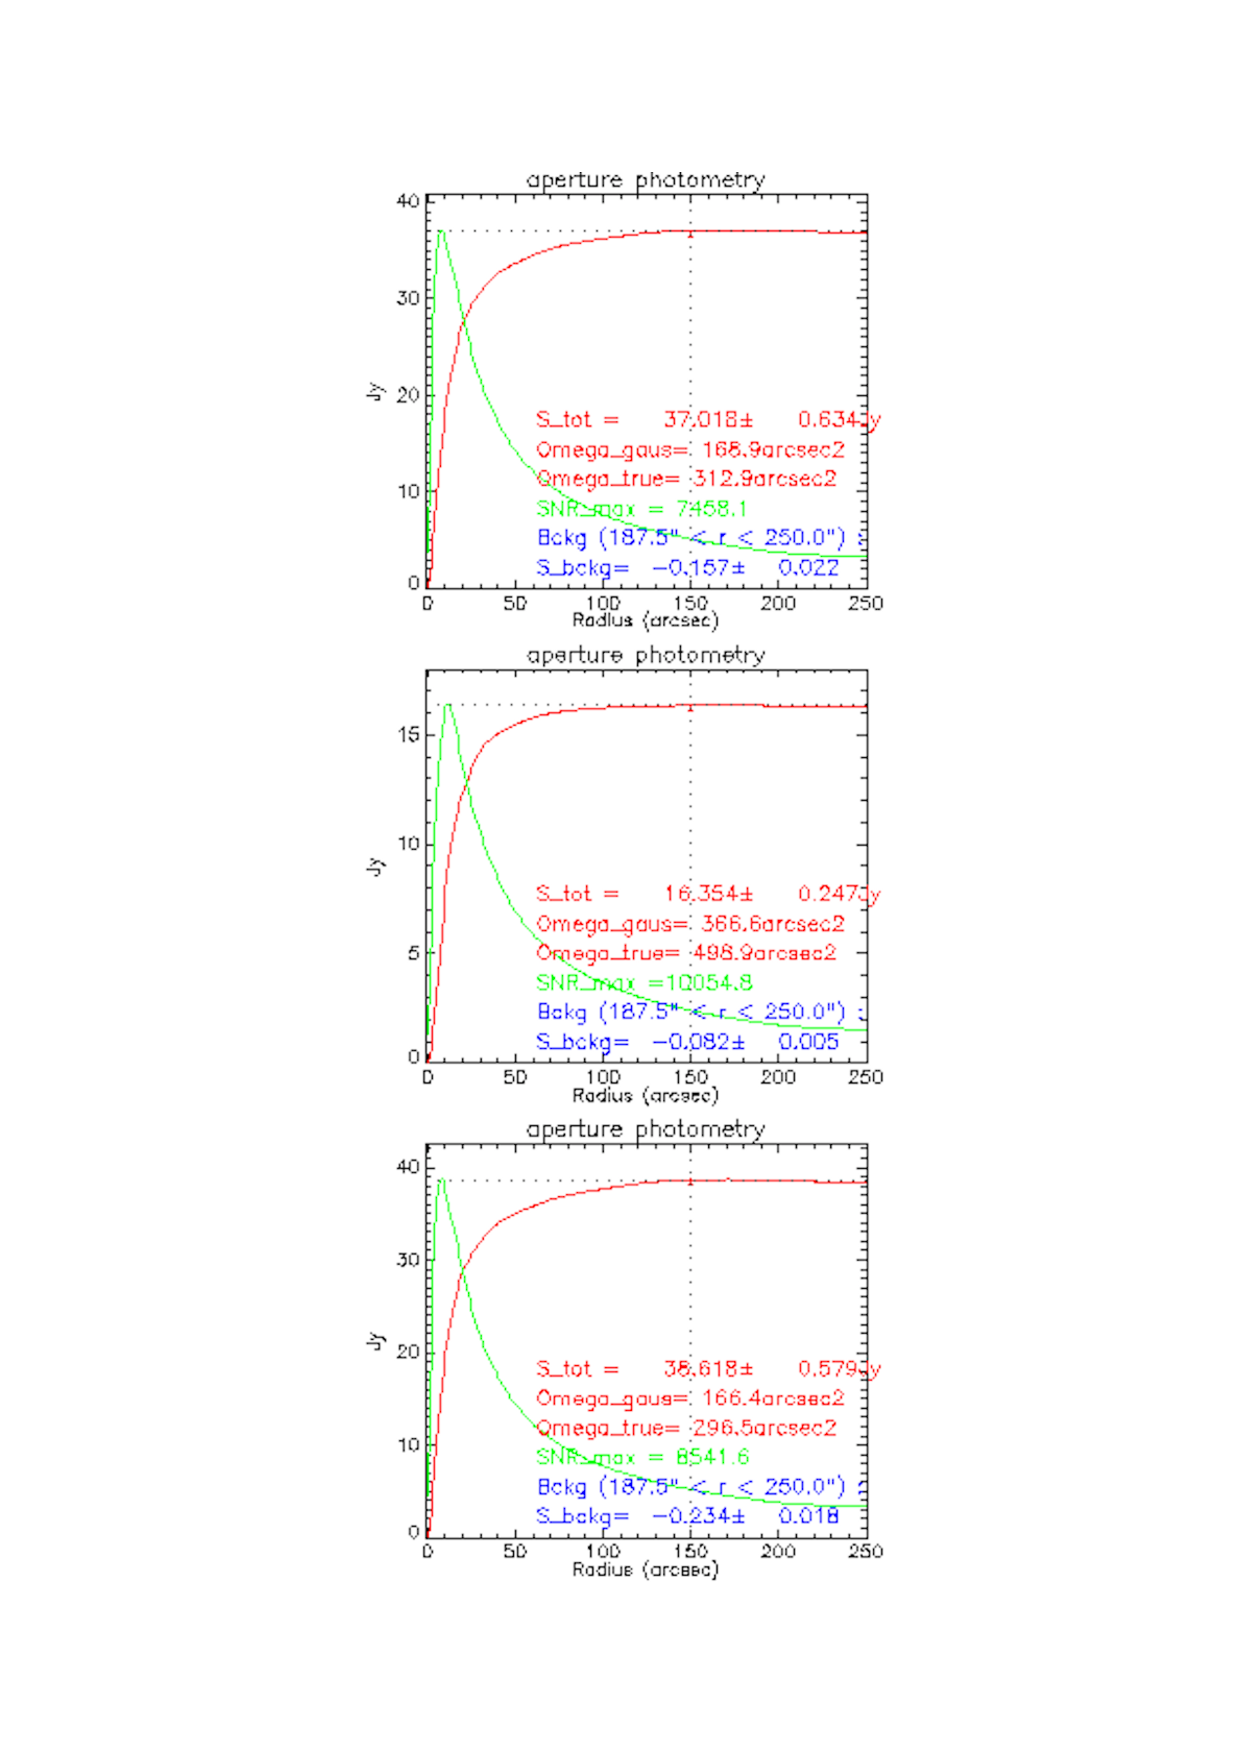
\includegraphics[clip, angle=0, scale=0.4]{Figures/Uranus_s308.pdf}
  \caption{Aperture photometry of Uranus observation 20170227s308  on array 1, 2 and 3 from top to bottom.
    The photometric curve in red saturates at about the radial distance of $150''$ from the
    source brightness center with a precision of a small fraction of Jy. (Green curve is the SNR in individual annulus but can be ignored for this
  presentation; GREEN CURVE WILL BE DELETED FOR VERSION DRAFT, IF FIGURE STAYS)}
\label{fig:PhAp}
\end{center}
\end{figure}

\begin{figure}
\begin{center}
  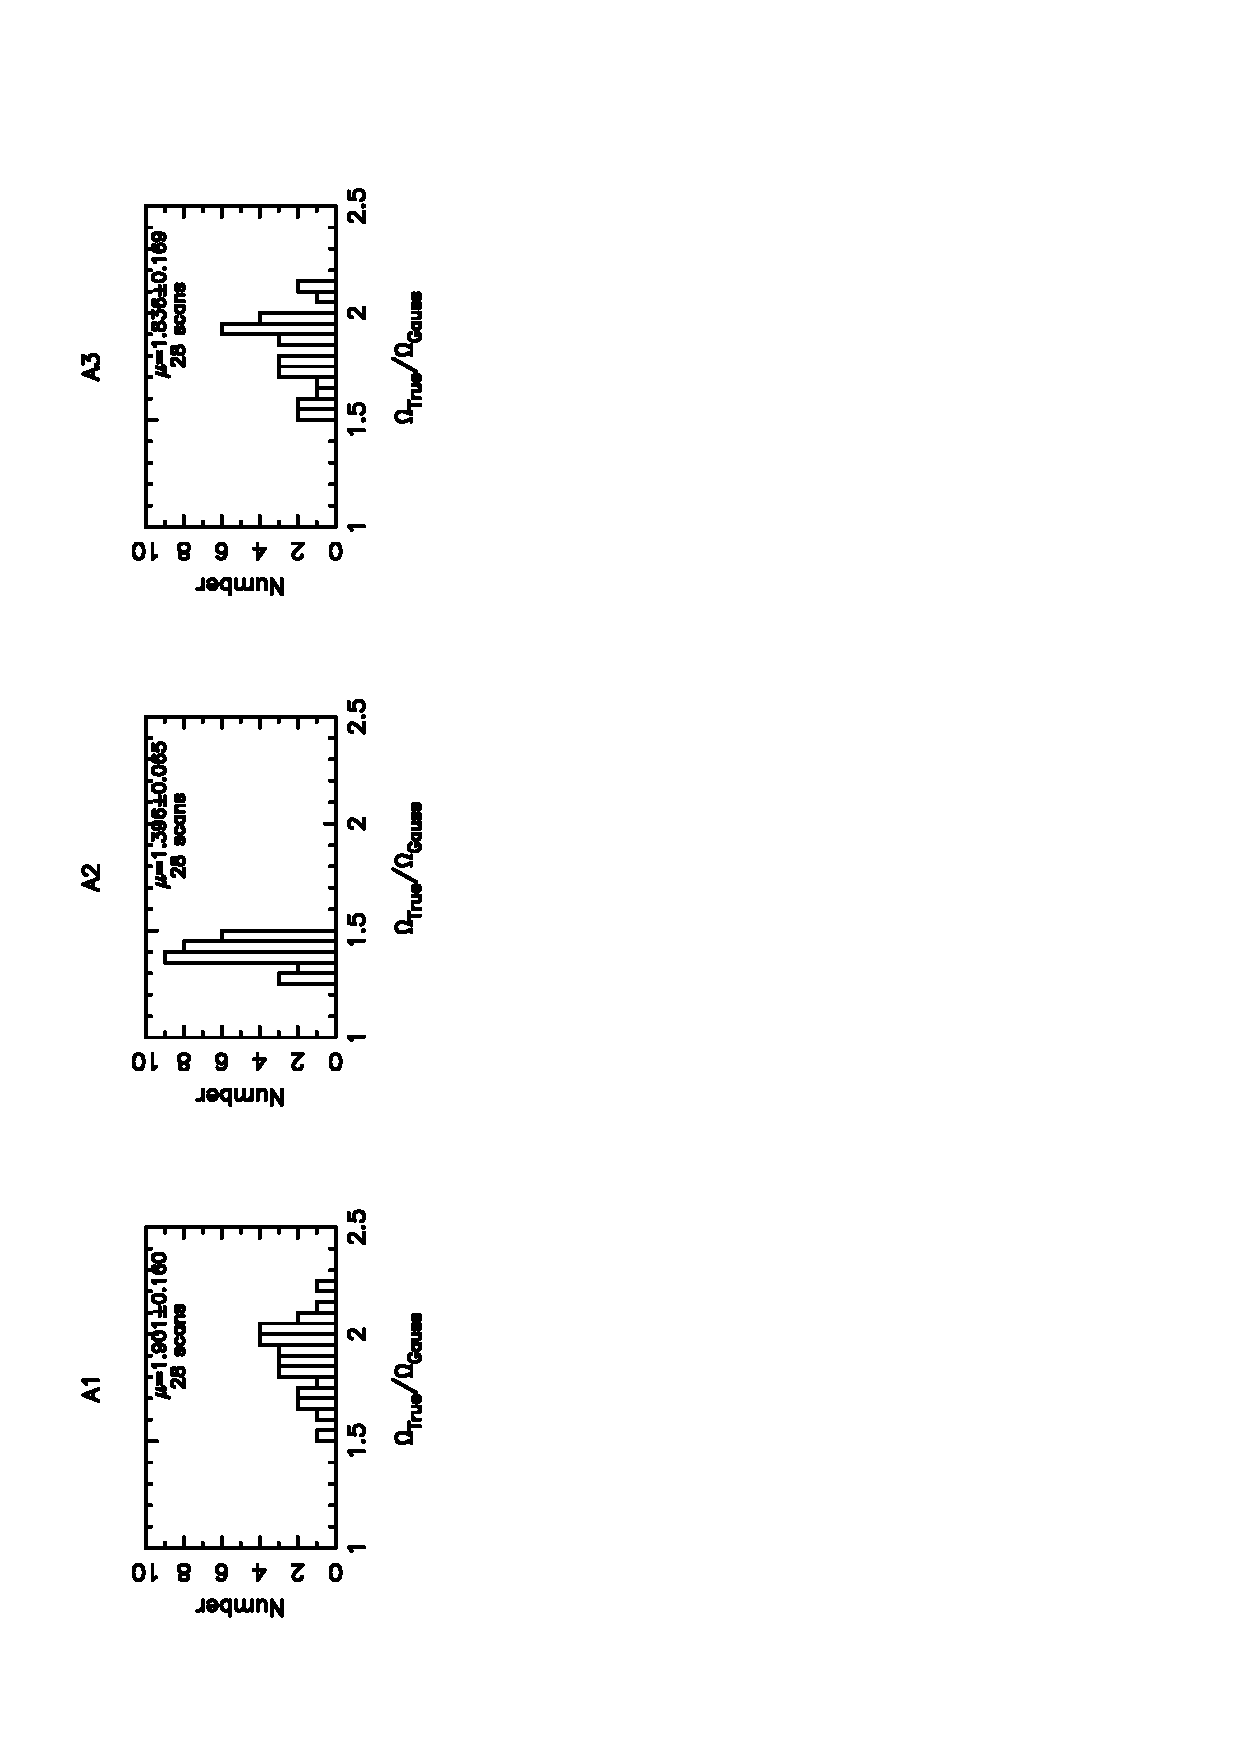
\includegraphics[clip, angle=-90, scale=0.6]{Figures/TG_hist_Ura_Nep_run9_28scan.pdf}
  \caption{Histogram of the excesses in solid angle between the true beam and the Gaussian beam for all
   observations of Uranus and Neptune during run 9.}
\label{hist:excesses}
\end{center}
\end{figure}

\begin{figure}
\begin{center}
  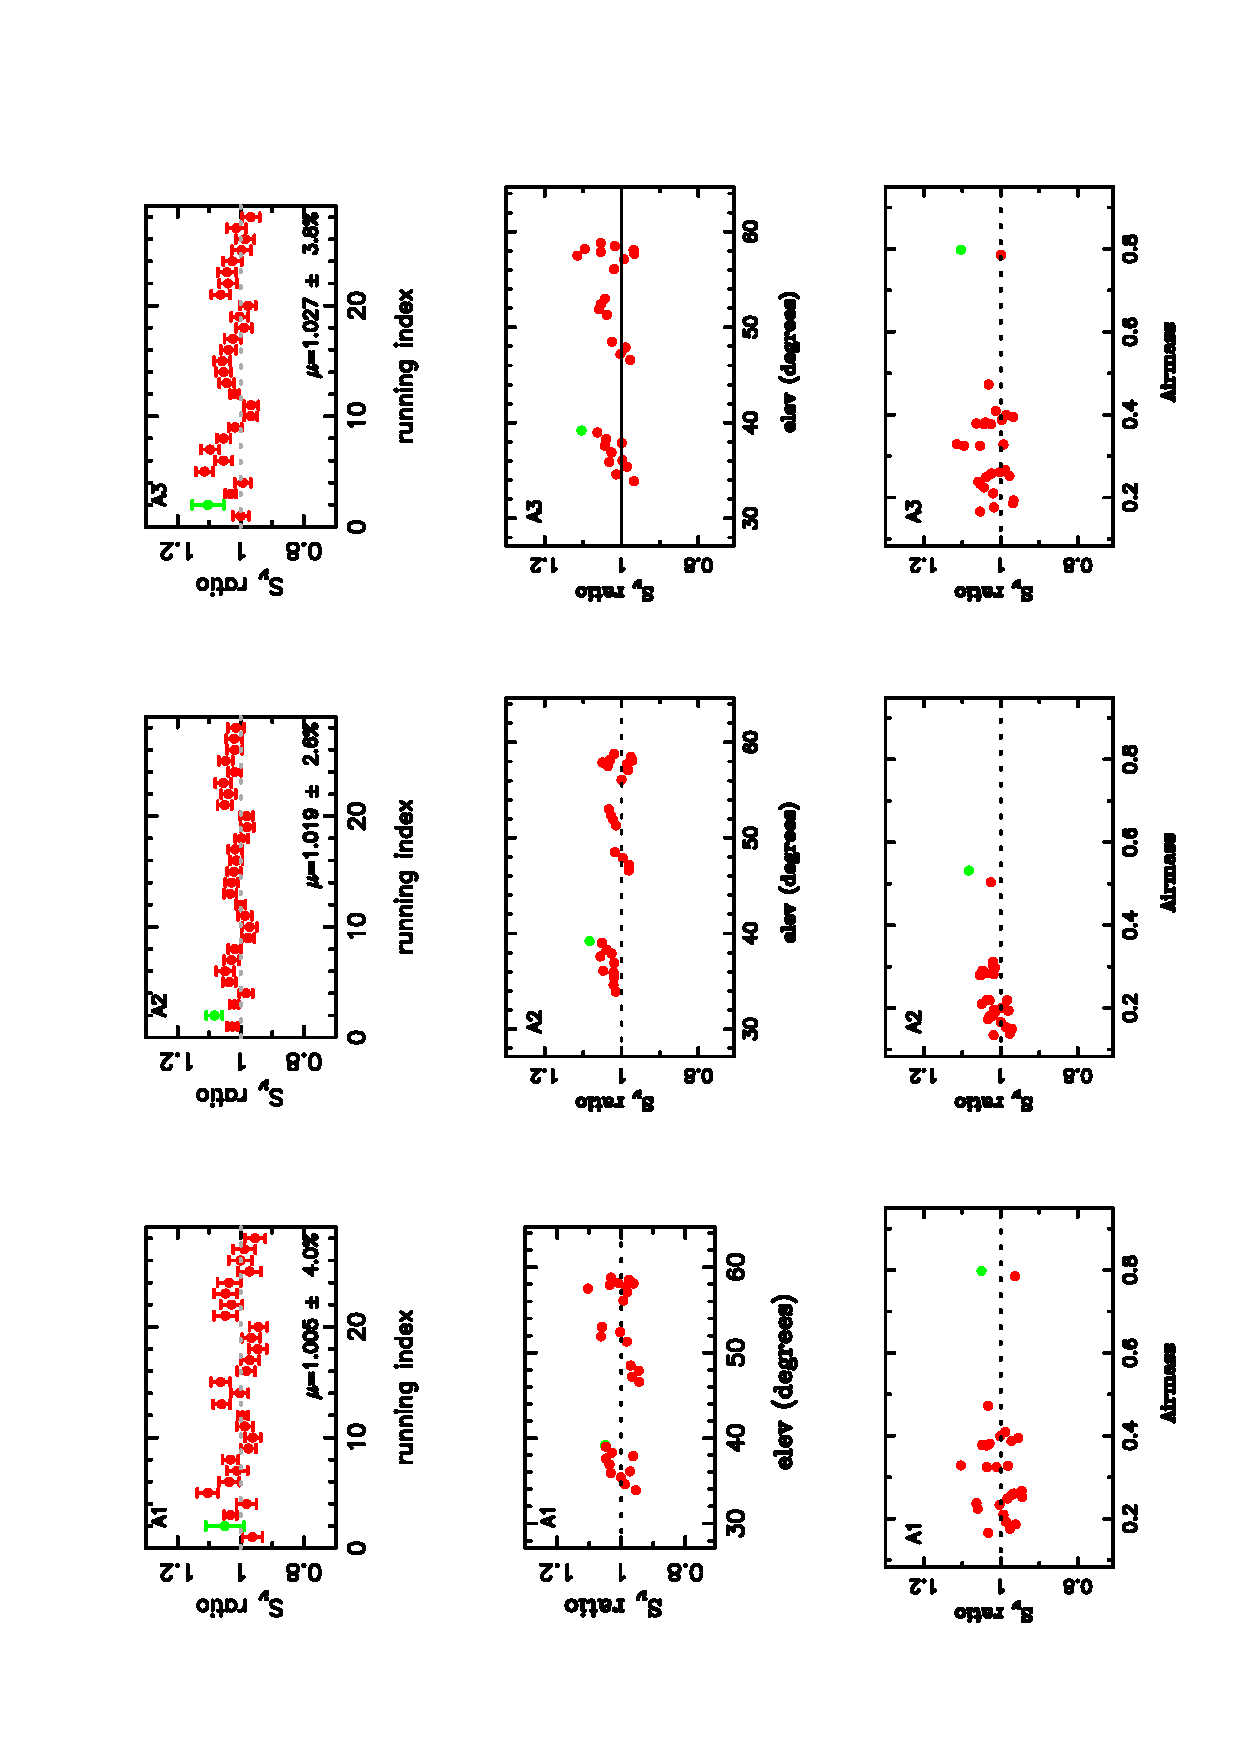
\includegraphics[clip, angle=-90, scale=0.6]{Figures/Ura_Nep_ratio_index_elev_airmass.pdf}
  \caption{Ratios between measured and reference flux densities for all observations of Uranus and Neptune during run 9.
    Red is for Uranus and Green is for Neptune.  (DATA FILE : cal-single-obs-AZEL.dat)}
\label{fig:U_N_ratio}
\end{center}
\end{figure}

\begin{figure}
%\begin{center}                                                                                                                                               
  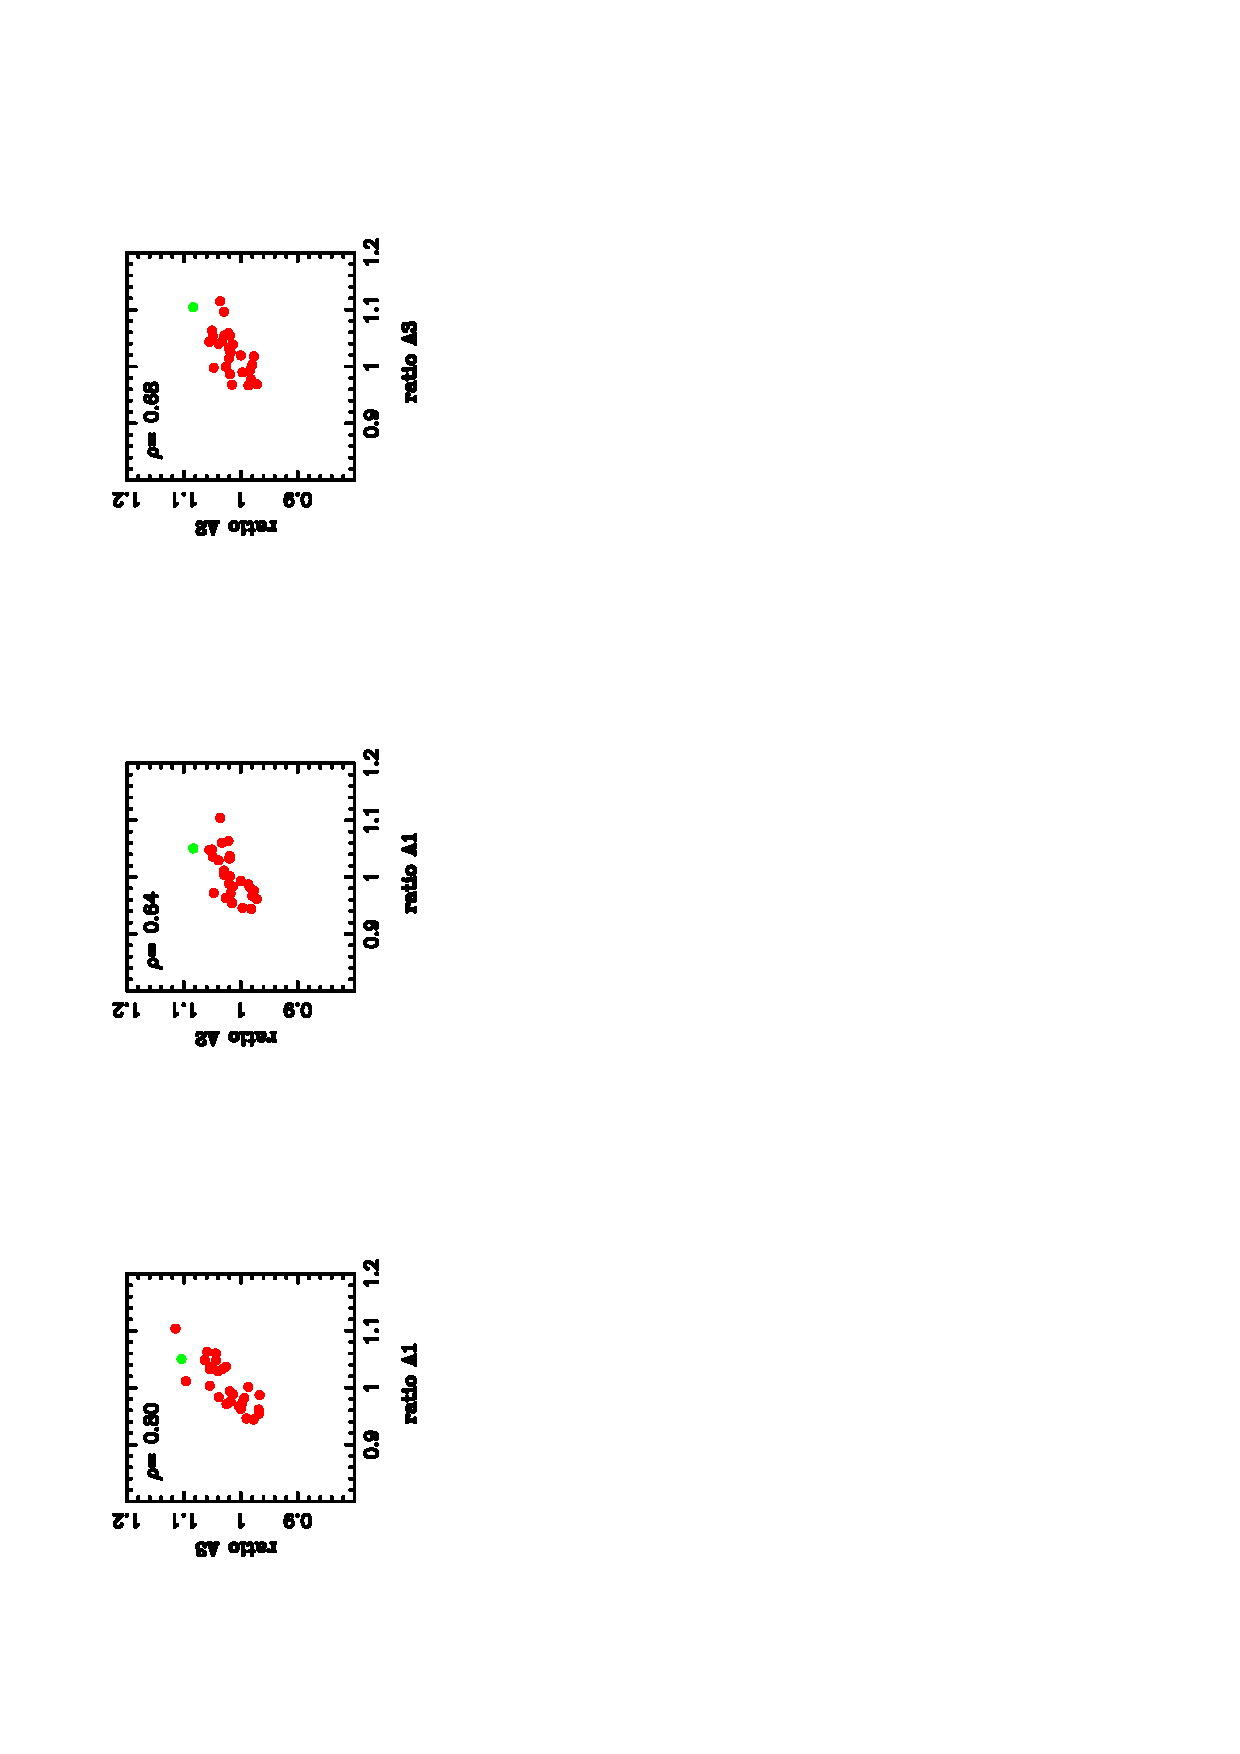
\includegraphics[clip, angle=-90, scale=0.65]{Figures/Ura_Nept_correlation_plots.pdf}
  \caption{Correlation plots between  the three arrays for all
    observations of Uranus and Neptune during run 9. Correlation
    coefficients $\rho$ are given.}
\label{fig:U_N_corr}
%\end{center}                                                                                                                                                 
\end{figure}



%We have extended this  analysis to all the secondary calibrators (Ceres, Vesta, NGC7027, MWC349, CRL2688)
%observed during run 9. As for the planets, the observations were processed with the pipeline including line-of-sight opacity.
%Aperture photometry was carried out and the solid angle $\Omega_{true}$  estimated from each map,
%except for Ceres and Vesta which are too faint. Four observations of secondary calibrators were discarded because
%aperture photometry failed to converge. The fifty three observations remaining provided flux densities on the three
%arrays that were compared to their reference flux densities given in Table~\ref{tab:fluxPred}. Their  ratios
% were plotted in Fig.~\ref{fig:all} in time order.
%The eleven flux density  measurements of CRL2688 were all clearly too high  and were multiplied
%by the factors 0.9 at 1mm and 0.75 at 2mm to yield the ratios shown in Fig.~\ref{fig:all}. Also, the flux density of Ceres at 1mm
%in Table~\ref{tab:fluxPred} is too low  but we did not correct for it because the flux densities of the four observations
%of Ceres have large uncertainties. This is apparent in the plot. The first obsertions of the strong source
%Uranus (index 1 in plot) and Neptune (index 11 in plot) in mediocre weather during the first half of the run
%do not show any degradation in the plot while secondary calibrators do. Overall,  the observations of
%all calibrators, primary and secondary, with minimal selection (four discarded out of fifty seven) and 
%a simple adjustement for calibrator CR2688, yield an absolute calibration stable  at the level
%of 14\% for array A1, 8.1\% for array A2, and 16.7\% for array A3, during run 9
%in  Fig.~\ref{fig:all}. In addition, no correlation is apparent with opacities, elevation, or airmass
%as shown in  Fig.~\ref{fig:versus_all}.

























\begin{figure}
\begin{center}
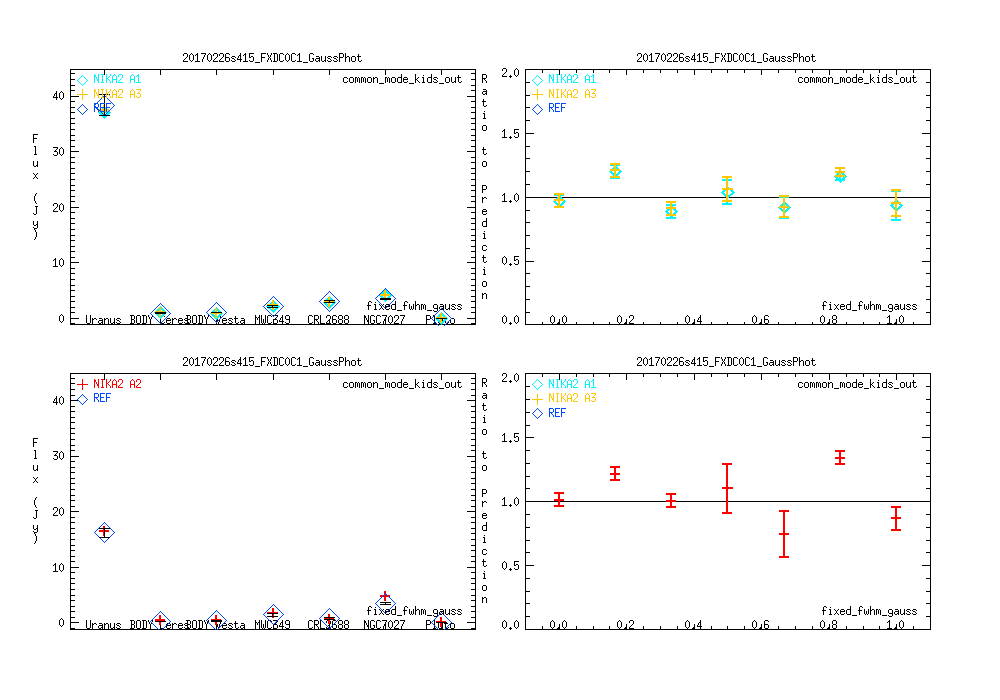
\includegraphics[clip, angle=0, scale = 0.4]{Figures/Calibrators_N2R9_20170226s415_FXDC0C1_GaussPhotFluxType_fixed_fwhm_gauss.png}
\caption{Decorrelation mask: 100 or 60 arcsec, KID cross-calib with fixed fwhm
  (12.5 and 18.5), then absolute photometry with the same fixed fwhm. Note:
  NGC7027 not point like and not corrected for here. Error bars from NIKA2
  measurements and abs. cal. uncertainties by JFL.}
\label{fig:fov}
\end{center}
\end{figure}


\subsection{Calibration stability across the run}

\begin{figure}
\begin{center}
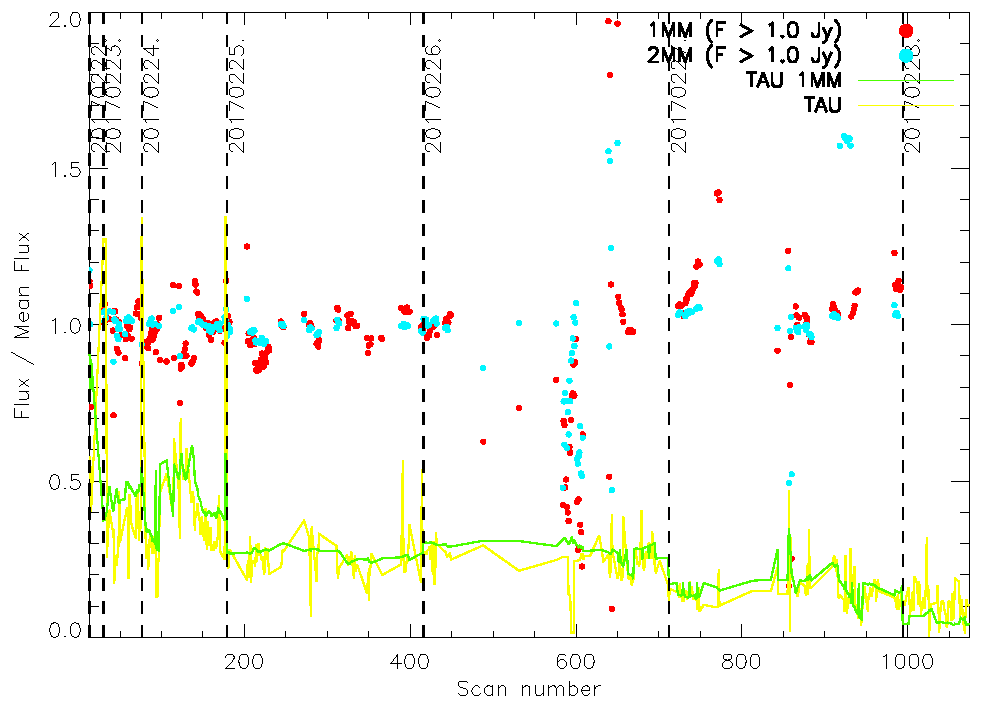
\includegraphics[clip, angle=0, scale = 0.7]{Figures/FluxIndScans/flux_ratio_run22.pdf}
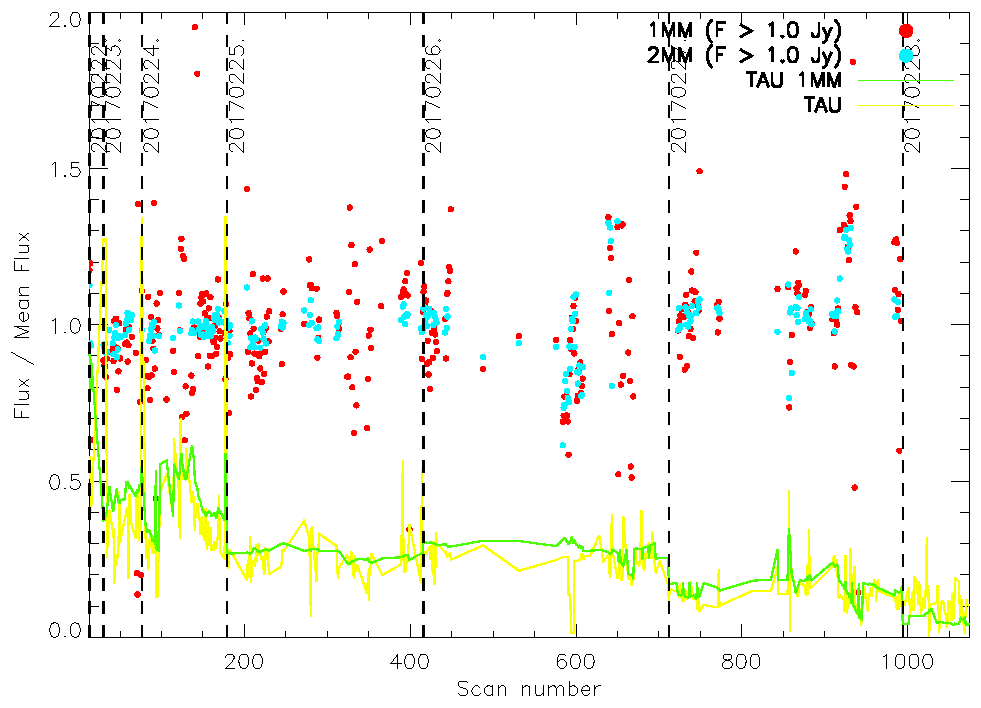
\includegraphics[clip, angle=0, scale = 0.7]{Figures/FluxIndScans/flux_ap_ratio_run22.pdf}
\caption{Ratio between the measured flux per scan and the averaged flux for all sources observed in N2R9. We considered both fixed FWHM (top) and aperture photometry fluxes for the 1 (red) and 2 (cyan) mm channels. }
\label{fig:fluxvsscan}
\end{center}
\end{figure}

\begin{figure}
\begin{center}
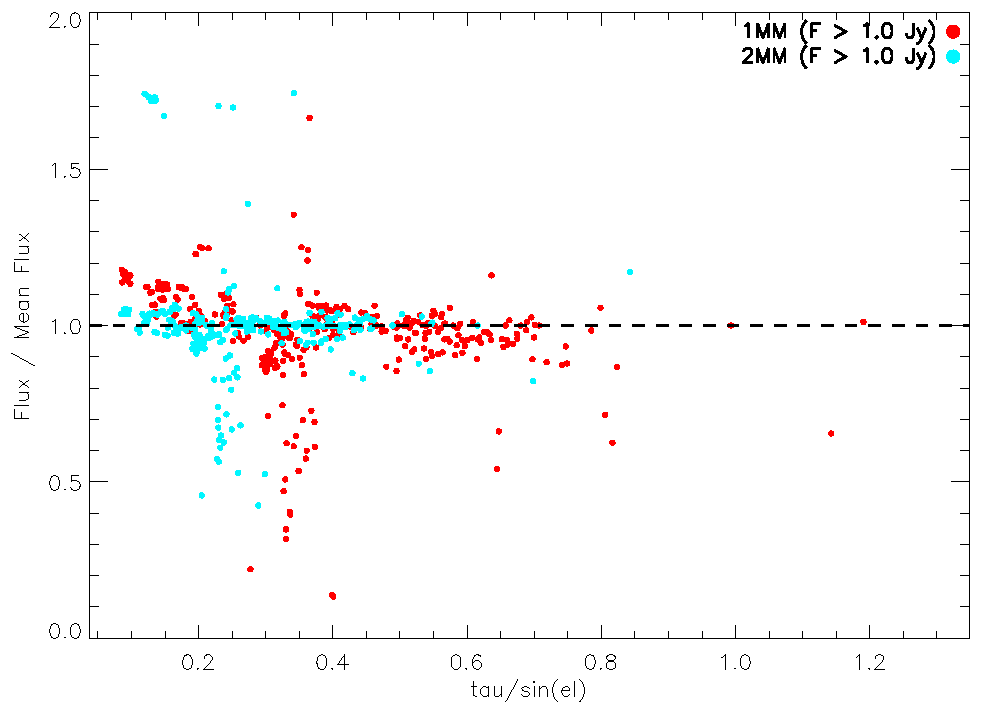
\includegraphics[clip, angle=0, scale = 0.7]{Figures/FluxIndScans/flux_ratio_rz_run22.pdf}
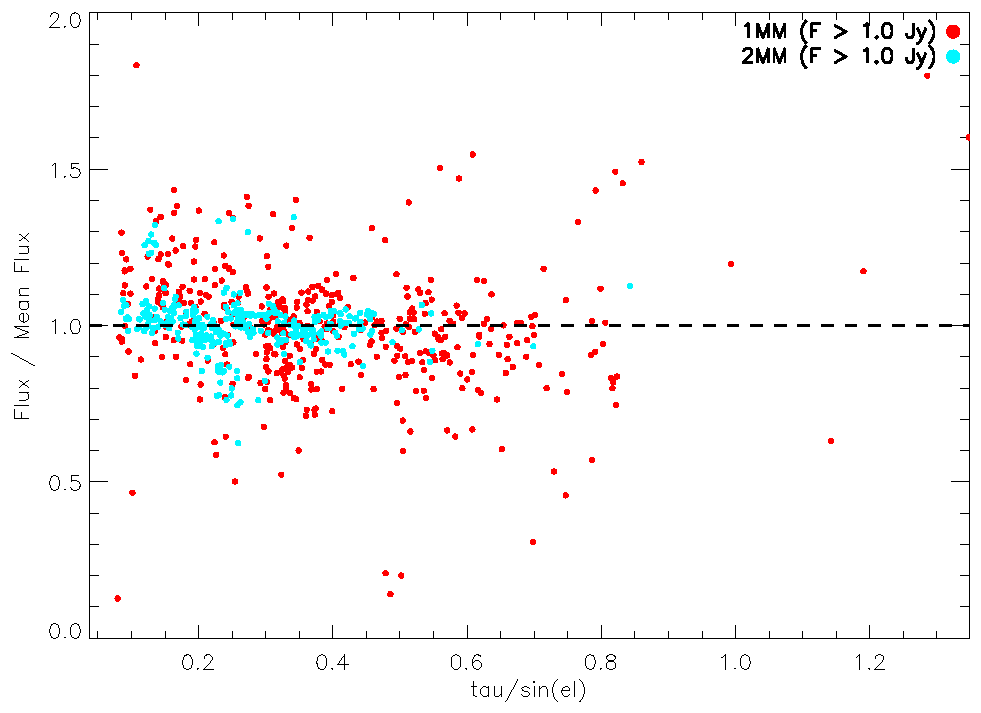
\includegraphics[clip, angle=0, scale = 0.7]{Figures/FluxIndScans/flux_ap_ratio_rz_run22.pdf}
\caption{Ratio between the measured flux per scan and the averaged flux as a function atmospheric backgroud for all sources observed in N2R9. We considered both fixed FWHM (top) and aperture photometry fluxes for the 1 (red) and 2 (cyan) mm channels. }
\label{fig:fluxvsbackground}
\end{center}
\end{figure}



%----------------------------------------------------------------------------------------
%	NOISE DESCRIPTION
%----------------------------------------------------------------------------------------
\section{Noise description: TOI and maps}
\label{se:noise}

\subsection{Dark detectors at 1 mm}
%\begin{figure}
%\begin{center}
%\includegraphics[clip, angle=0, scale = 0.7]{Figures/}
%\includegraphics[clip, angle=0, scale = 0.7]{Figures/FluxIndScans/}
%\caption{ Other stuff}
%\label{fig:fluxvsbackground}
%\end{center}
%\end{figure}


%----------------------------------------------------------------------------------------
%	DARK TESTS
%----------------------------------------------------------------------------------------
\subsection{Dark tests}
\label{se:dark}
\section{Detector-Detector correlation matrix}

For this work we have used several decorrelation methods trying to identify possible multiple components in the noise. Notice that in the following the atmospheric signal will be considered simply as correlated sky noise. The main decorrelation methods used are:

\begin{enumerate}
\item[CM] {\bf Common mode decorrelation}. We search for a common mode template using all detectors of the same array. To avoid bias from bad detectors we consider the median common mode.

\item[PCA] {\bf Principal Component Analysis}. For each NIKA2 array independently we decompose the covariance matrix in principal components. From those we derive up to 10 independent templates corresponding to the largest eigenvalue values.

\item[BC] {\bf Best correlated pixels}. For each detector in a given array we identify those detectors which are more correlated to it (a minimum of 14). Using those detectors we compute a common mode as in method CM. 

\item[ALL] {\bf All detectors}. For earch detector of a given array we use all other detectors of the same array as templates and perform a linear fit.

\end{enumerate}

We present in Figure~\ref{corrs299} the detector noise correlation matrices computed for the N2R7 dark scan 20161211s299 for the three arrays (A1, A2, and A3 from left to right). From top to bottom we present the correlation matrices for the raw data (no decorrelation), and for the CM, PCA, and BC decorrelated data. For each array the extent and name (from letter A to T) of the electronic boxes is indicated on the left of the figure. Notice that each electronic box consists of 5 subbands. \\

In the case of the raw data we observe very different structures for the three arrays. In arrays A1 and A2, we observe significant structure going from very correlated detectors to fully uncorrelated ones. This is observed even within a given electronic box or even between detectors from the same electronic subband. By contrast in A3 the detectors seems to be fully correlated. After CM decorrelation we observe that there is still significant correlation and anti-correlation for some detectors. In particular we observe a very clear pattern in A2 for electronic box A. In the case of the PCA decorrelated data the correlation matrix becomes much more diagonal although still shows significant level correlation within electronic subbands. We also notice that using the BC decorrelation improves with respect to the CM decorrelation but it is worse than the PCA case. These results tends indicate various electronic or detector related noise components. \\

In Figure~\ref{corrs72} we show the noise correlation matrices for the N2R7 faint source scan 20161213s72. As expected the raw data noise correlation is dominated by atmospheric noise and we observe full correlation between detectors. After decorrelation the results are very similar to those found for N2R7 dark scan 20161211s299. There is residual significant correlation and anti-correlation after CM decorrelation. PCA decorrelation leads to a more diagonal correlation matrices. For the BC decorrelation the results are worse (more residual correlation and anti-correlation) and close to those of the CM decorrelation. As before there are good indications of multiple electronic-detector noise components. It is interesting to note that the detector-electronic noise correlation patterns seems to be the same for dark tests and for sky data. 

We have repeated the same analysis on scans of the N2R4 both for dark tests, scan 20160504s97, and faint sources, scan 20160313s87. We find few significant differences with respect to previoius results. In the case of the dark test and for the raw data, the A1 and A2 detectors seems to be more correlated. Furthermore A2 show more significant correlation after CM decorrelation for electronic boxes B and D. Array A1 show also significant residual correlation and anti-correlation after CM et BC decorrelations. For the faint source N2R4 scan 
20160313s87 we observe similar behavior but the pattern of the correlation matrices are not the same that for the dark test scan.

\begin{figure}[ht] % Inline image example
\begin{center}
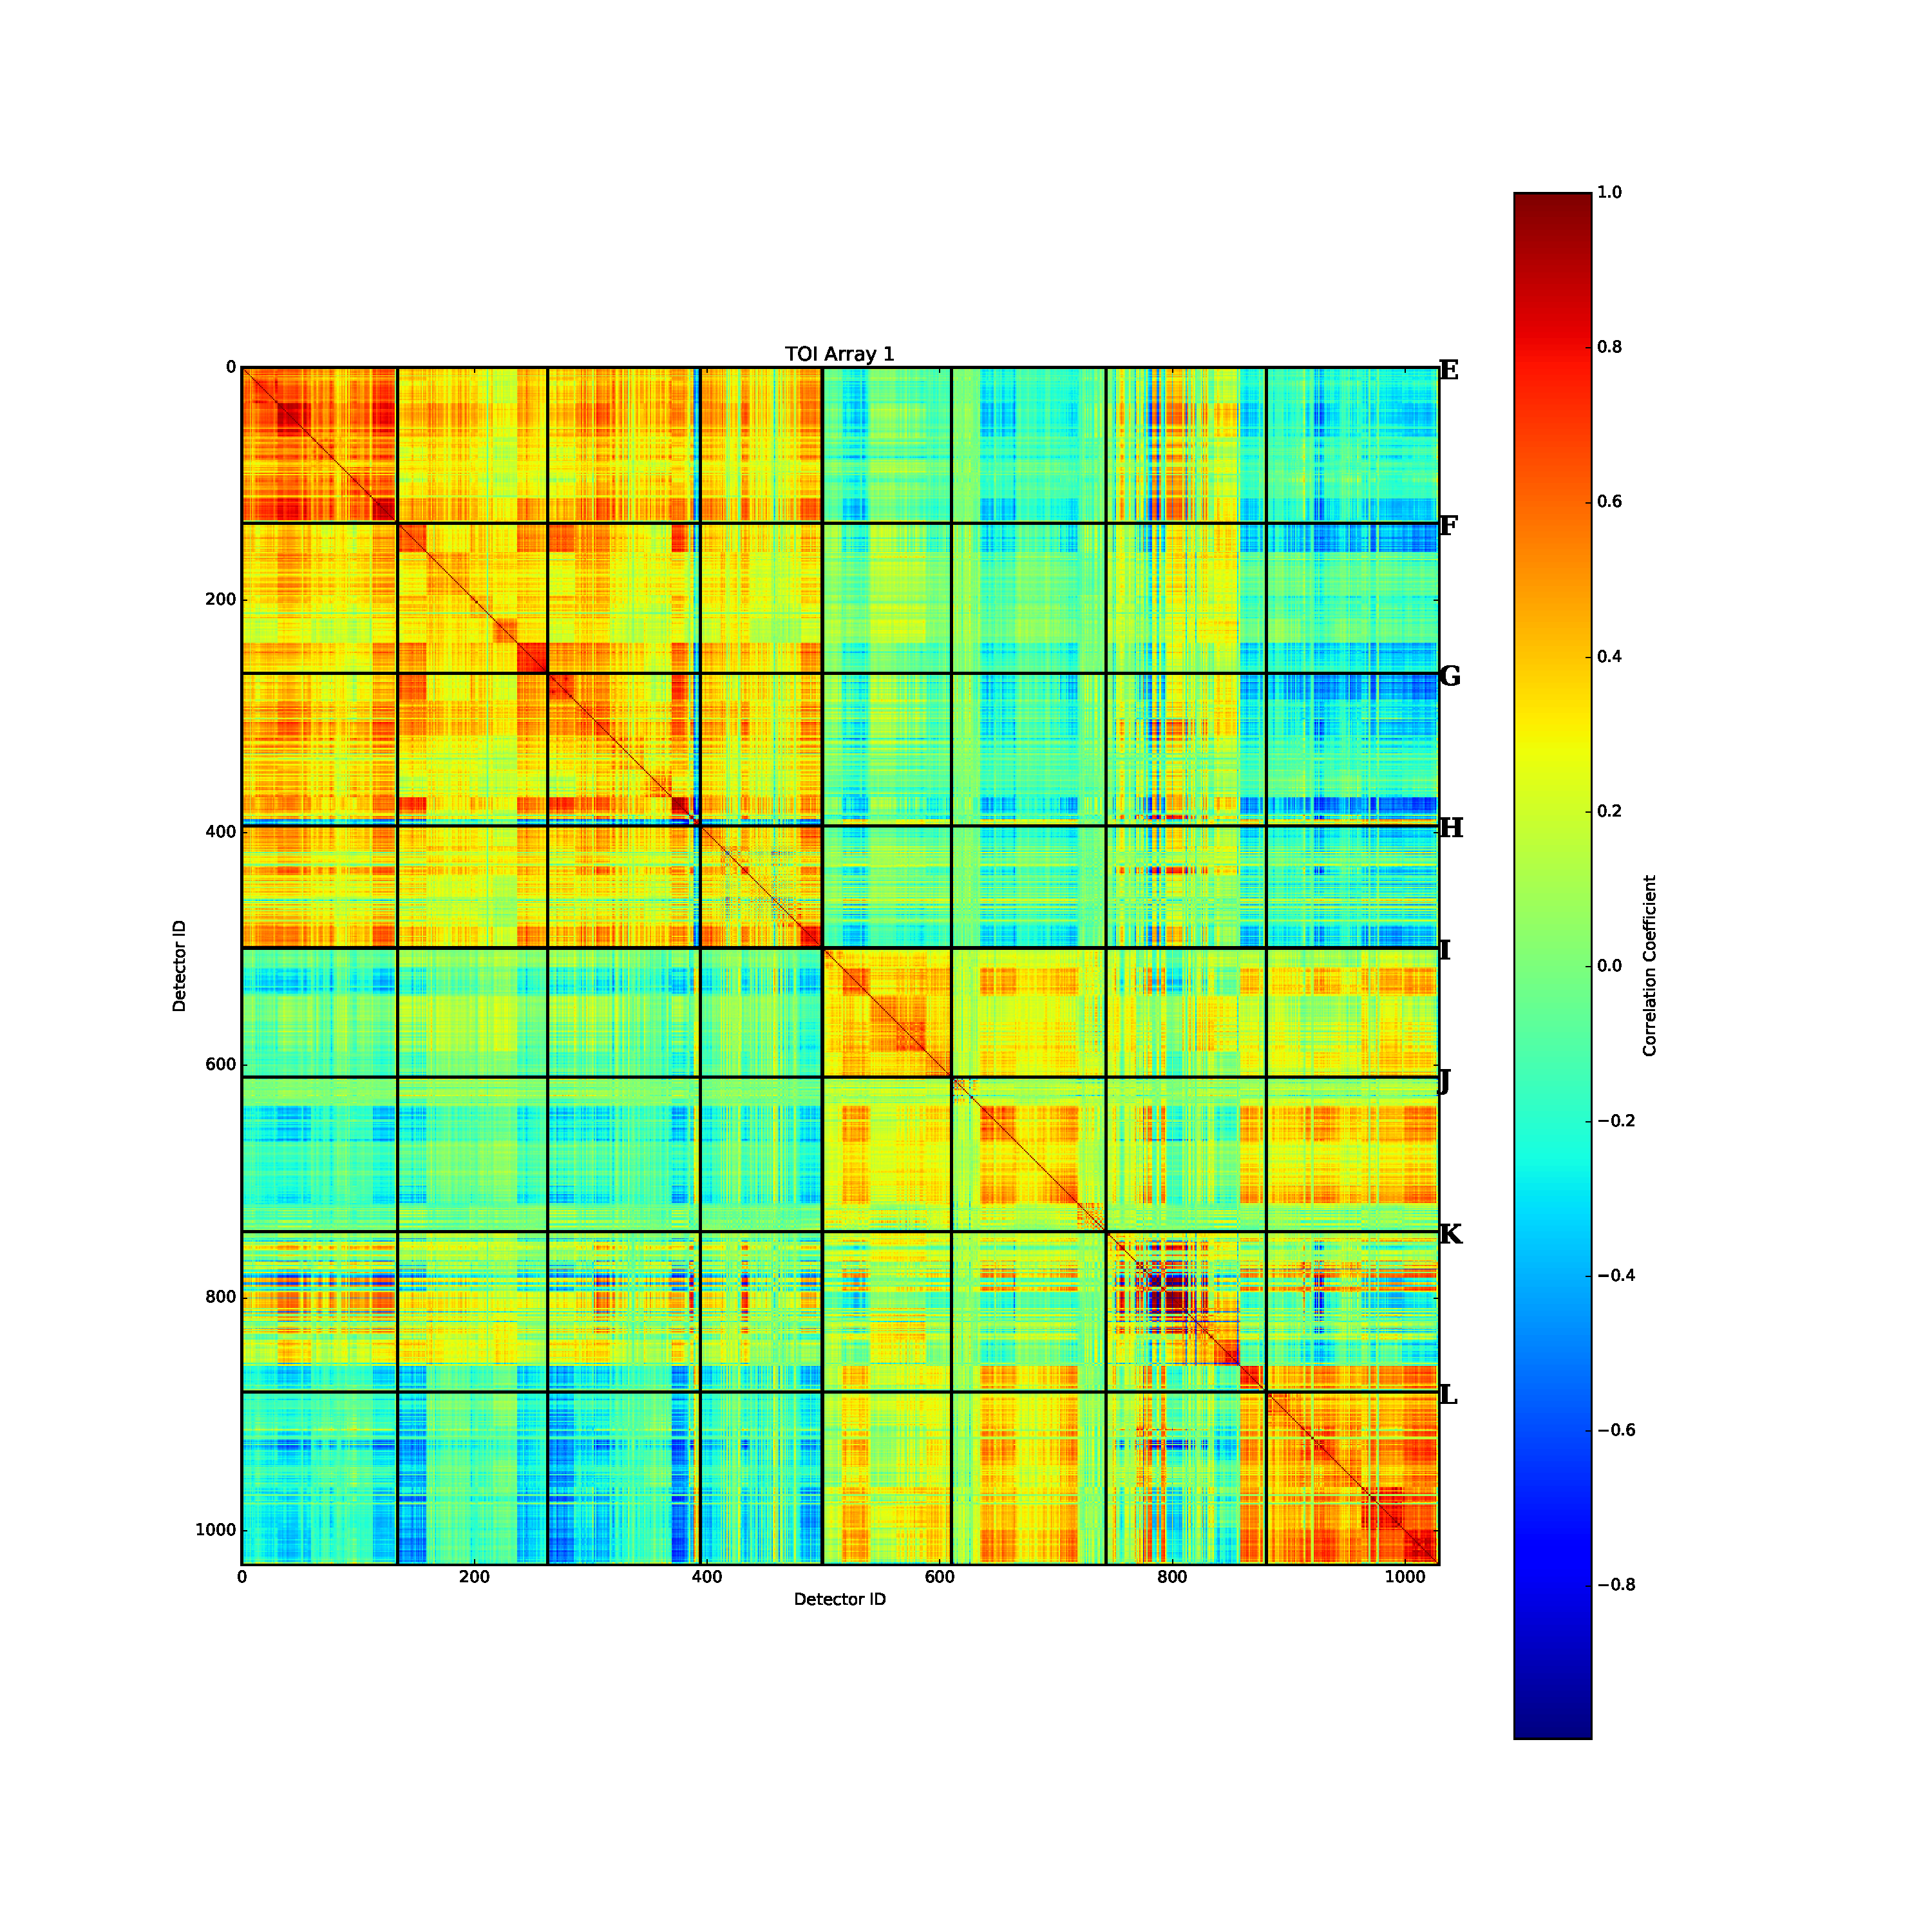
\includegraphics[width=0.3\textwidth]{Figures/DarkTests/corrmat_TOI_array_1_20161211s299.pdf}
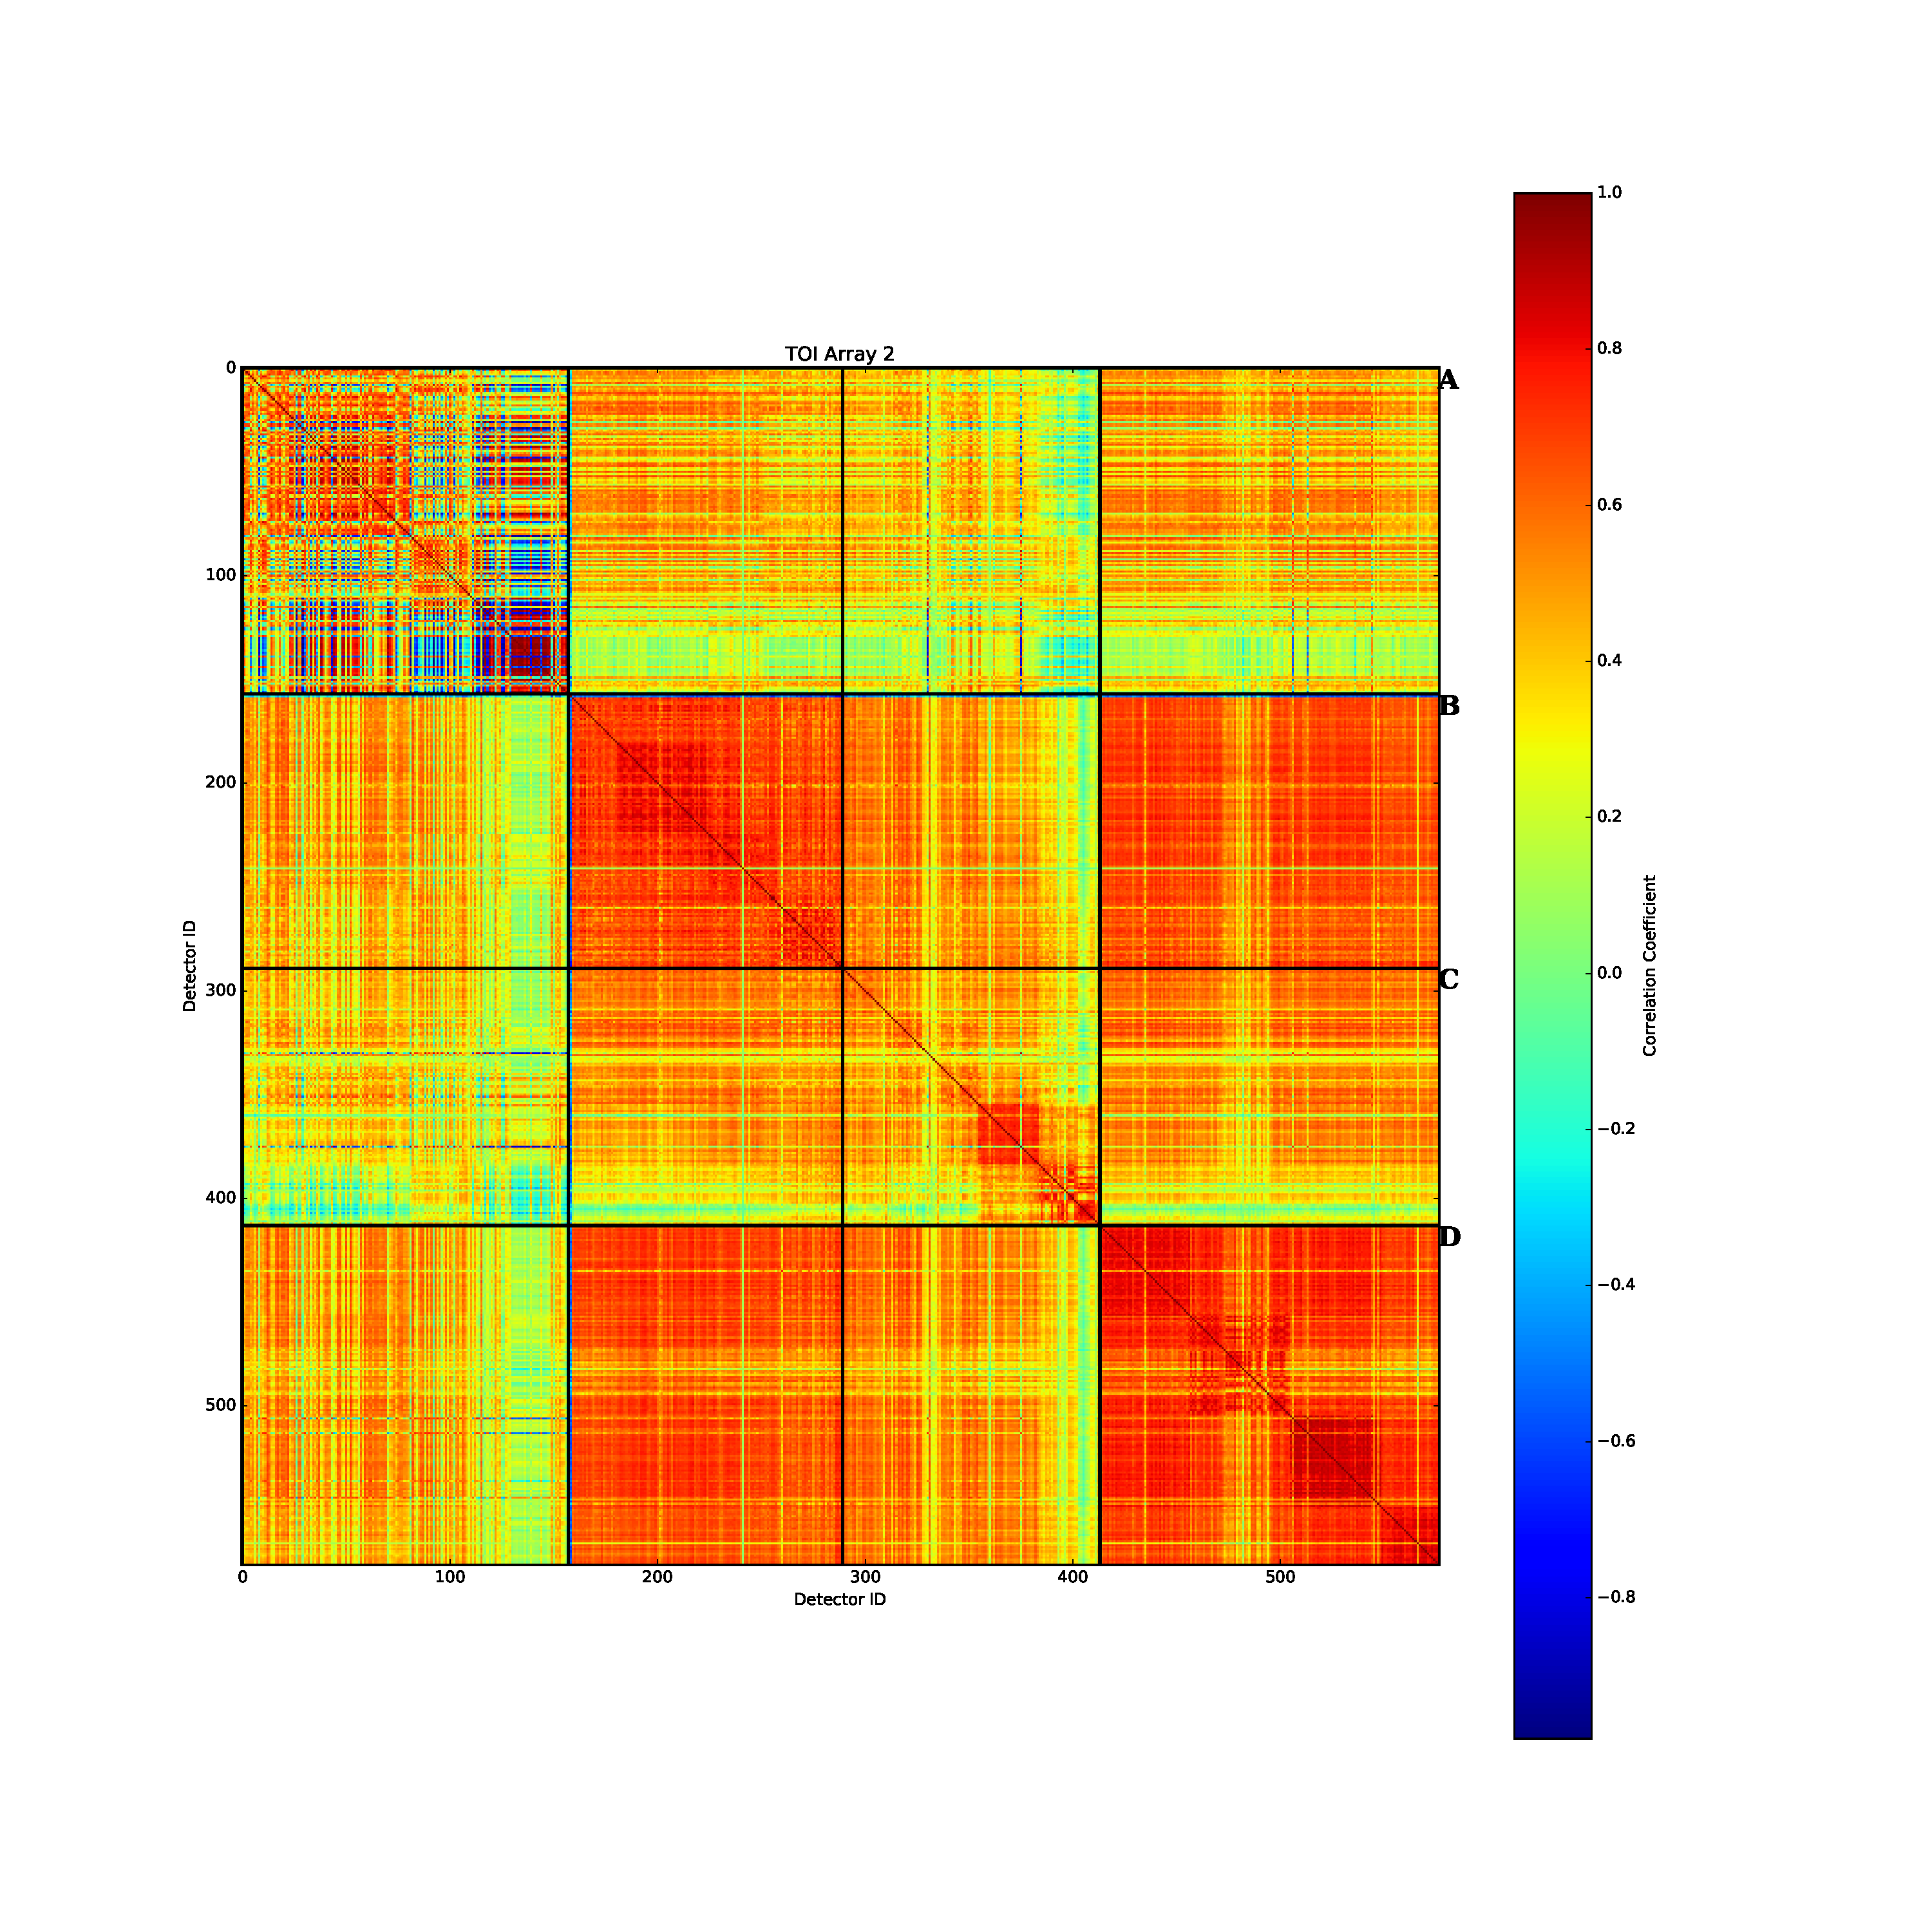
\includegraphics[width=0.3\textwidth]{Figures/DarkTests/corrmat_TOI_array_2_20161211s299.pdf}
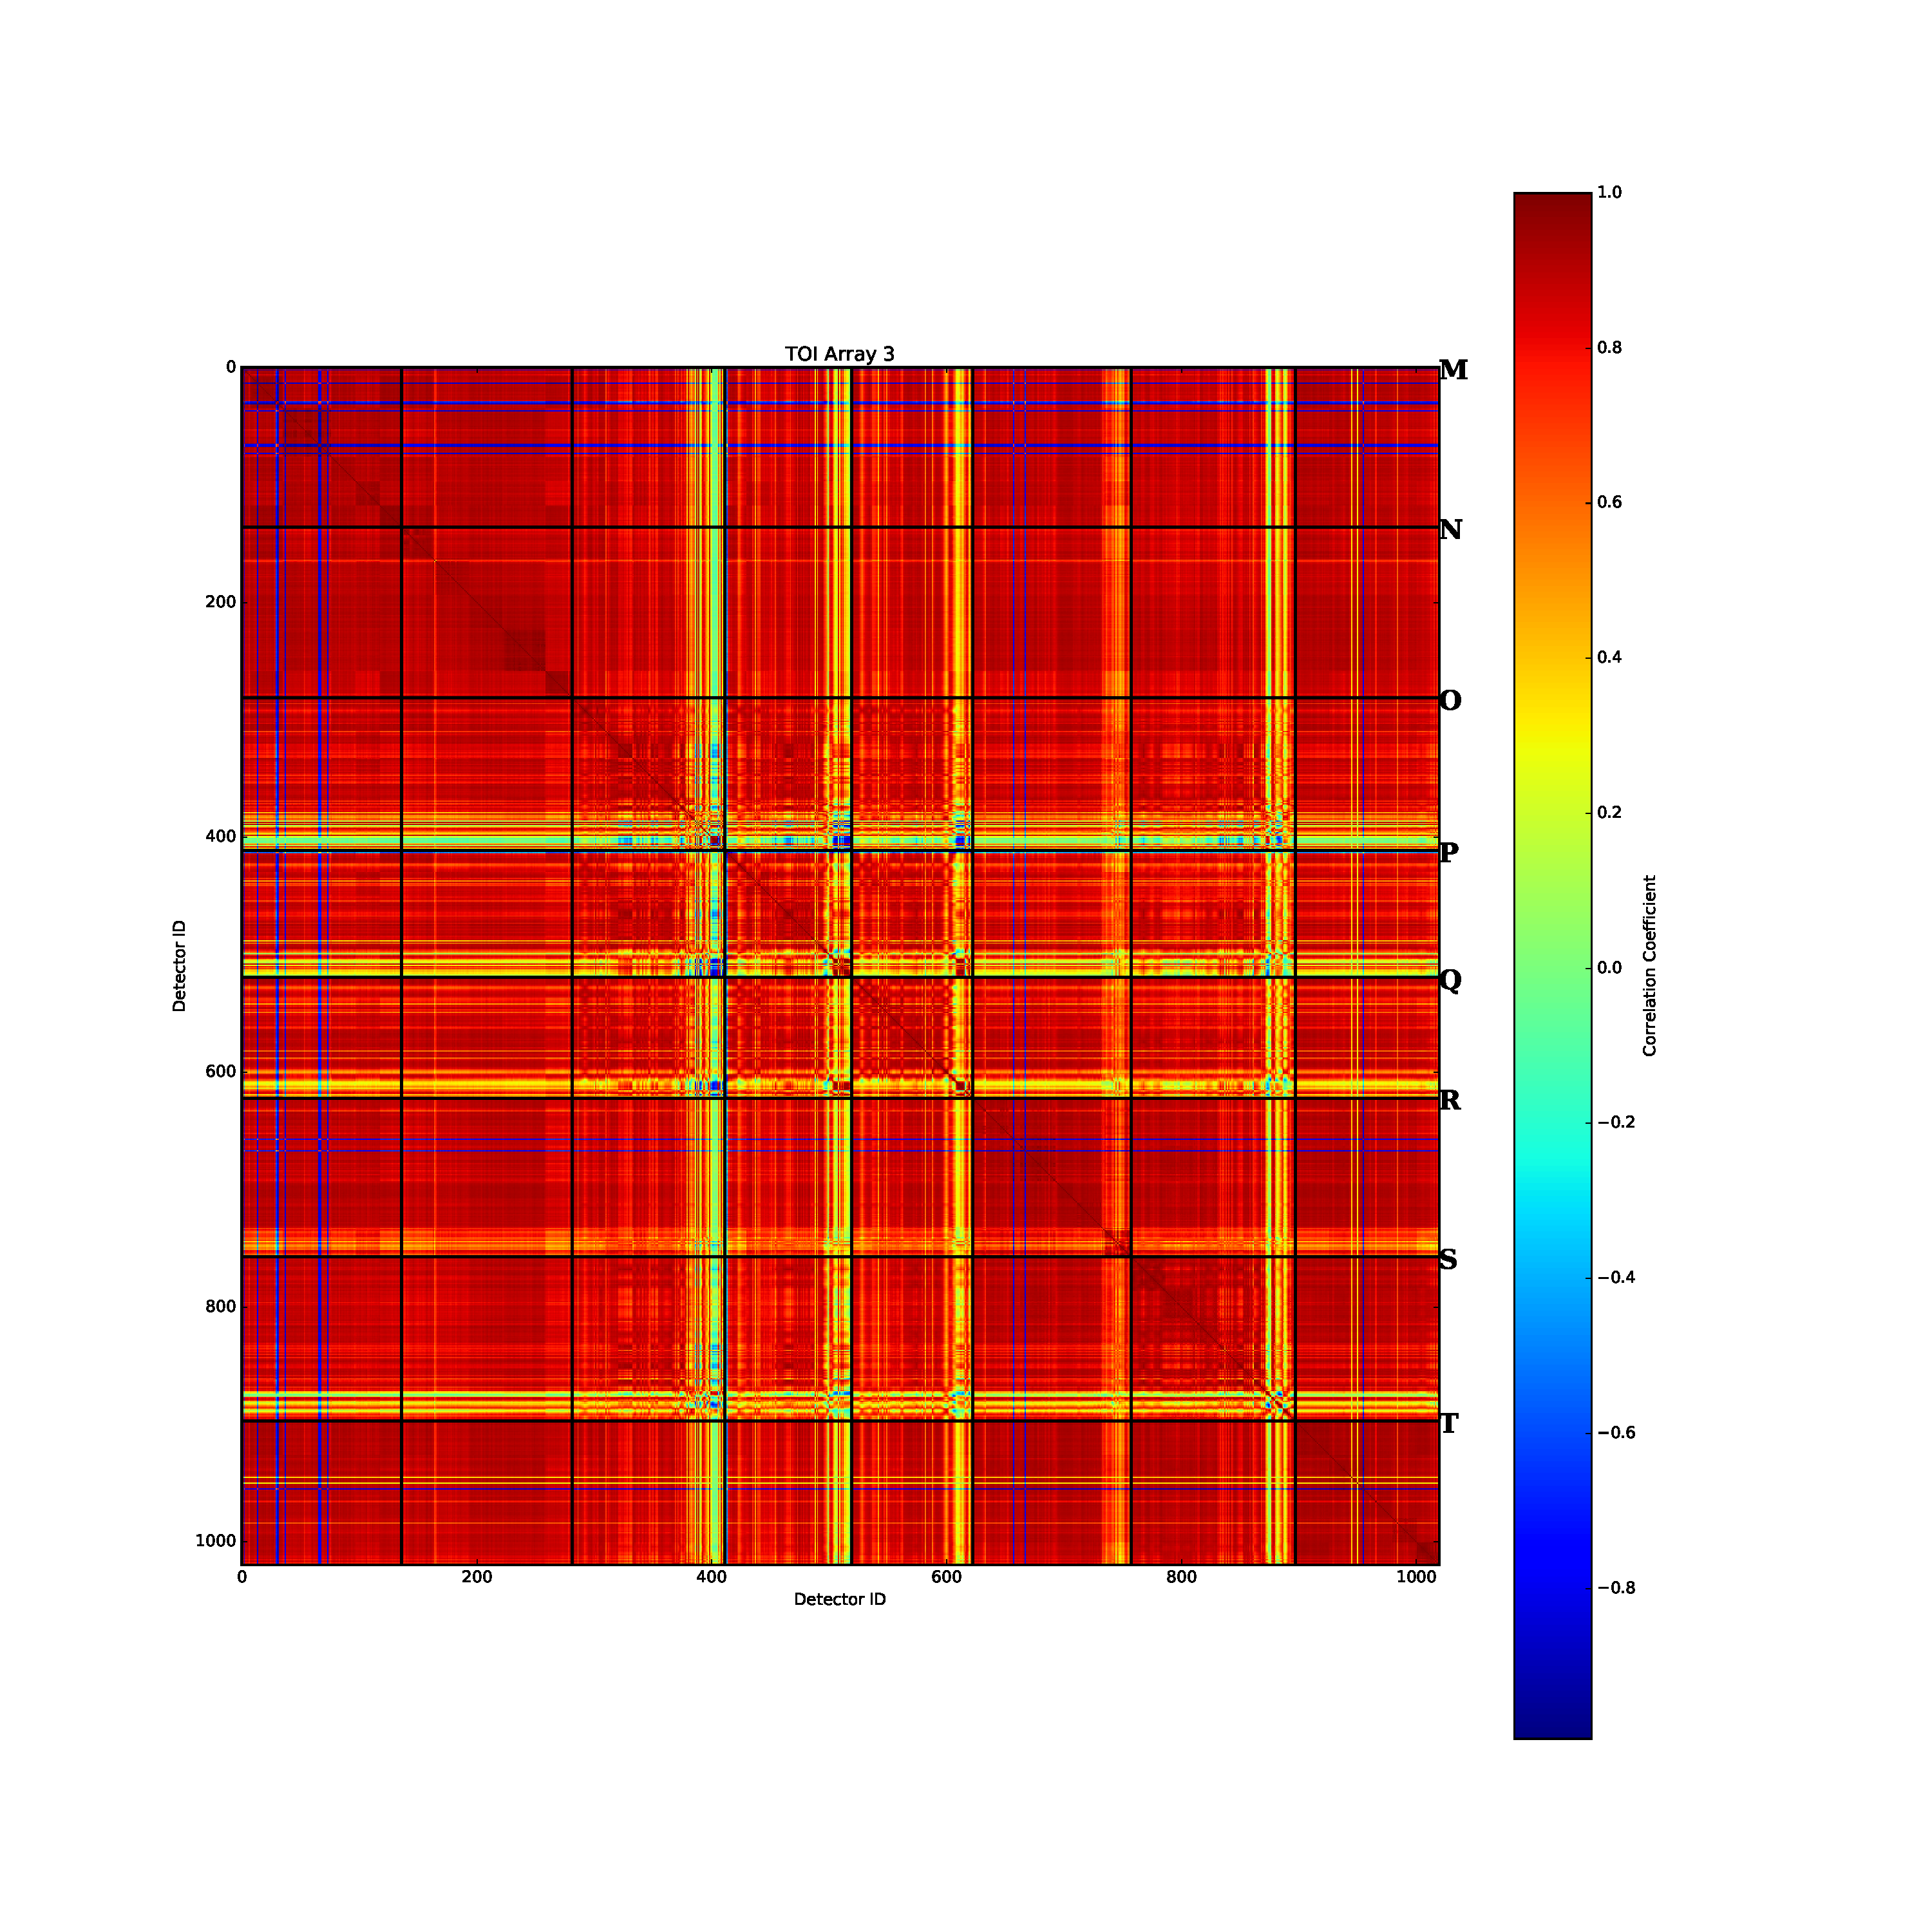
\includegraphics[width=0.3\textwidth]{Figures/DarkTests/corrmat_TOI_array_3_20161211s299.pdf}
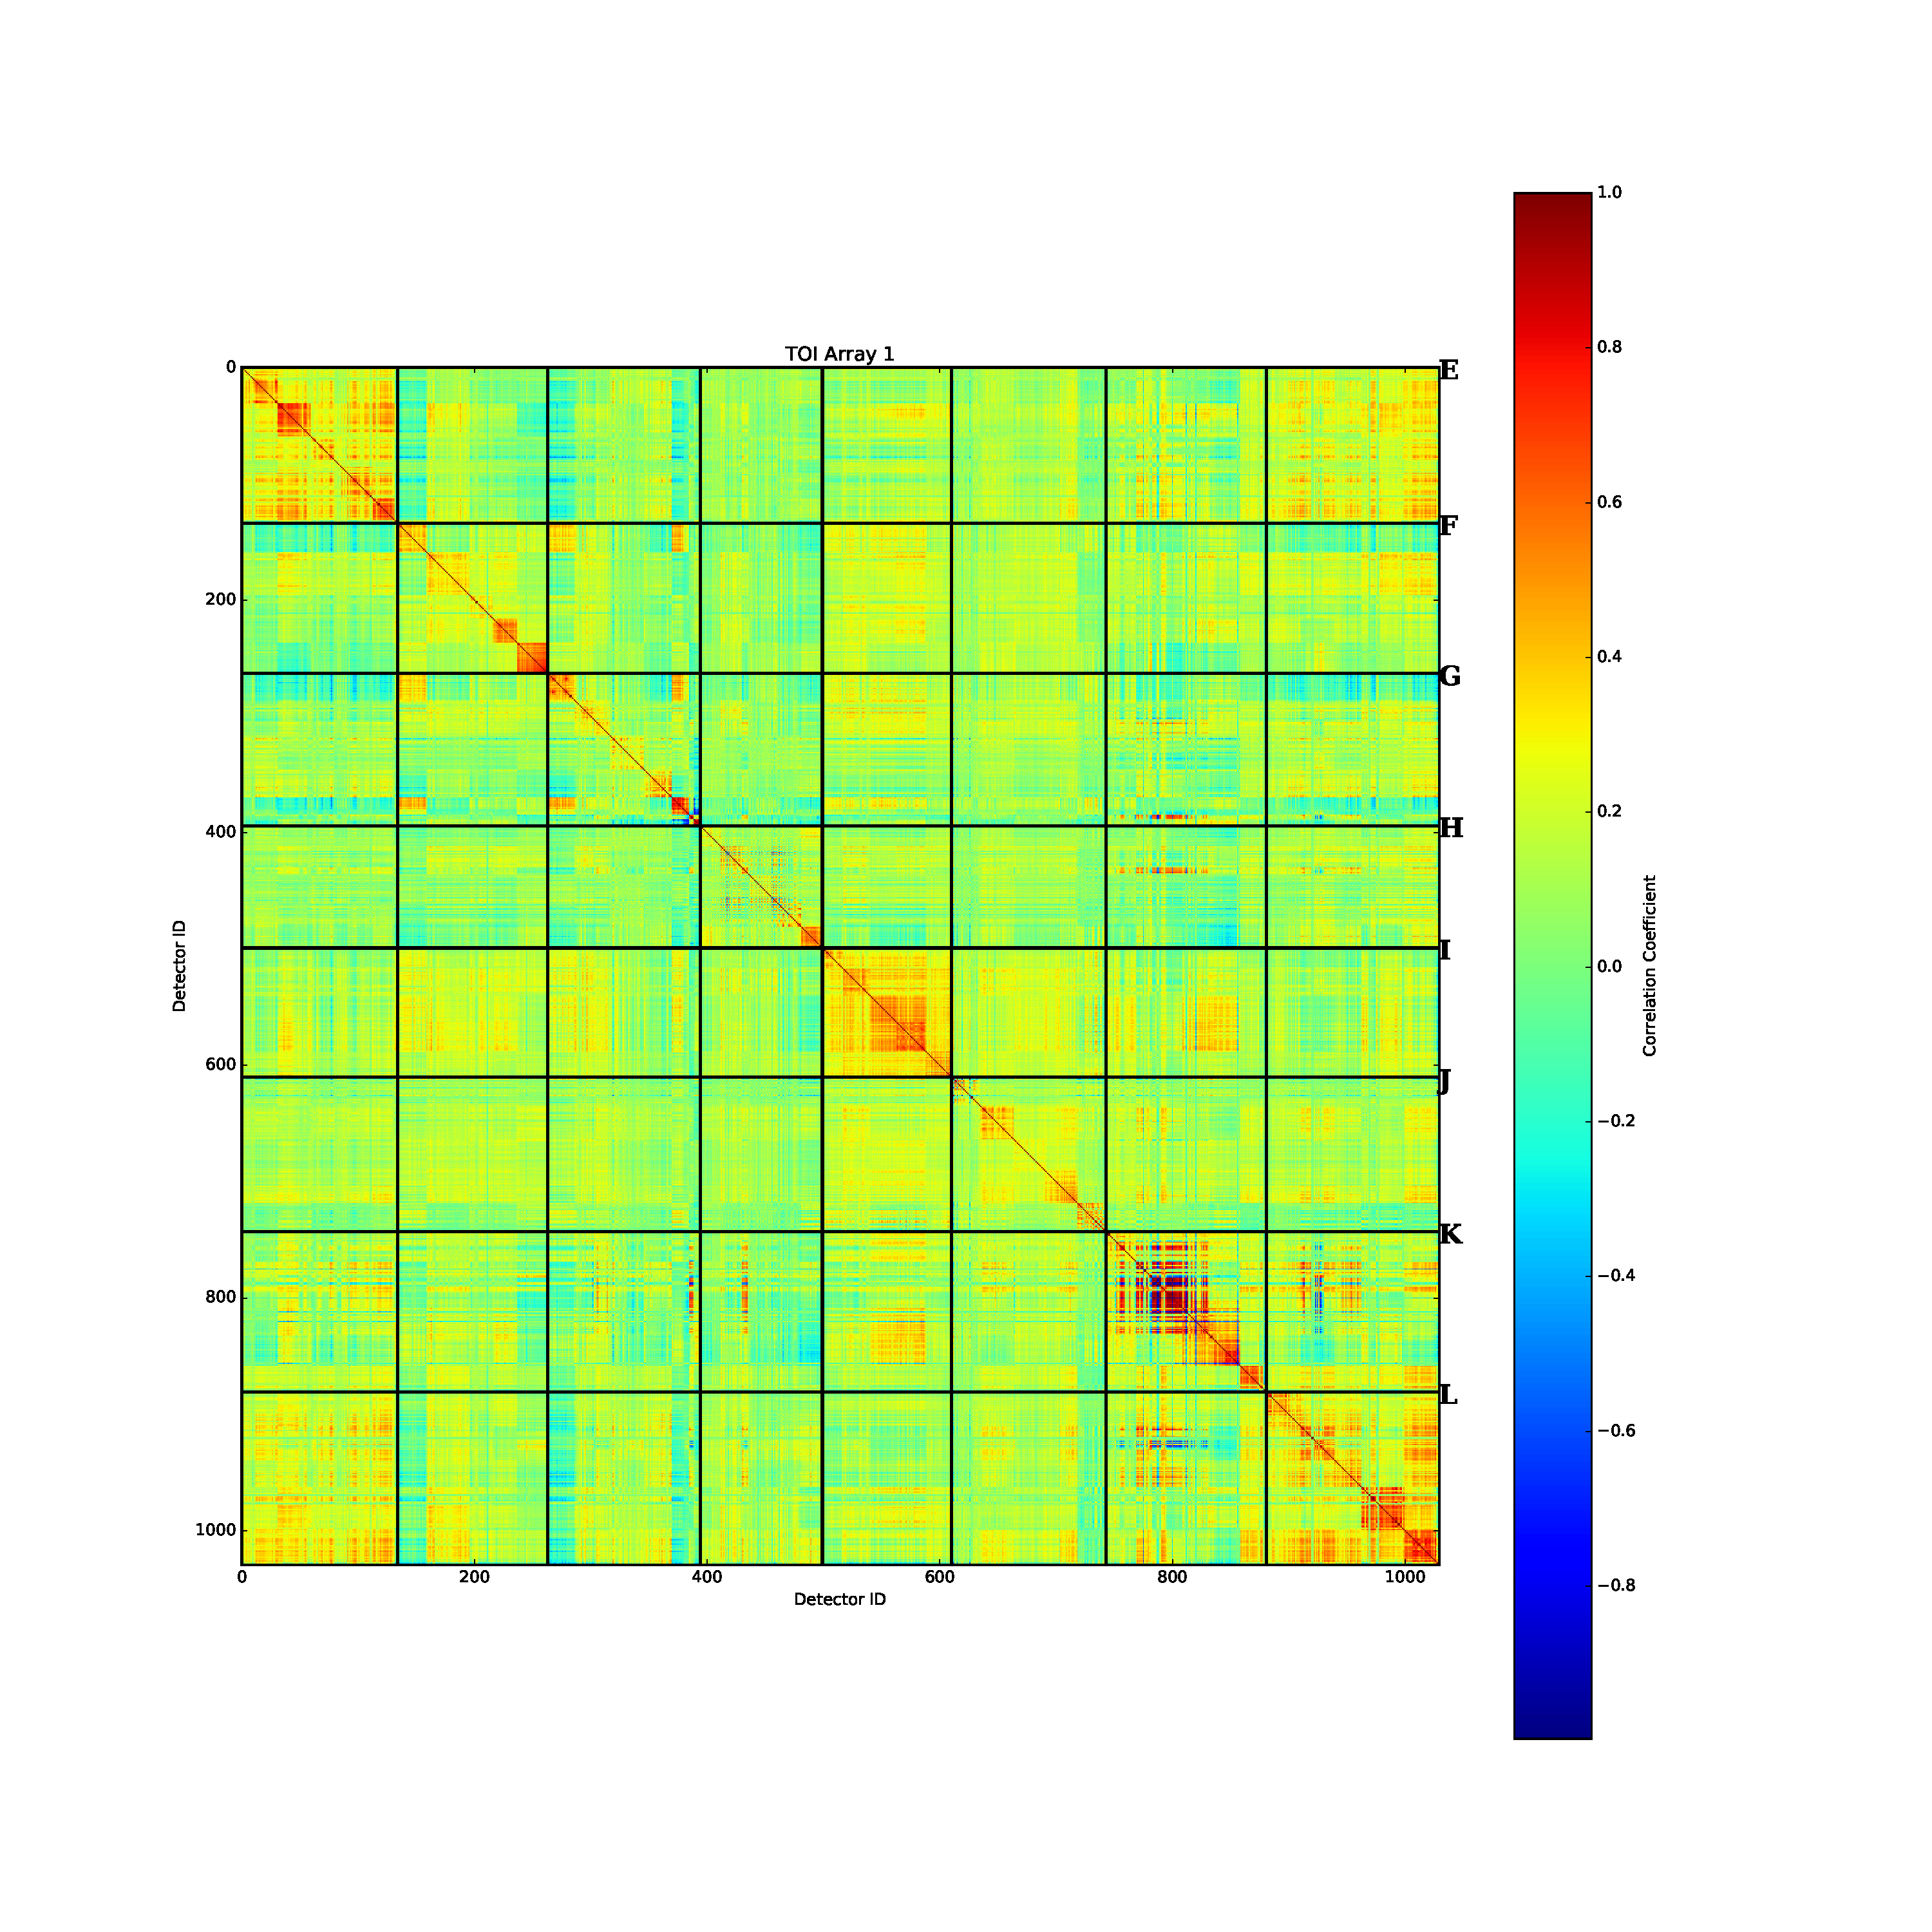
\includegraphics[width=0.3\textwidth]{Figures/DarkTests/corrmat_TOI_CM_array_1_20161211s299.pdf}
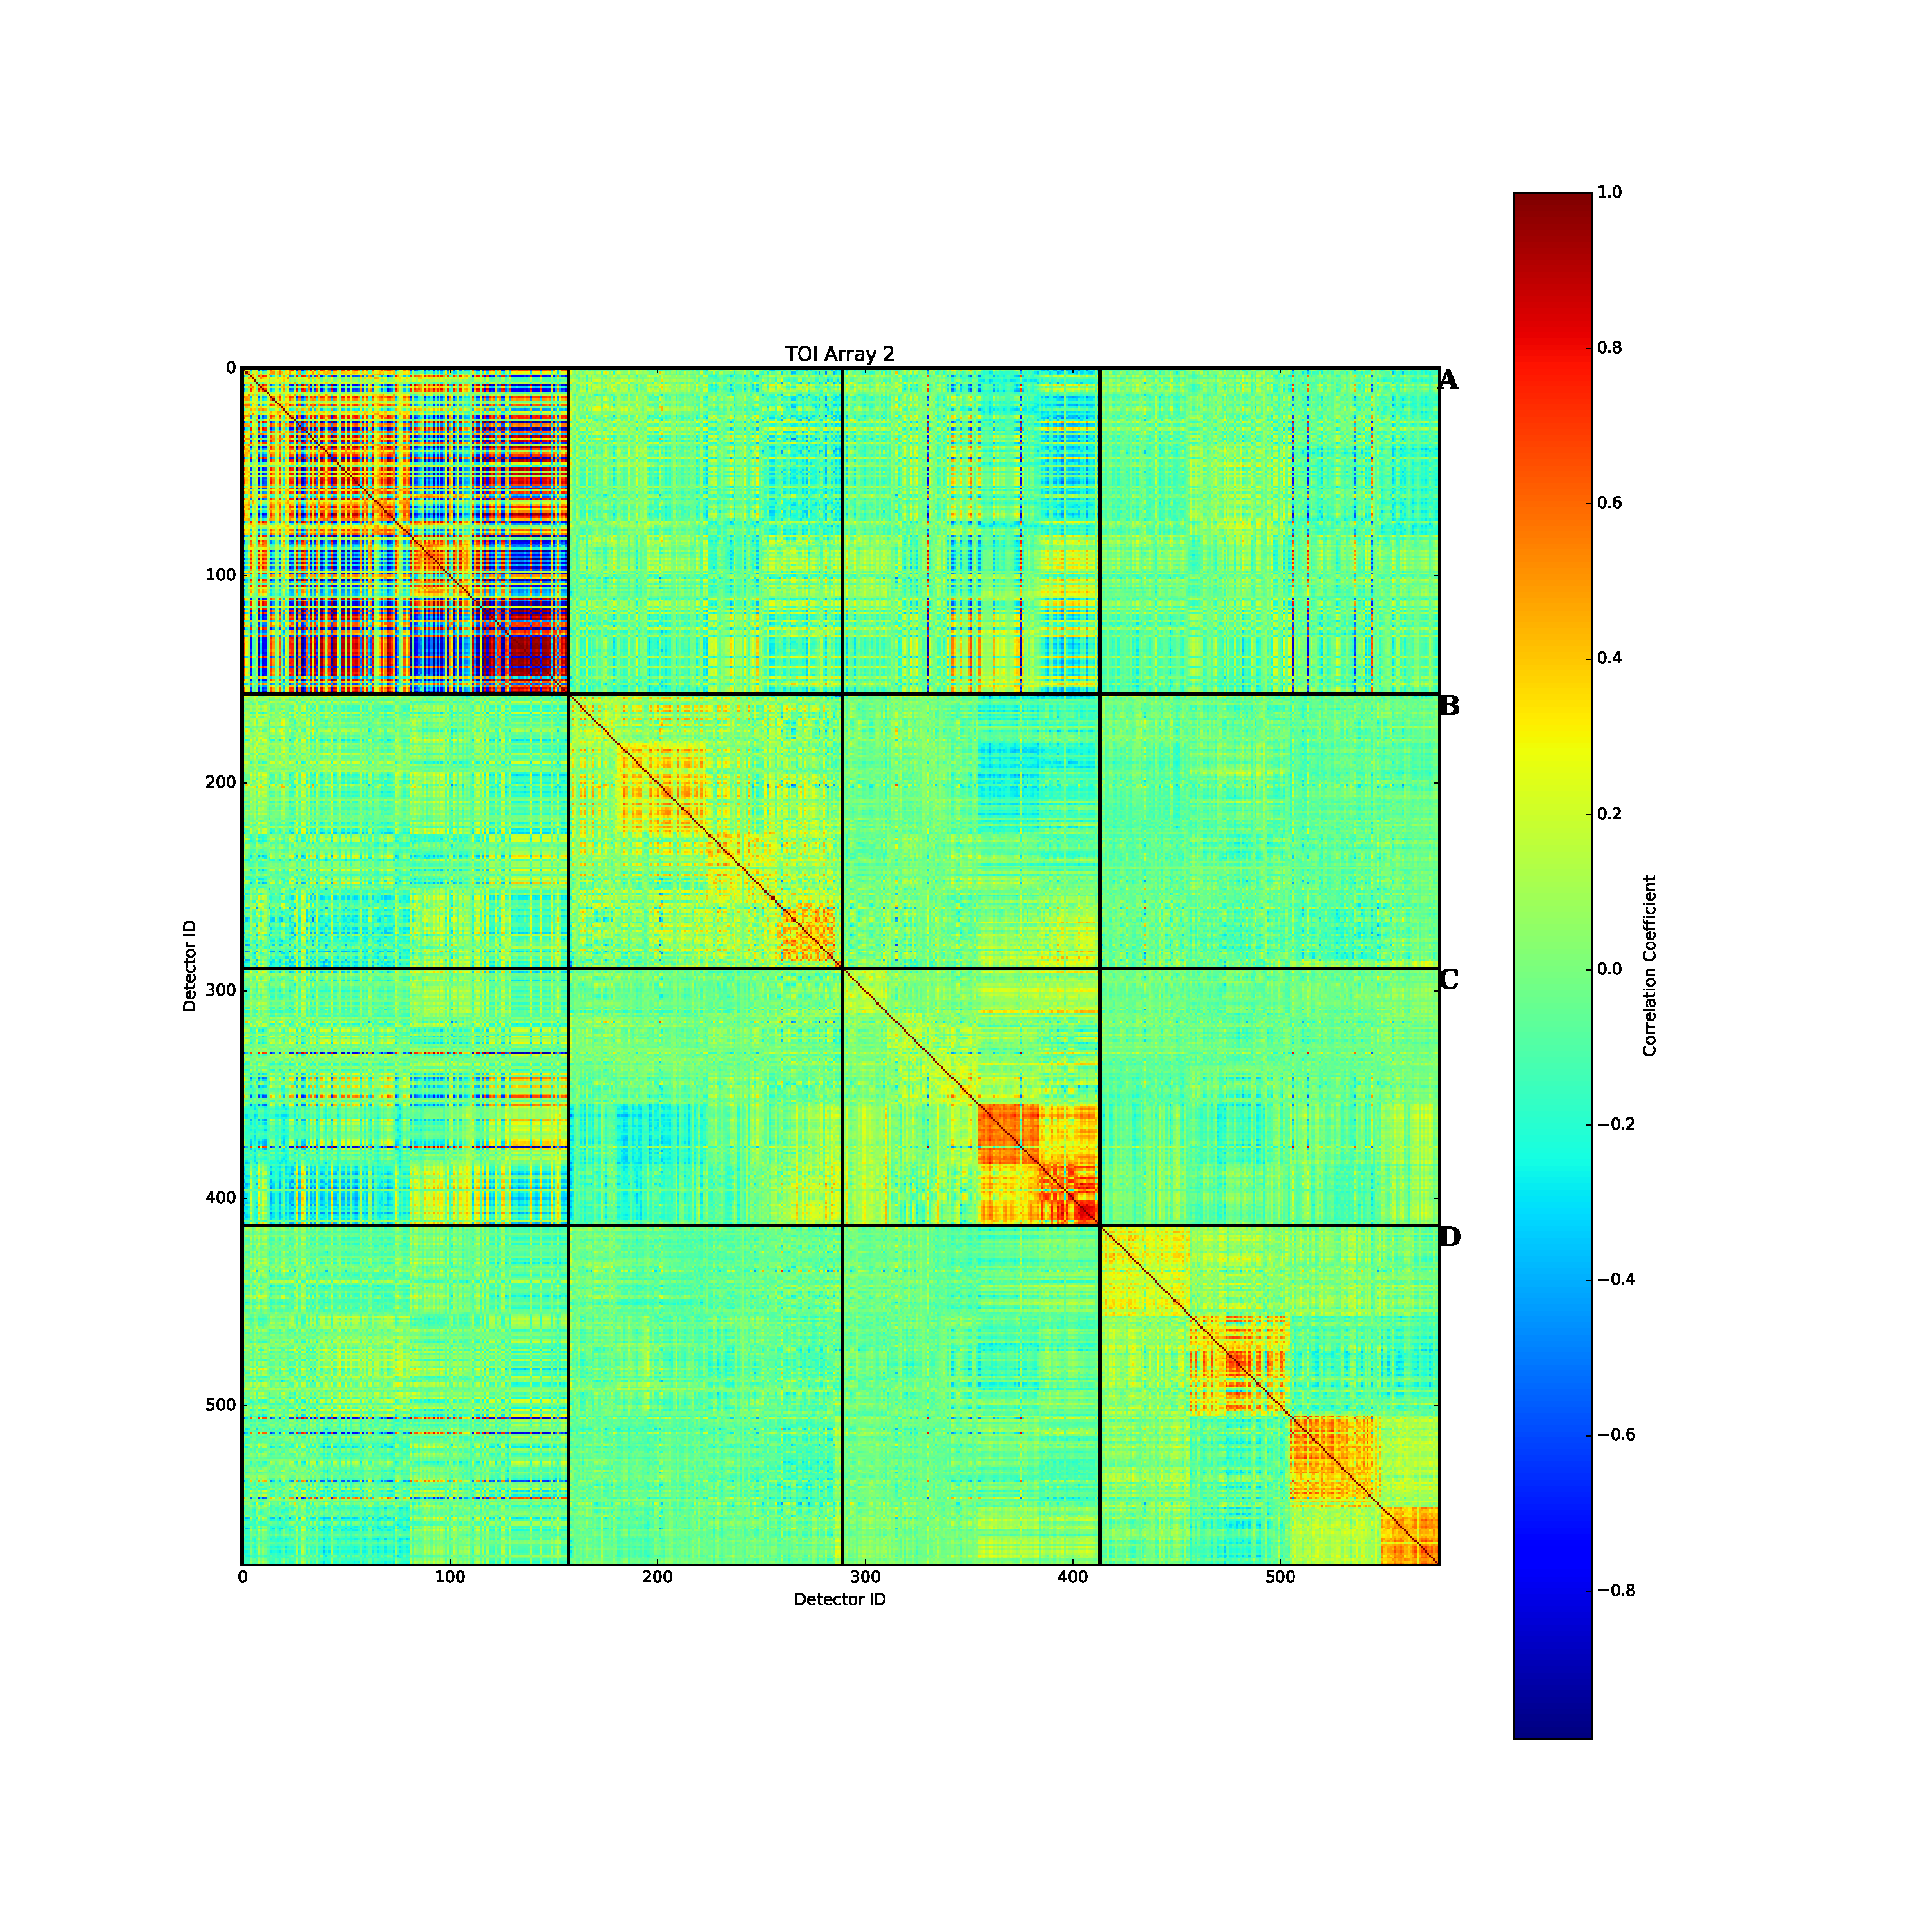
\includegraphics[width=0.3\textwidth]{Figures/DarkTests/corrmat_TOI_CM_array_2_20161211s299.pdf}
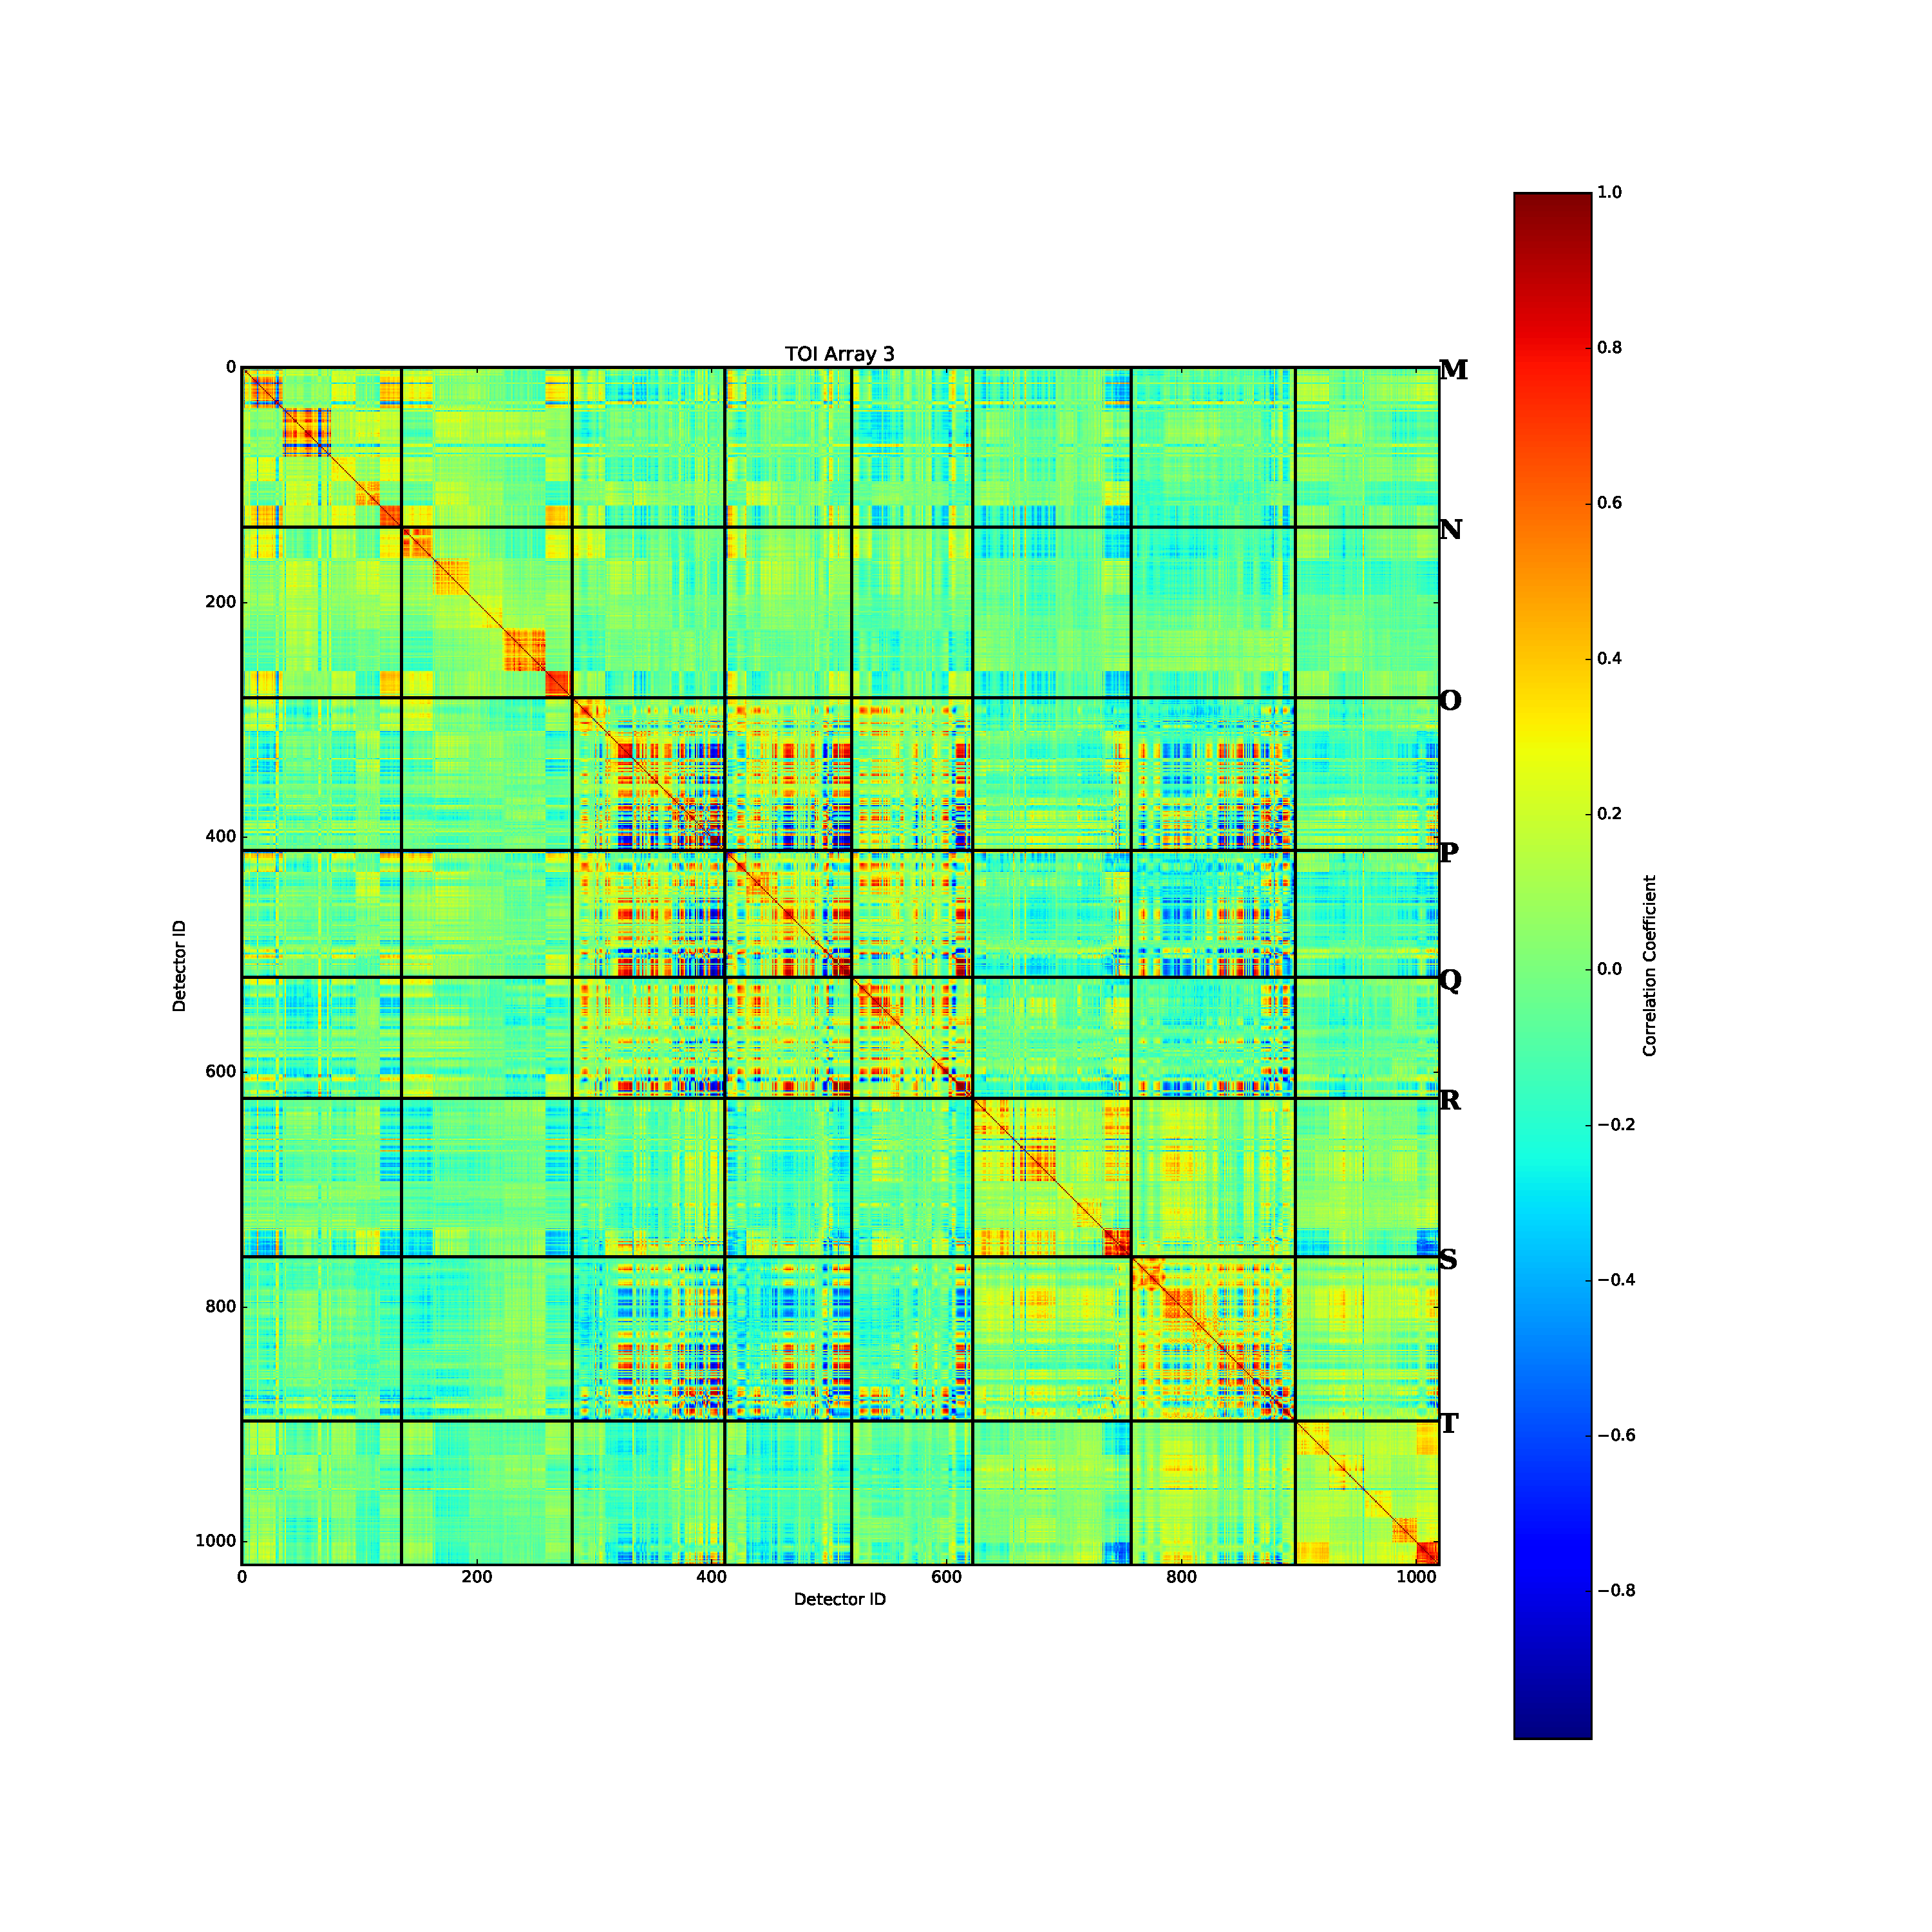
\includegraphics[width=0.3\textwidth]{Figures/DarkTests/corrmat_TOI_CM_array_3_20161211s299.pdf}
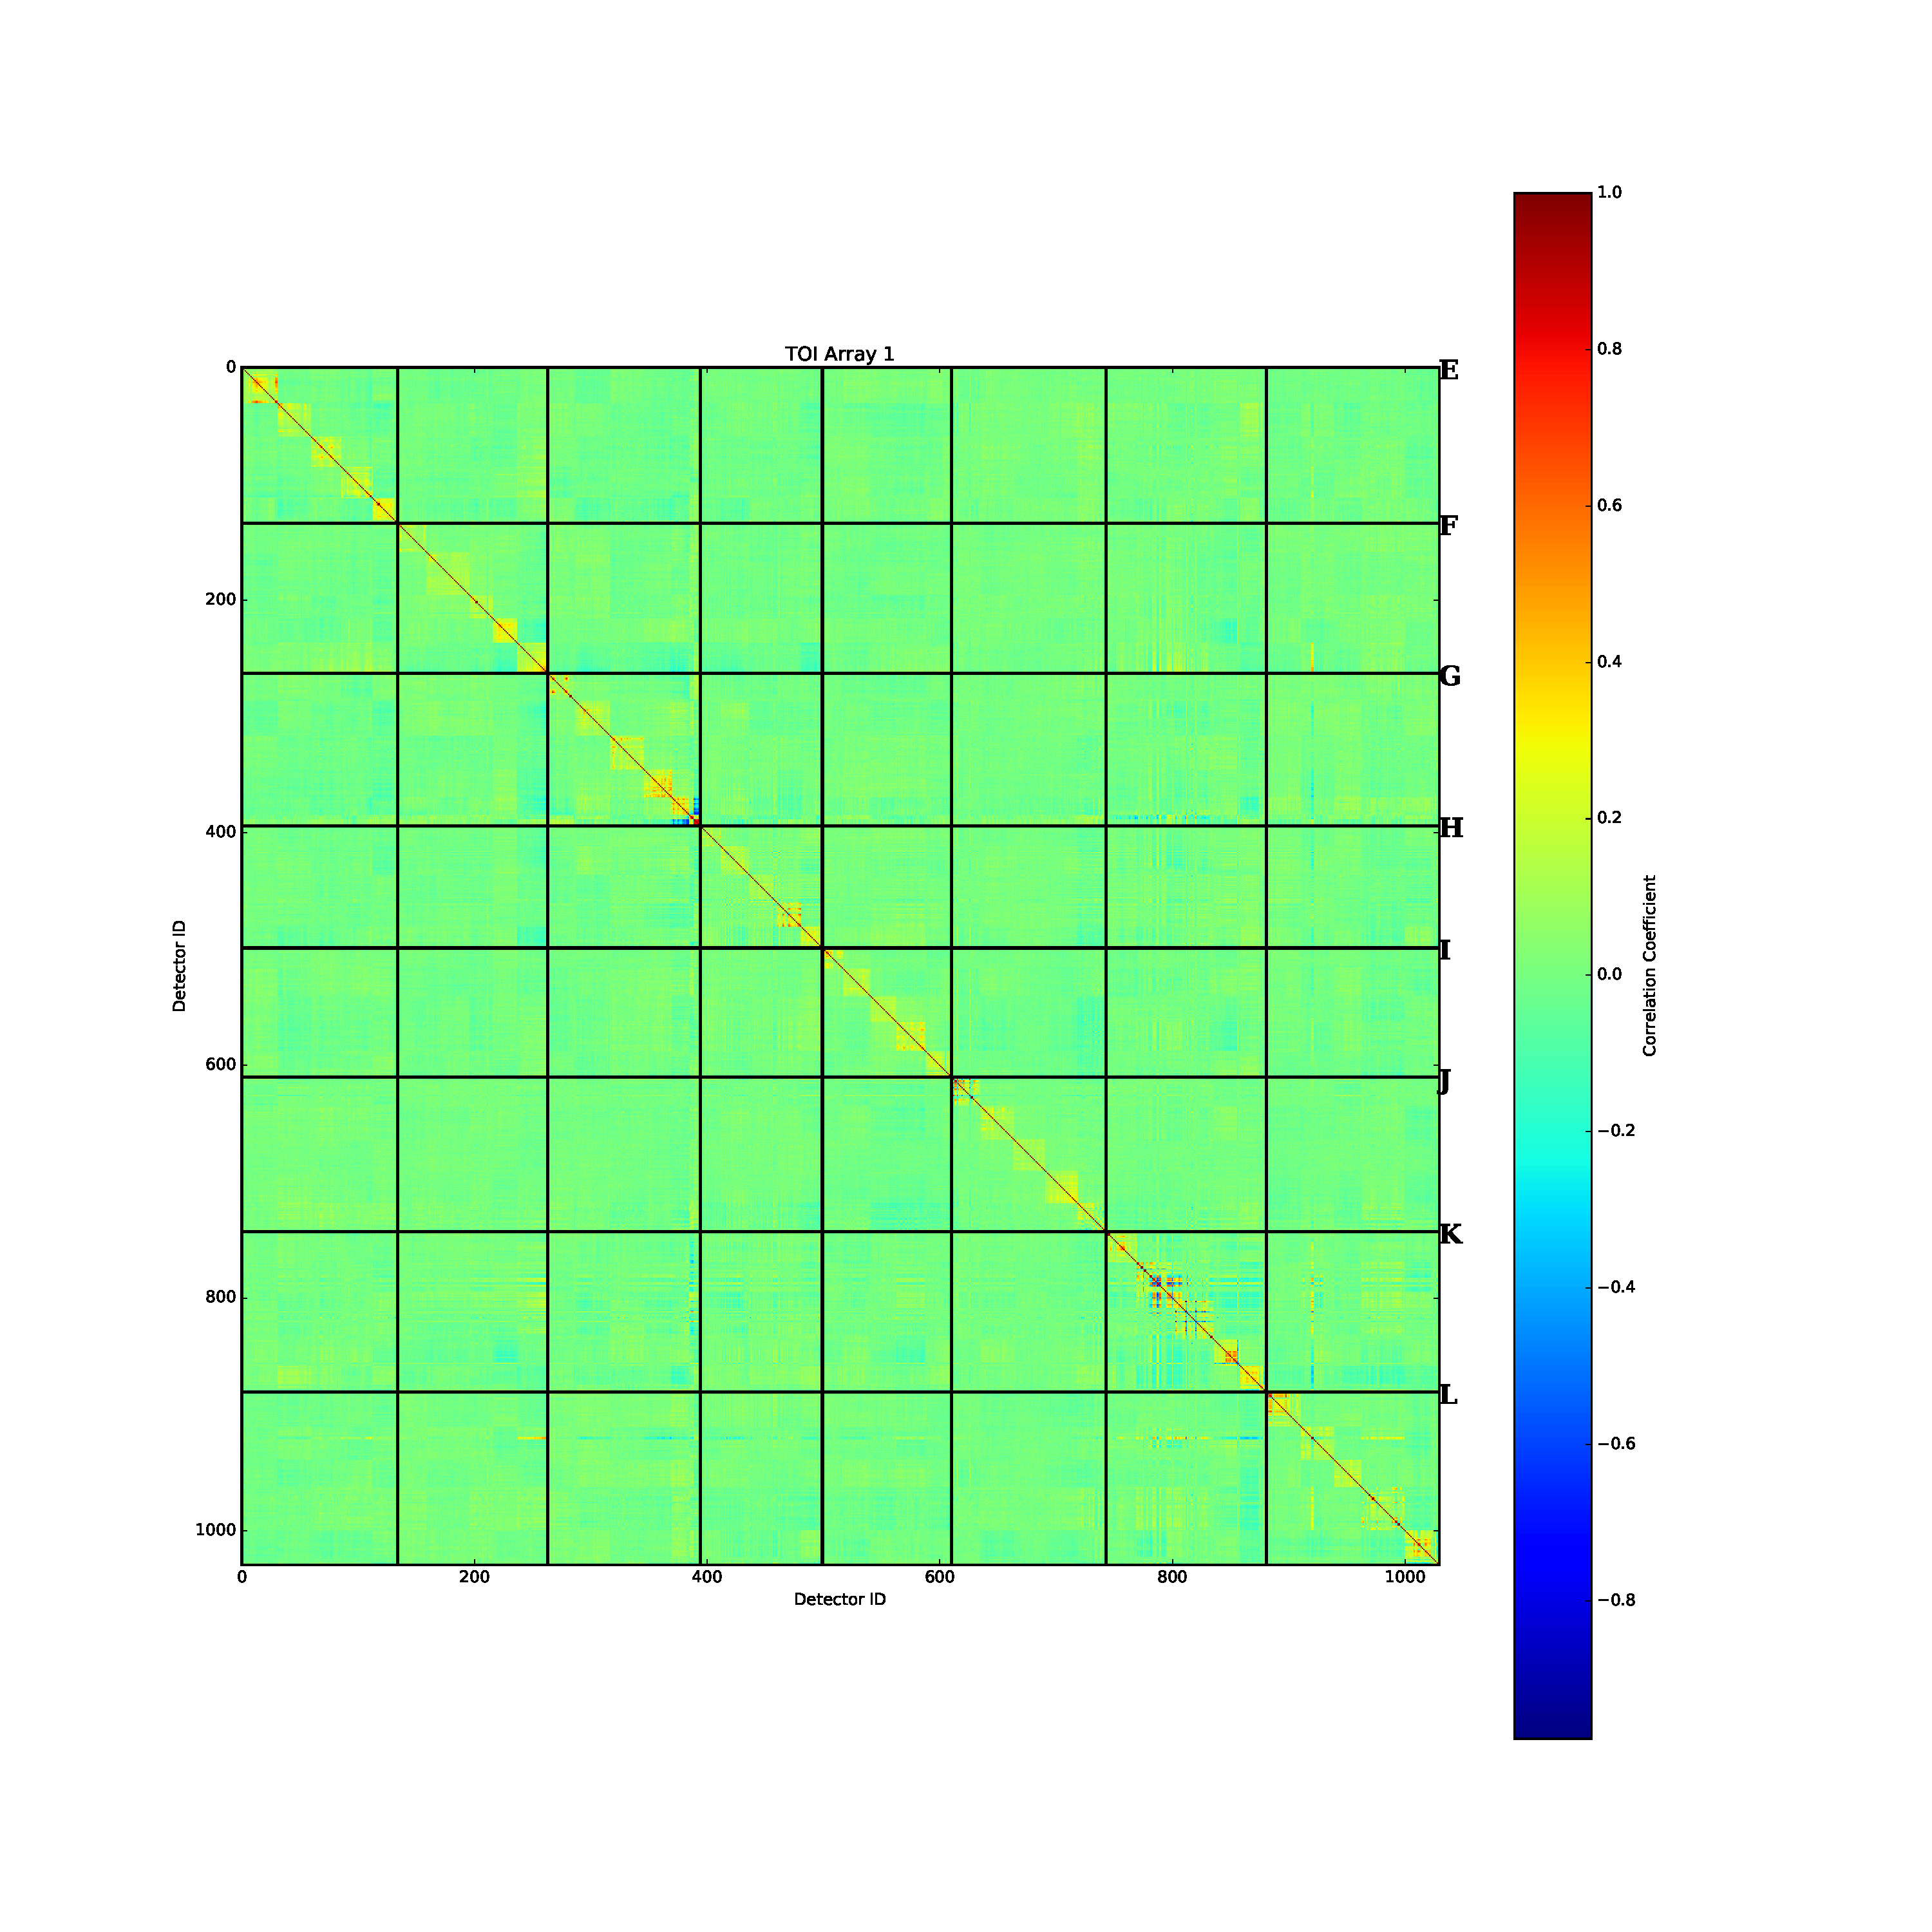
\includegraphics[width=0.3\textwidth]{Figures/DarkTests/corrmat_TOI_PCA_array_1_20161211s299.pdf}
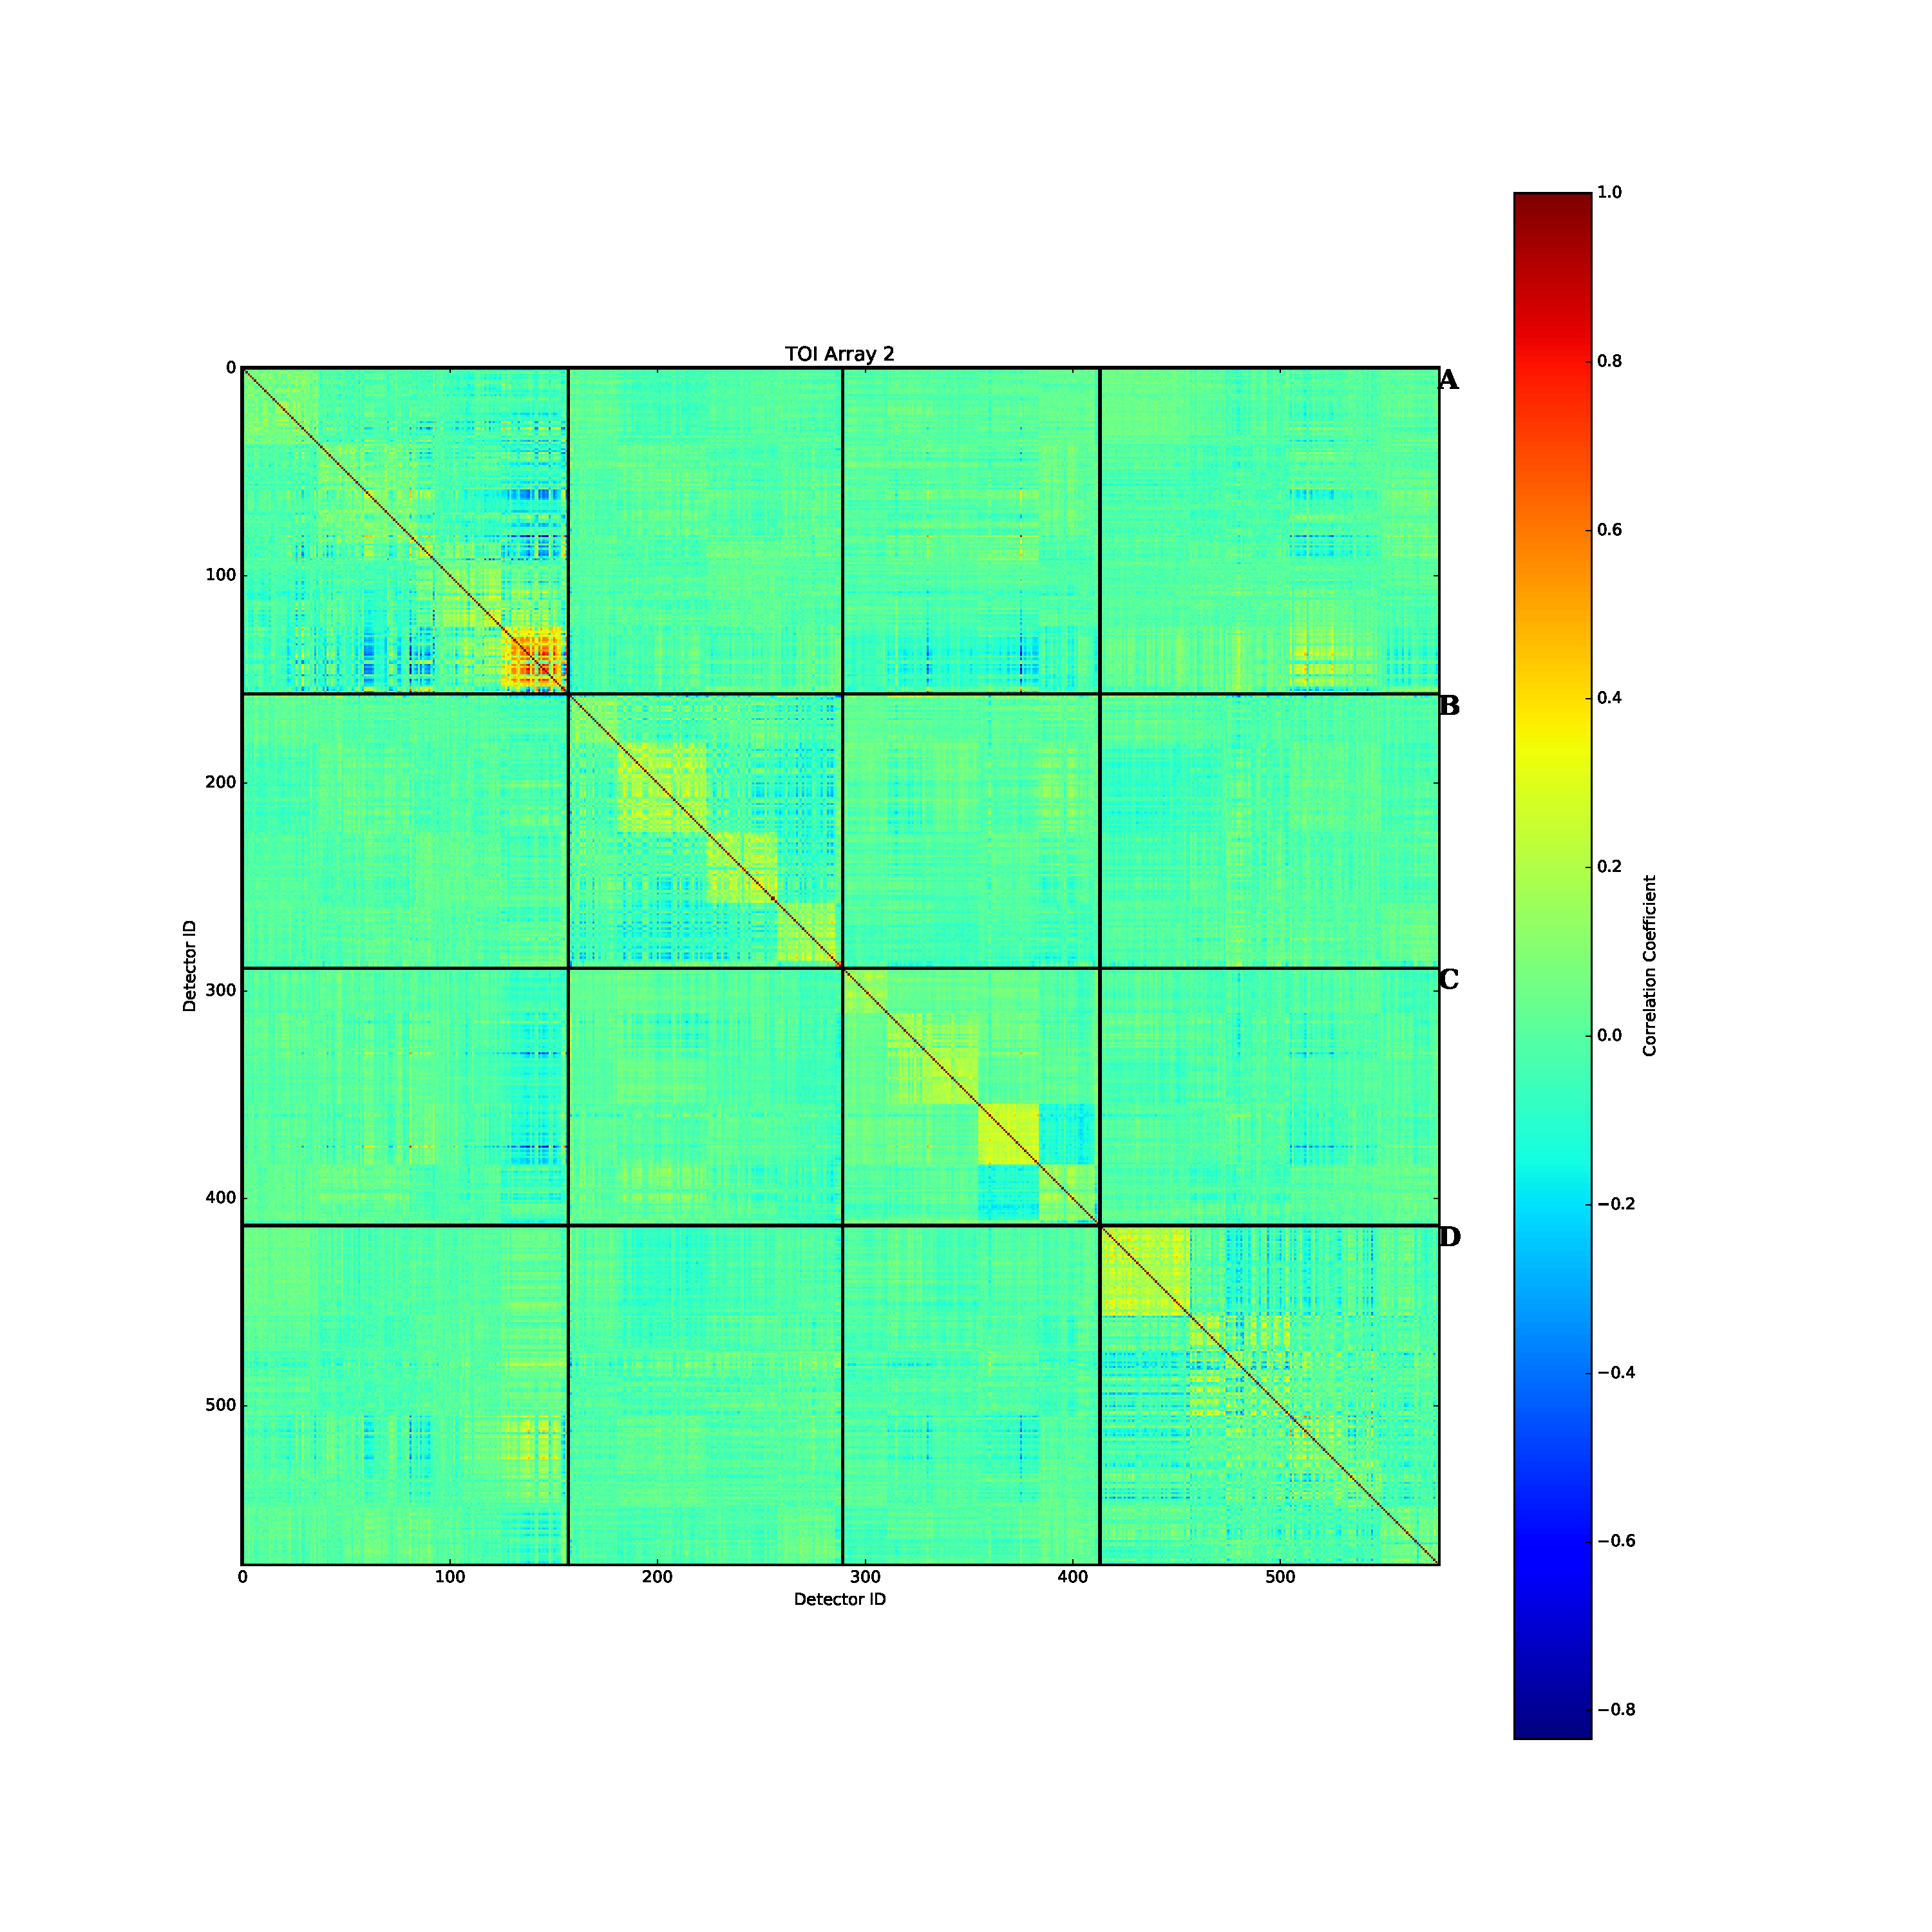
\includegraphics[width=0.3\textwidth]{Figures/DarkTests/corrmat_TOI_PCA_array_2_20161211s299.pdf}
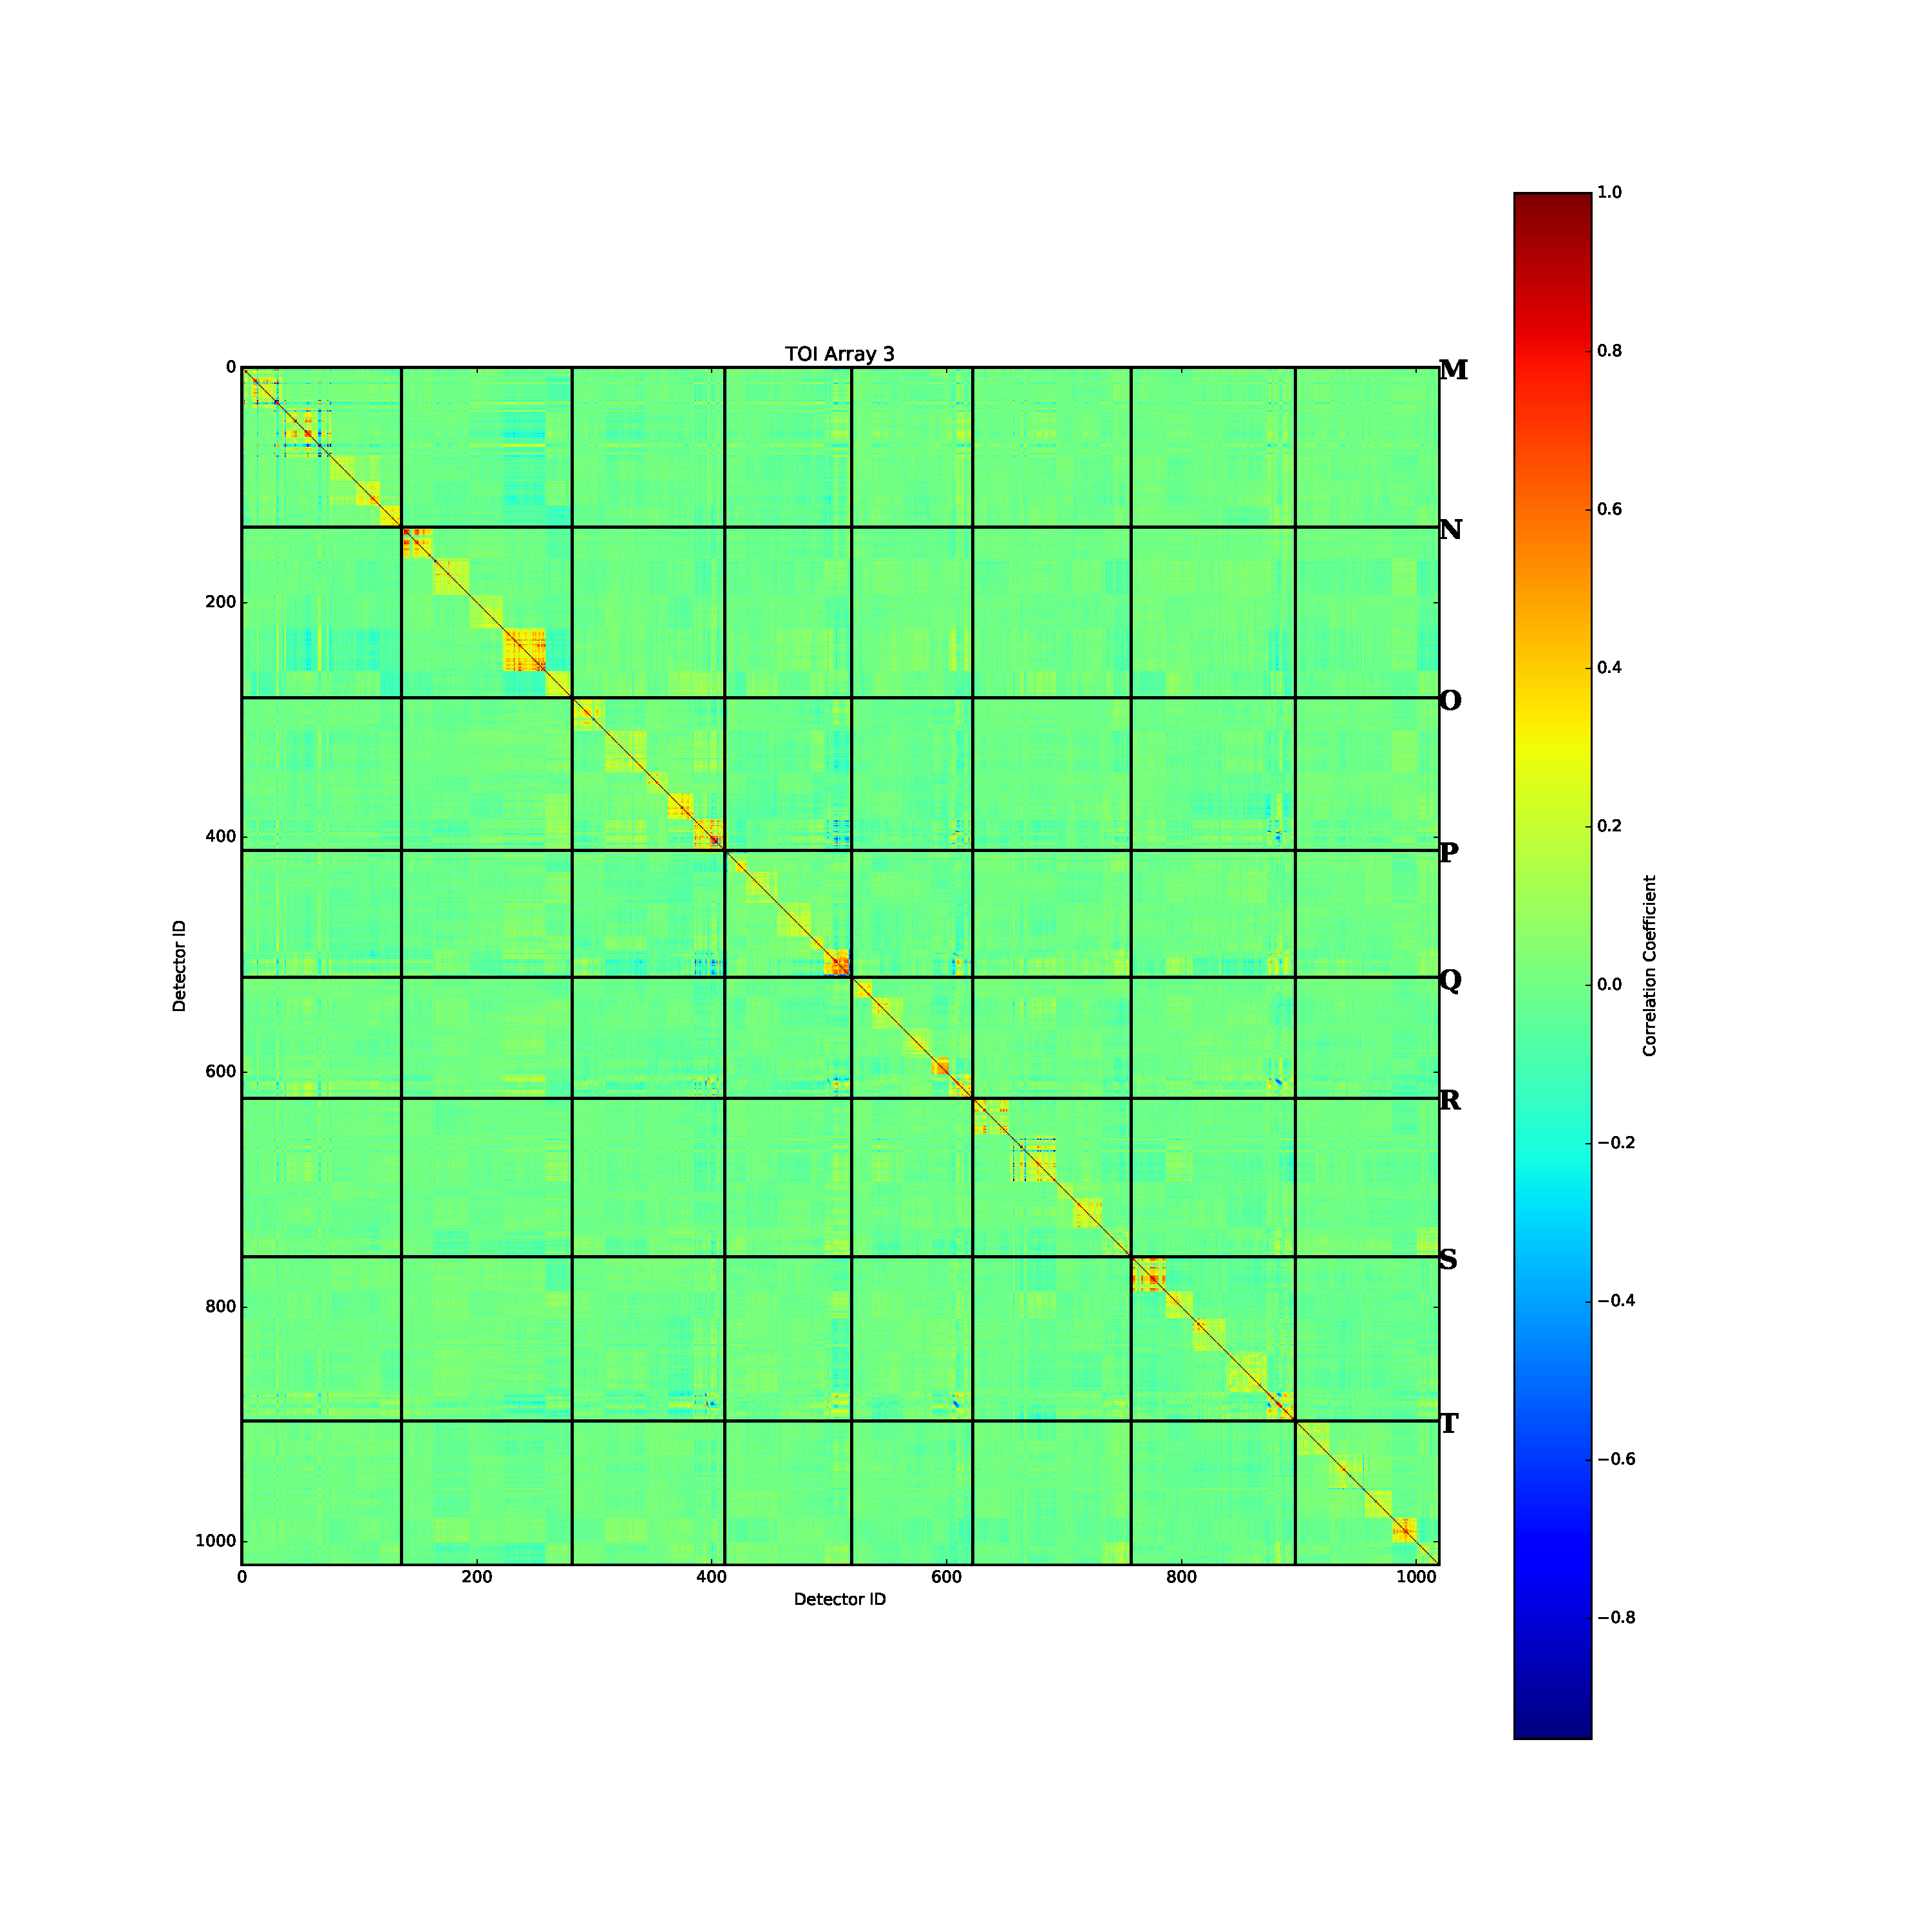
\includegraphics[width=0.3\textwidth]{Figures/DarkTests/corrmat_TOI_PCA_array_3_20161211s299.pdf}
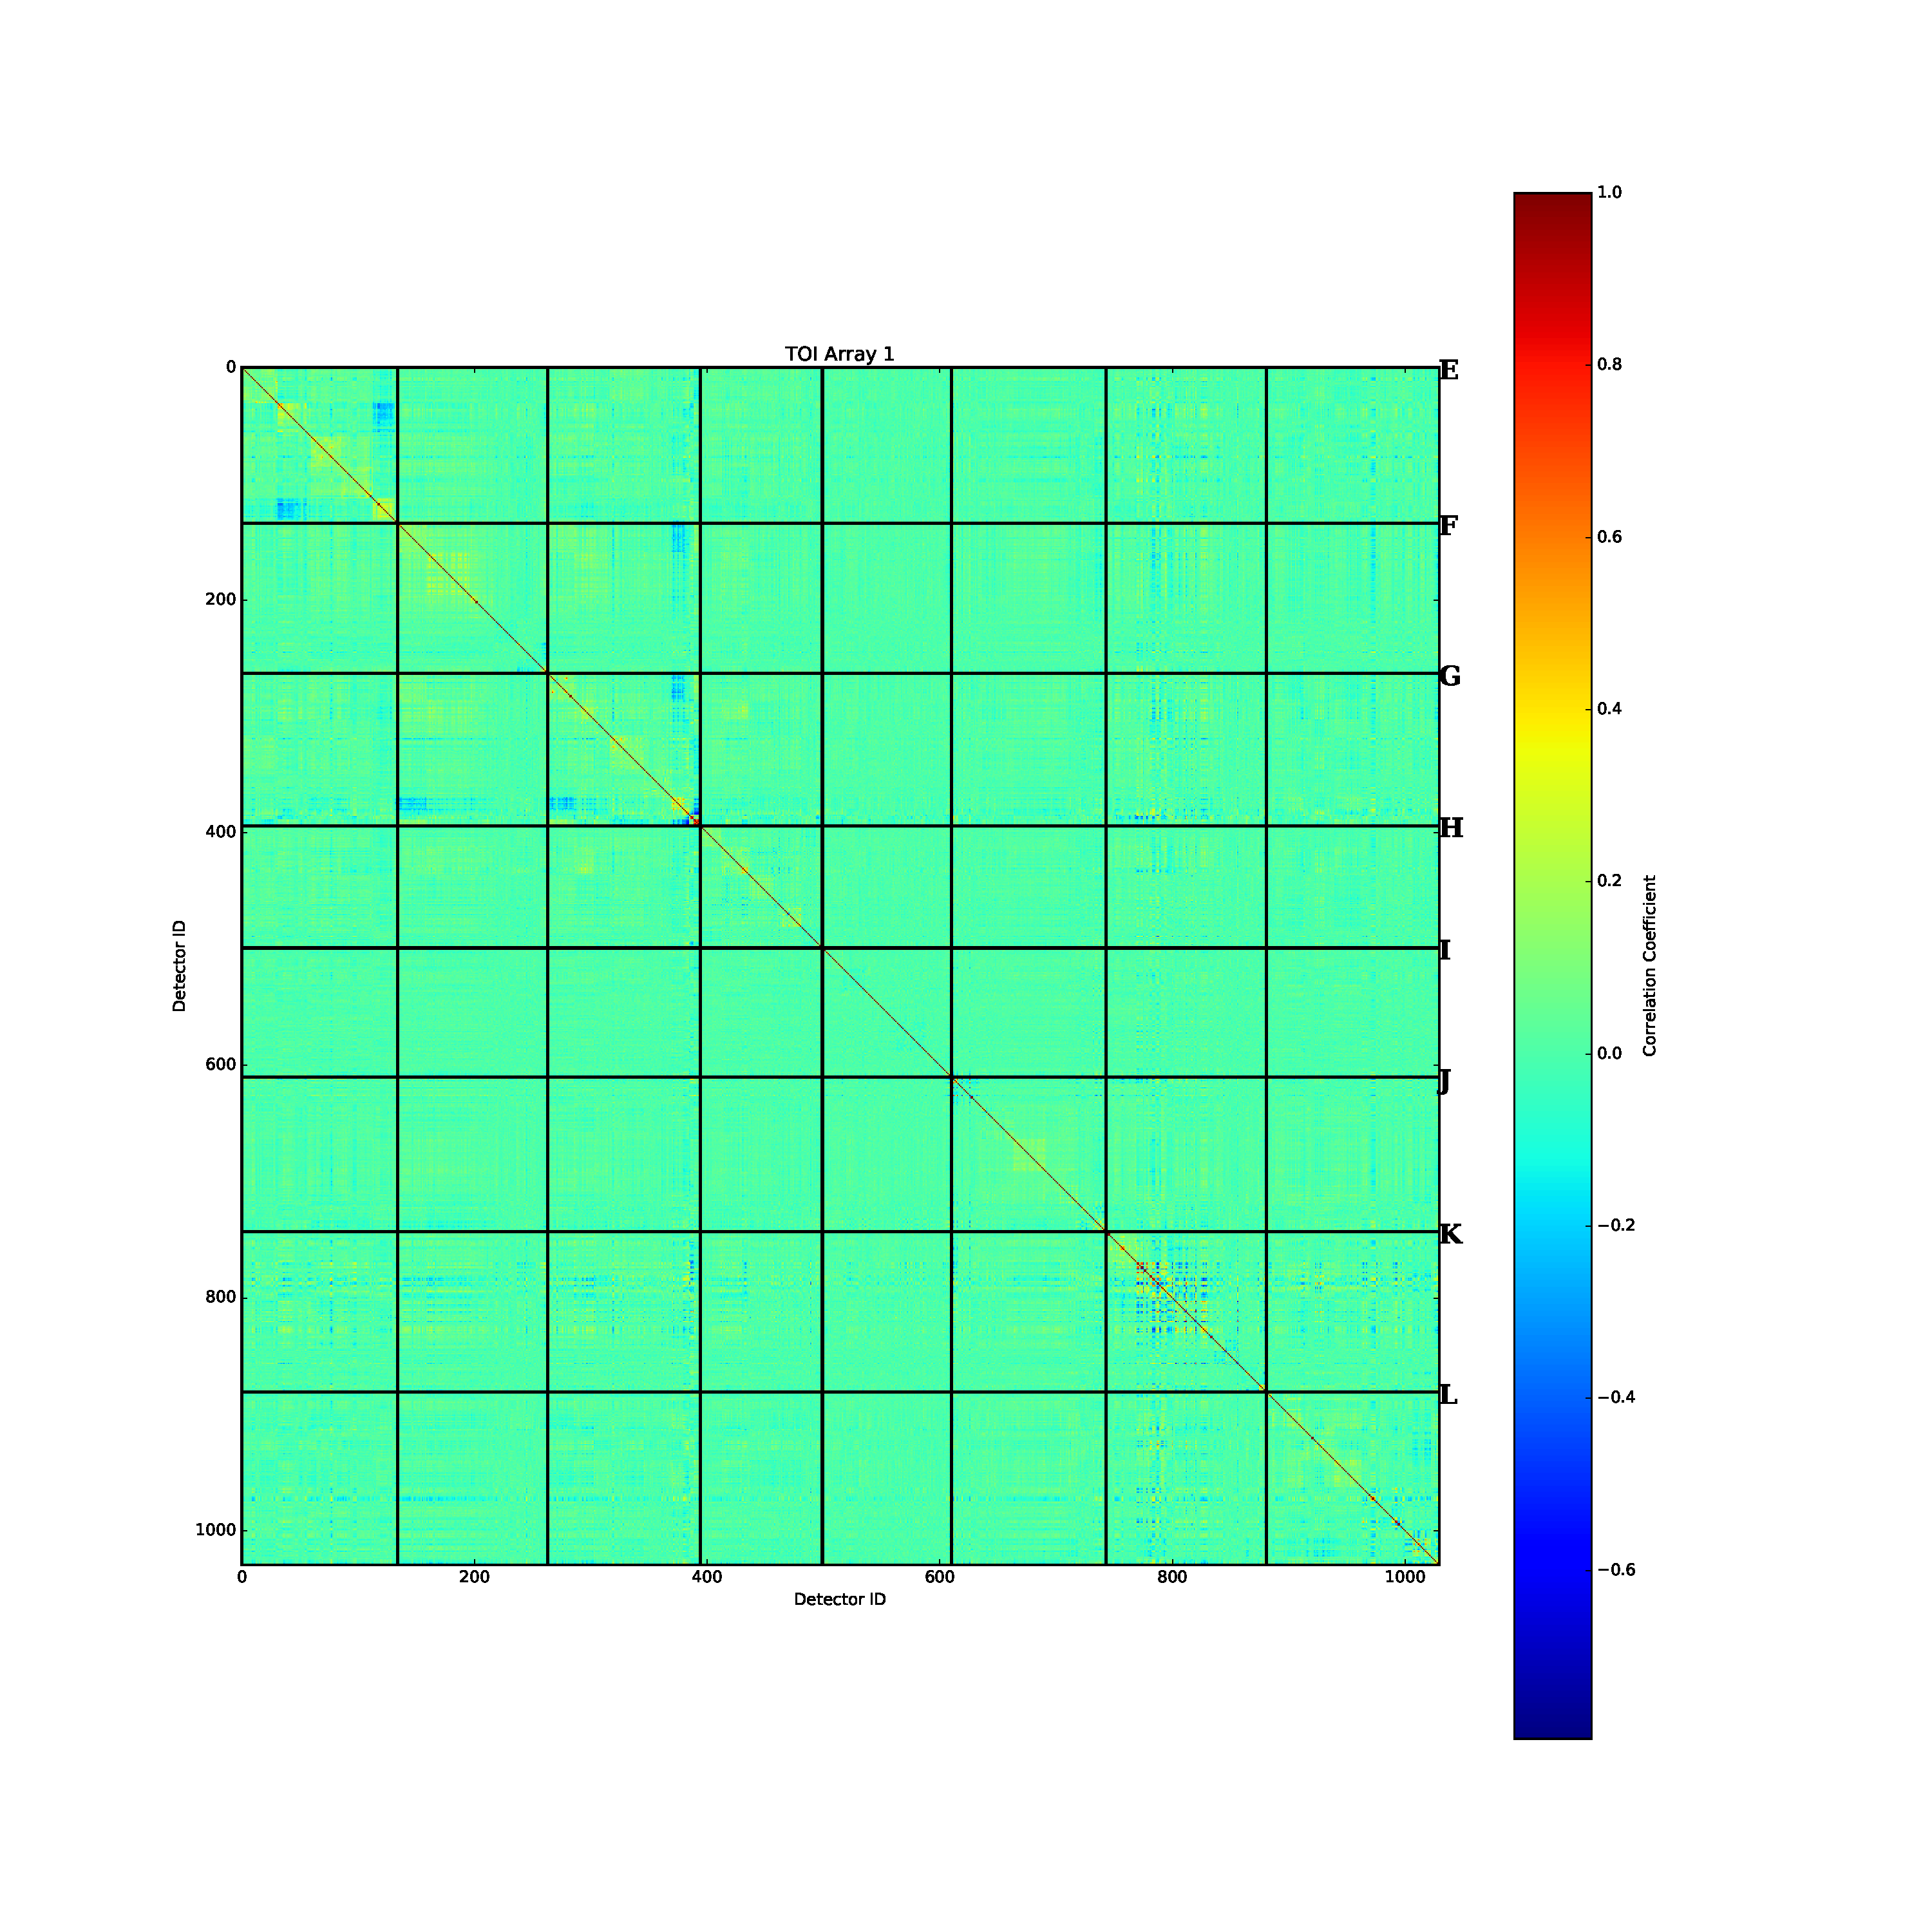
\includegraphics[width=0.3\textwidth]{Figures/DarkTests/corrmat_TOI_BC_array_1_20161211s299.pdf}
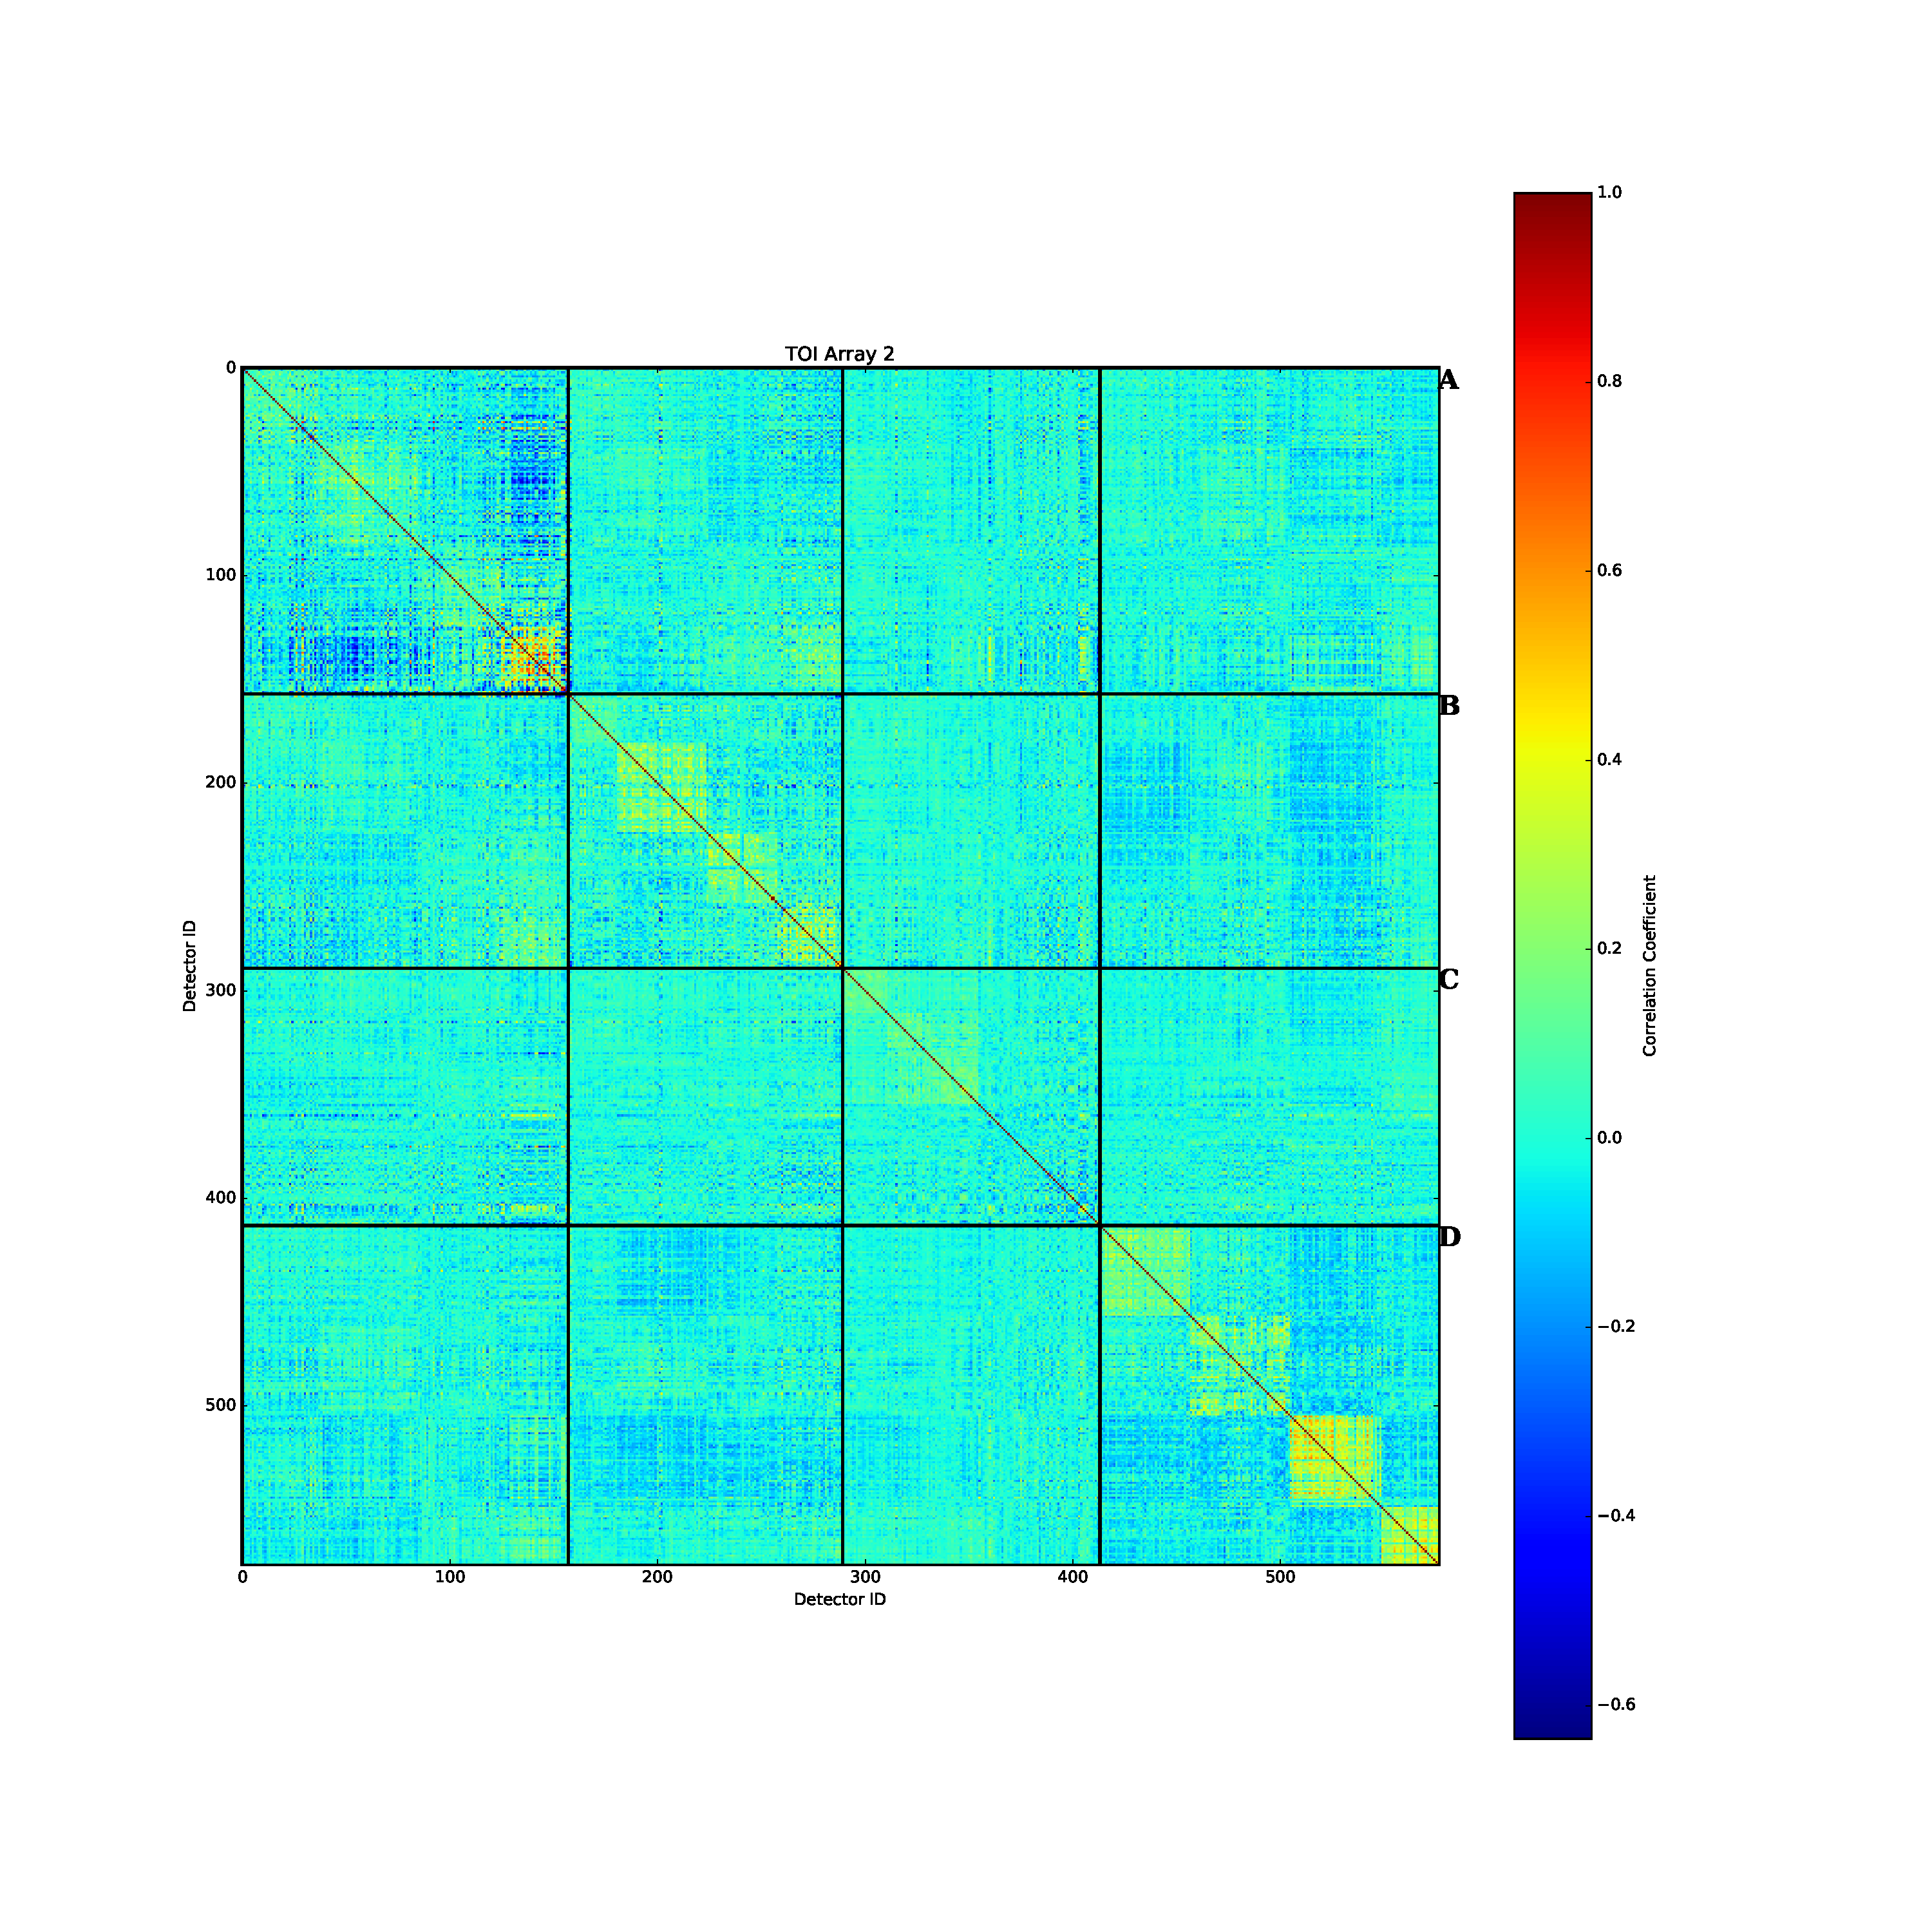
\includegraphics[width=0.3\textwidth]{Figures/DarkTests/corrmat_TOI_BC_array_2_20161211s299.pdf}
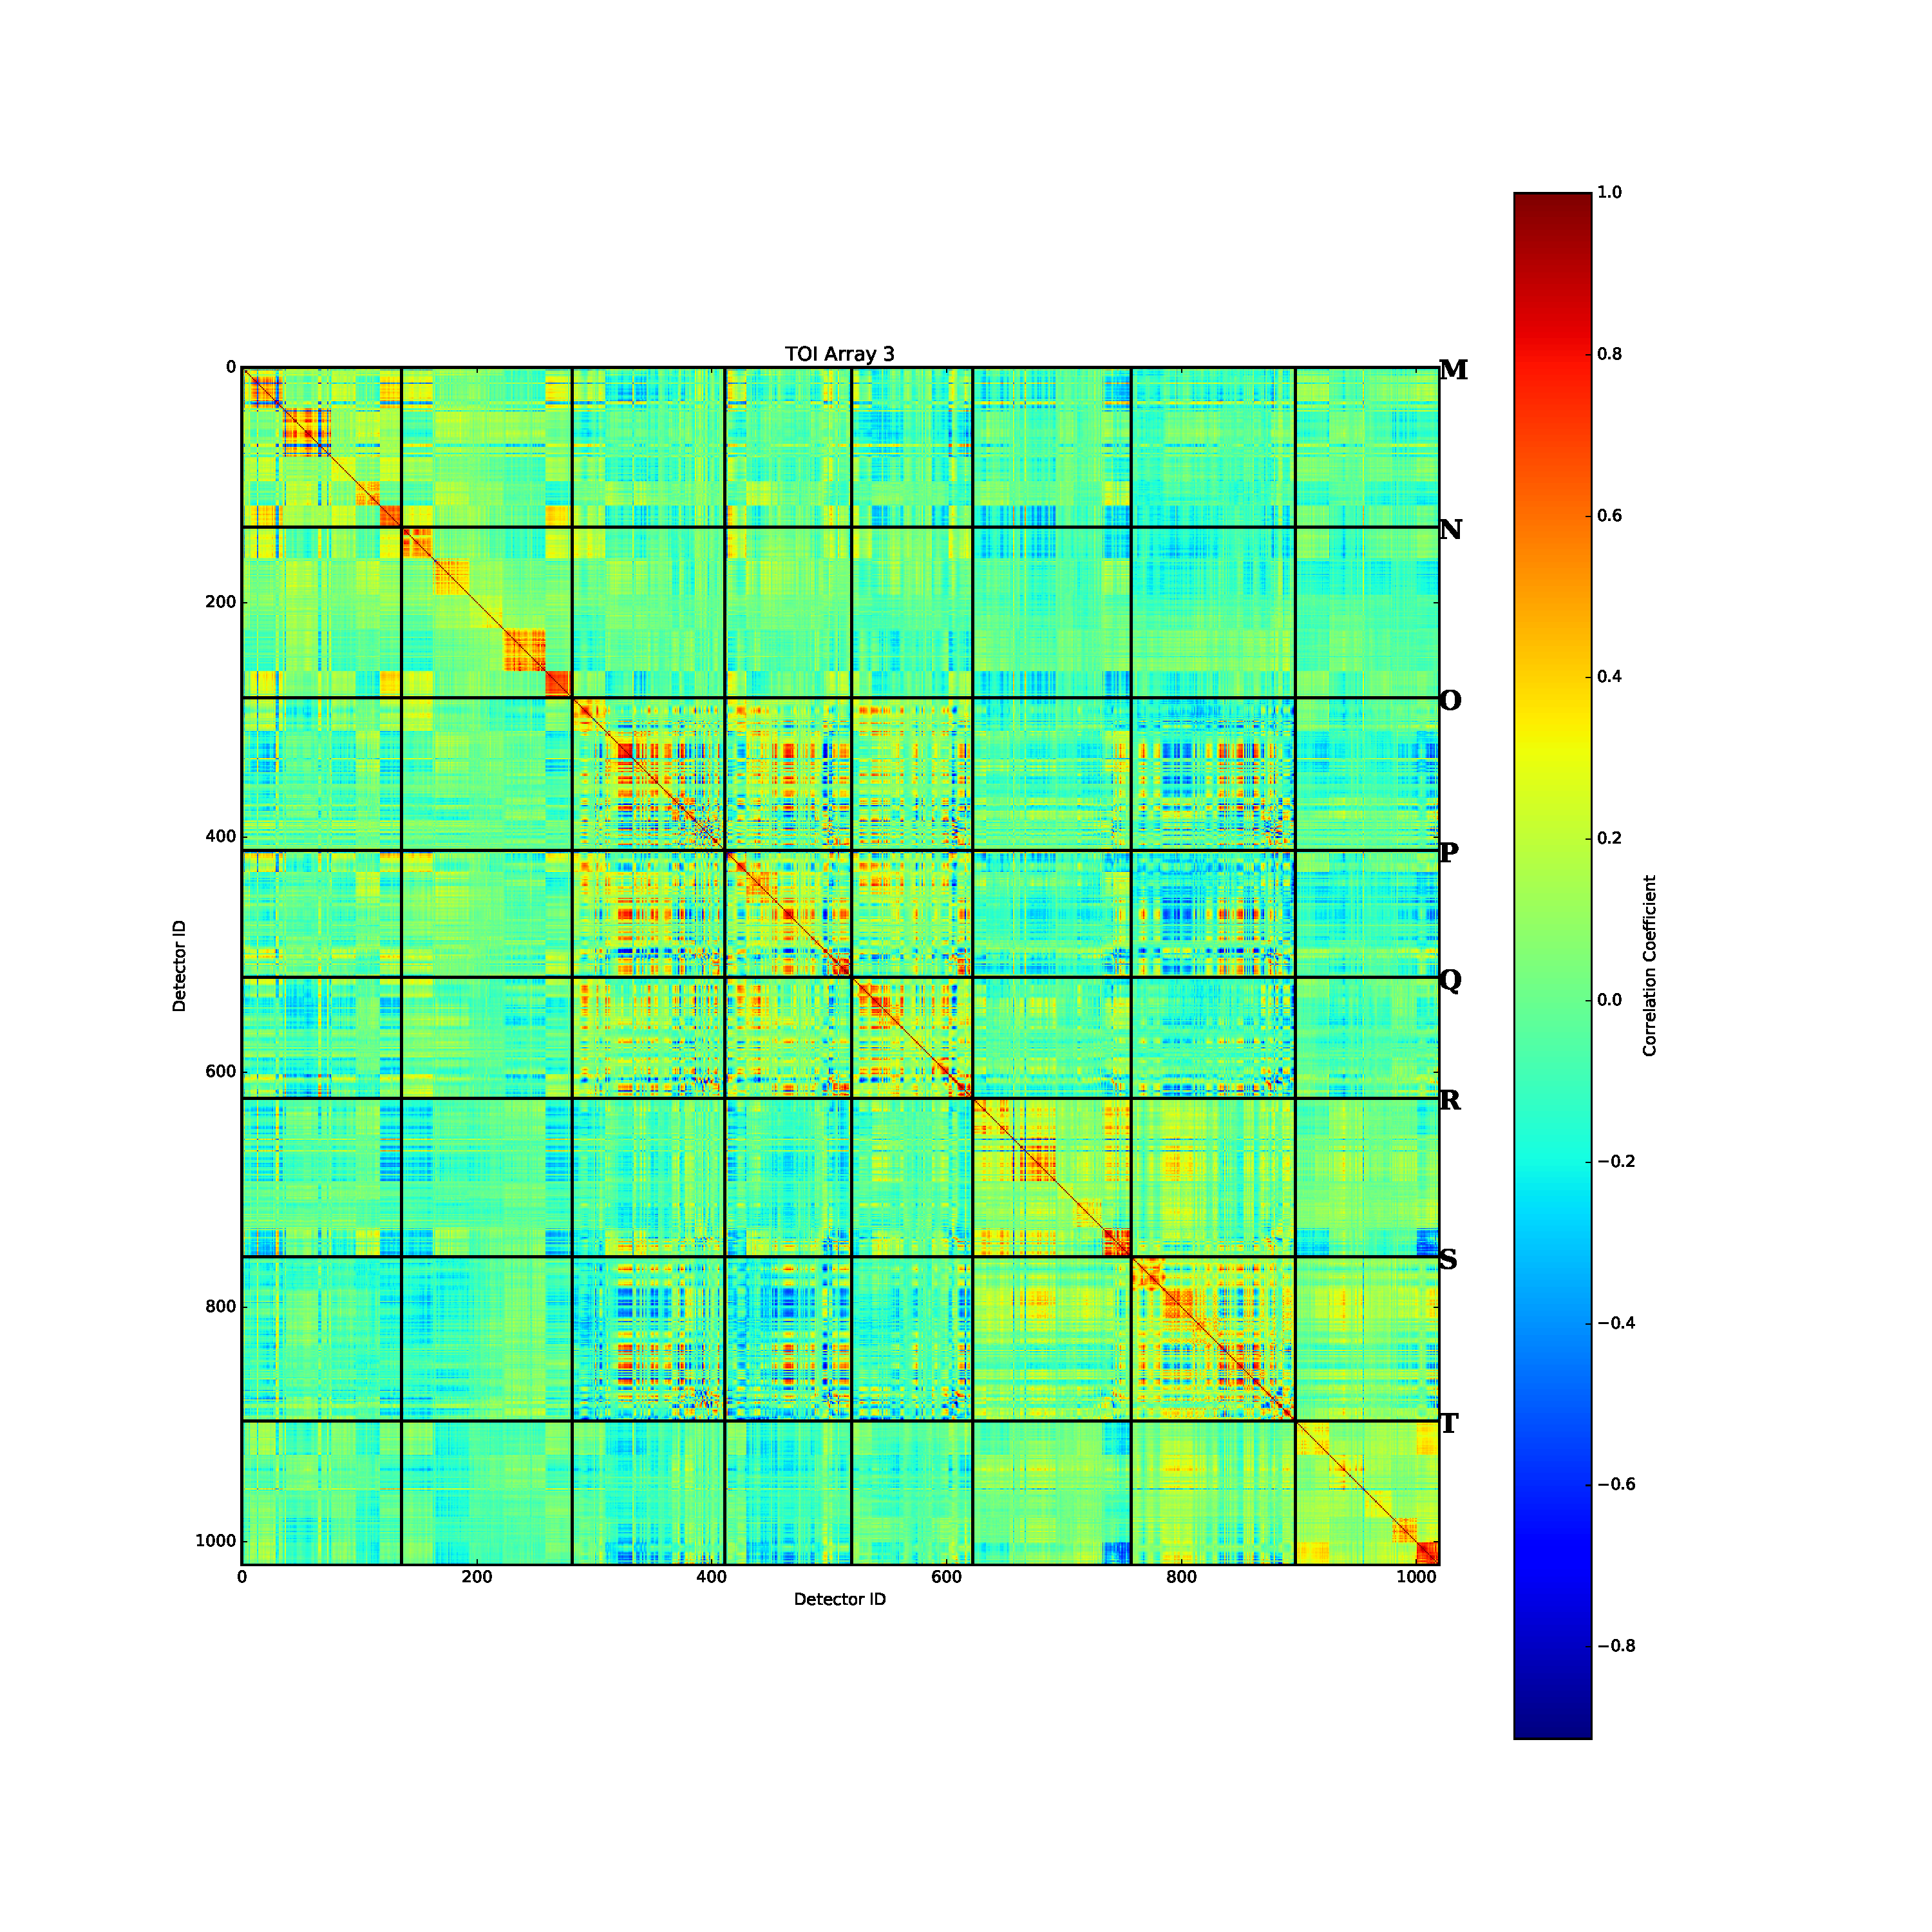
\includegraphics[width=0.3\textwidth]{Figures/DarkTests/corrmat_TOI_BC_array_3_20161211s299.pdf}
\end{center}
\caption{From left to right correlation matrices for the three NIKA2 arrays (A1, A2, and A3) for scan 20161211s299. From top to bottom we present the correlation of the raw data, after CM, PCA and BC decorrelations. \label{corrs299}}
\end{figure}



\begin{figure}[ht] % Inline image example
\begin{center}
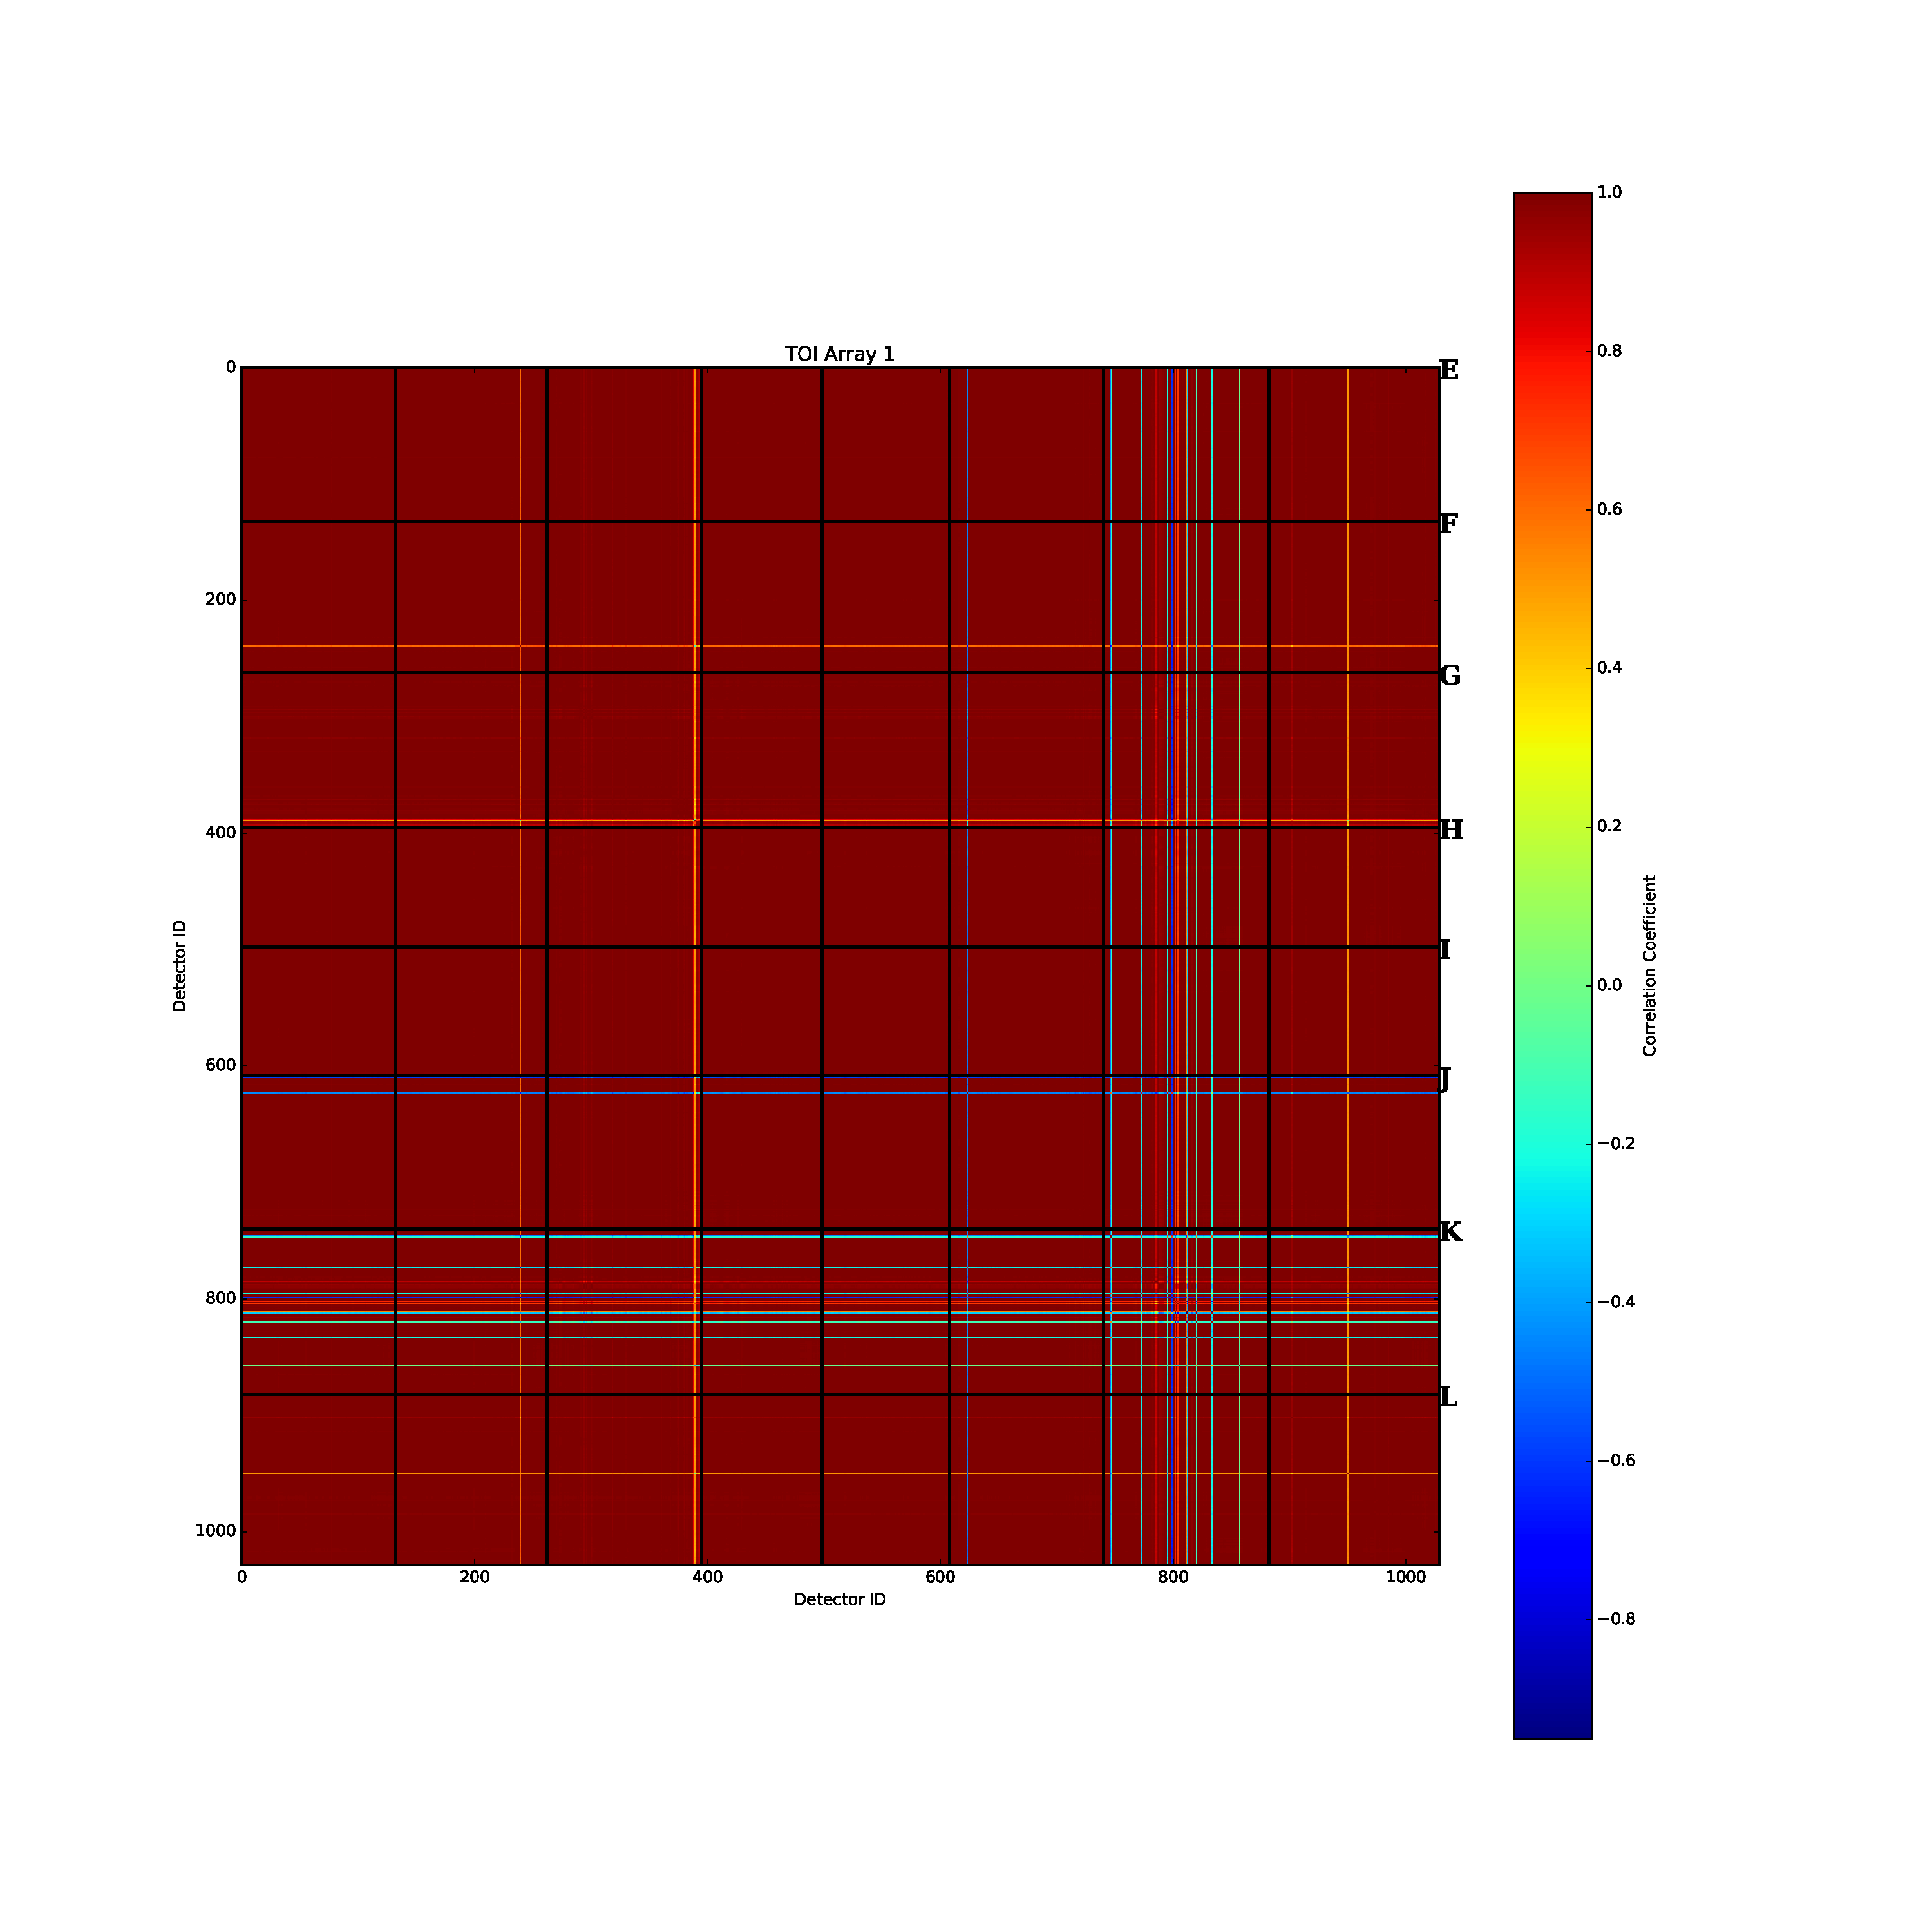
\includegraphics[width=0.3\textwidth]{Figures/DarkTests/corrmat_TOI_array_1_20161213s72.pdf}
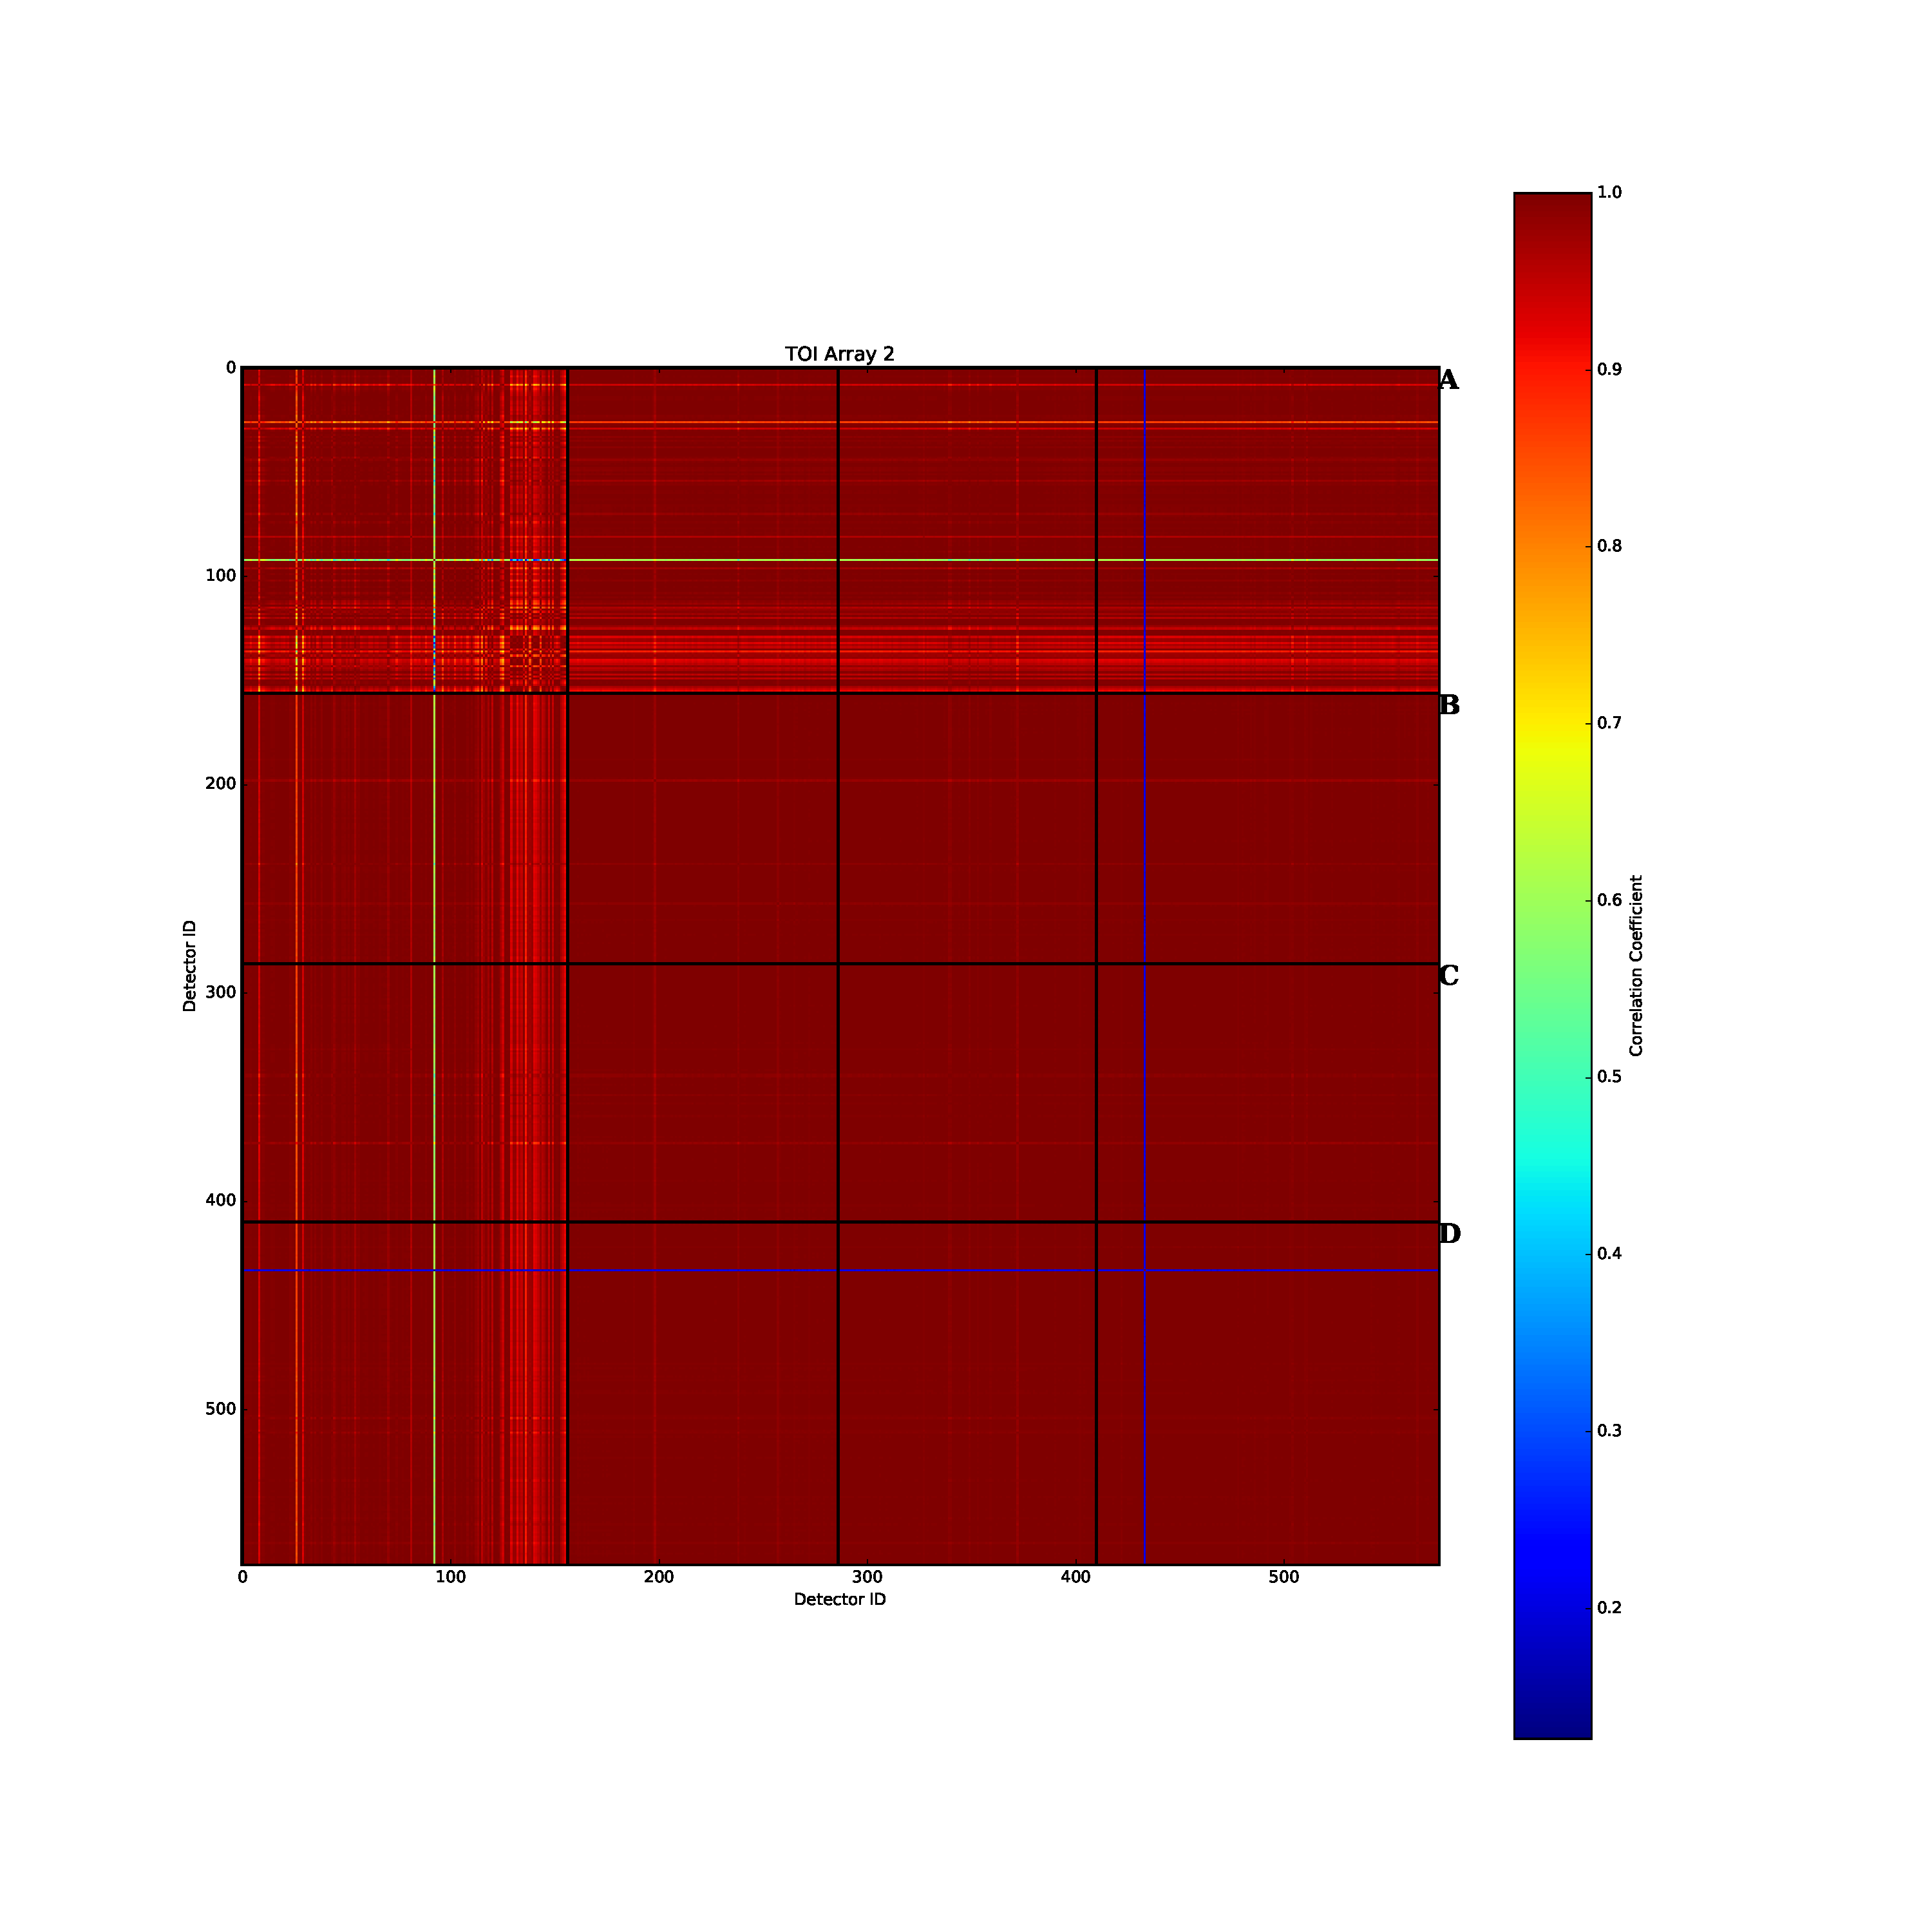
\includegraphics[width=0.3\textwidth]{Figures/DarkTests/corrmat_TOI_array_2_20161213s72.pdf}
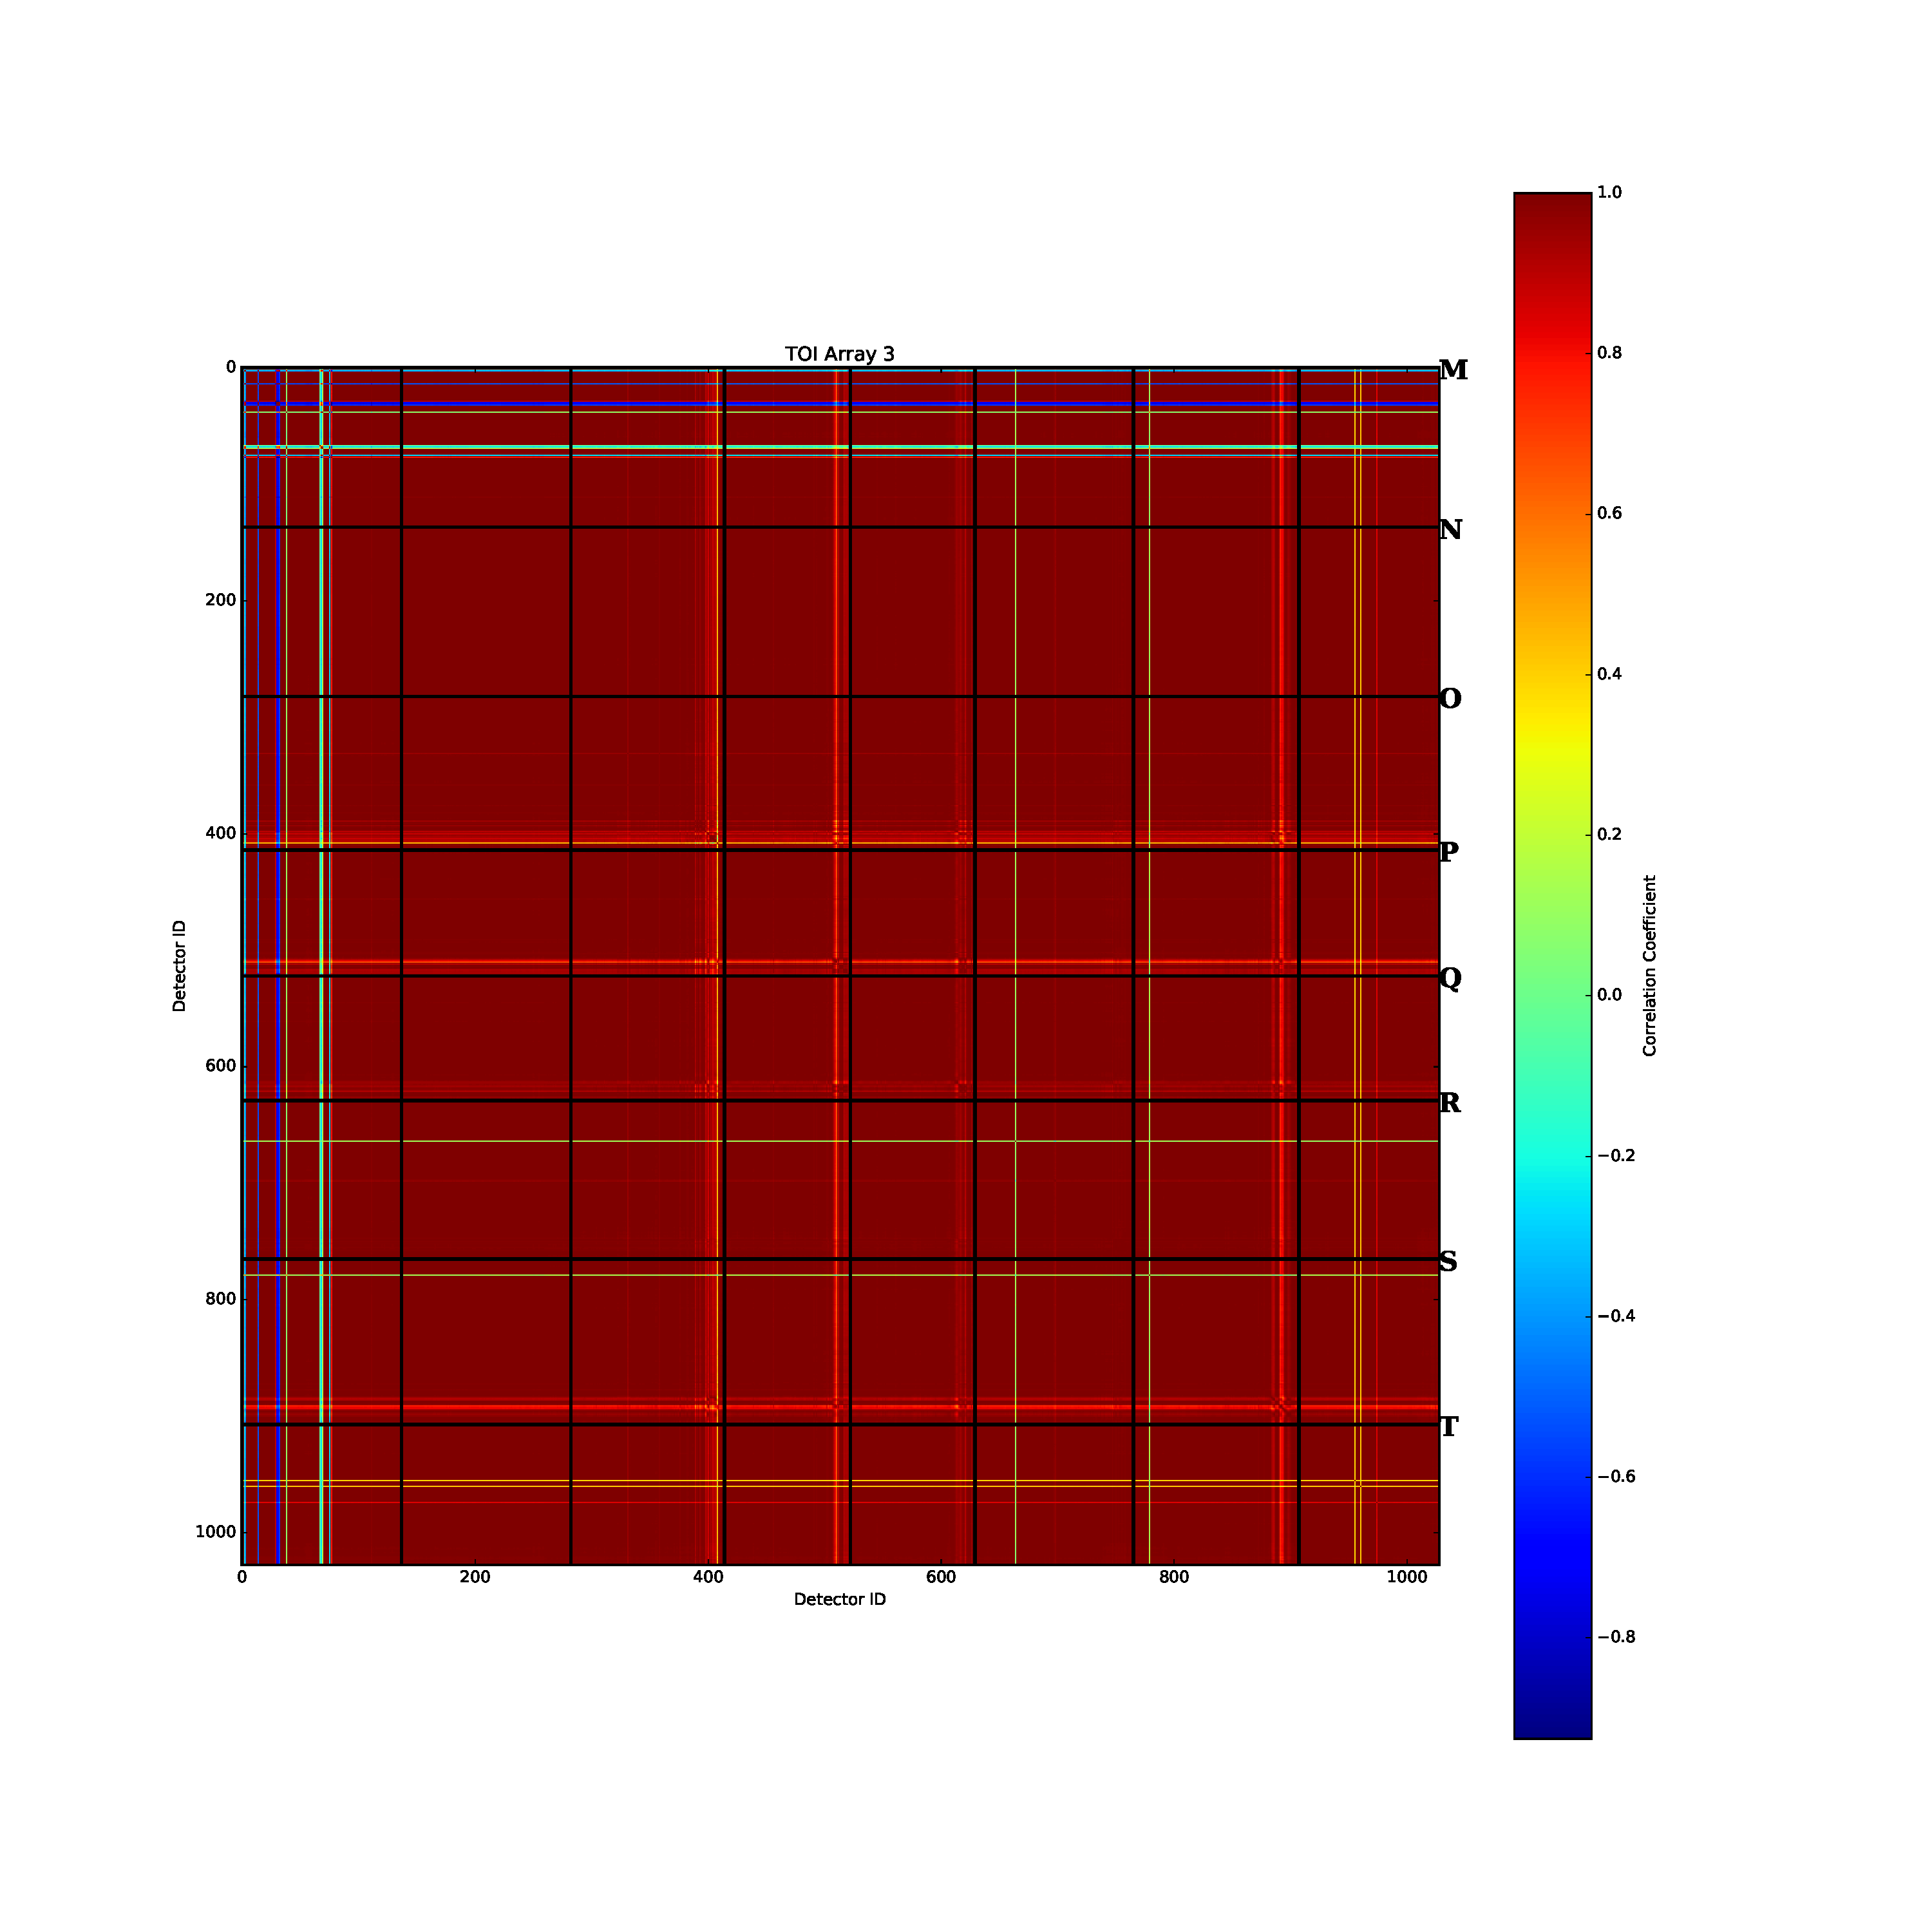
\includegraphics[width=0.3\textwidth]{Figures/DarkTests/corrmat_TOI_array_3_20161213s72.pdf}
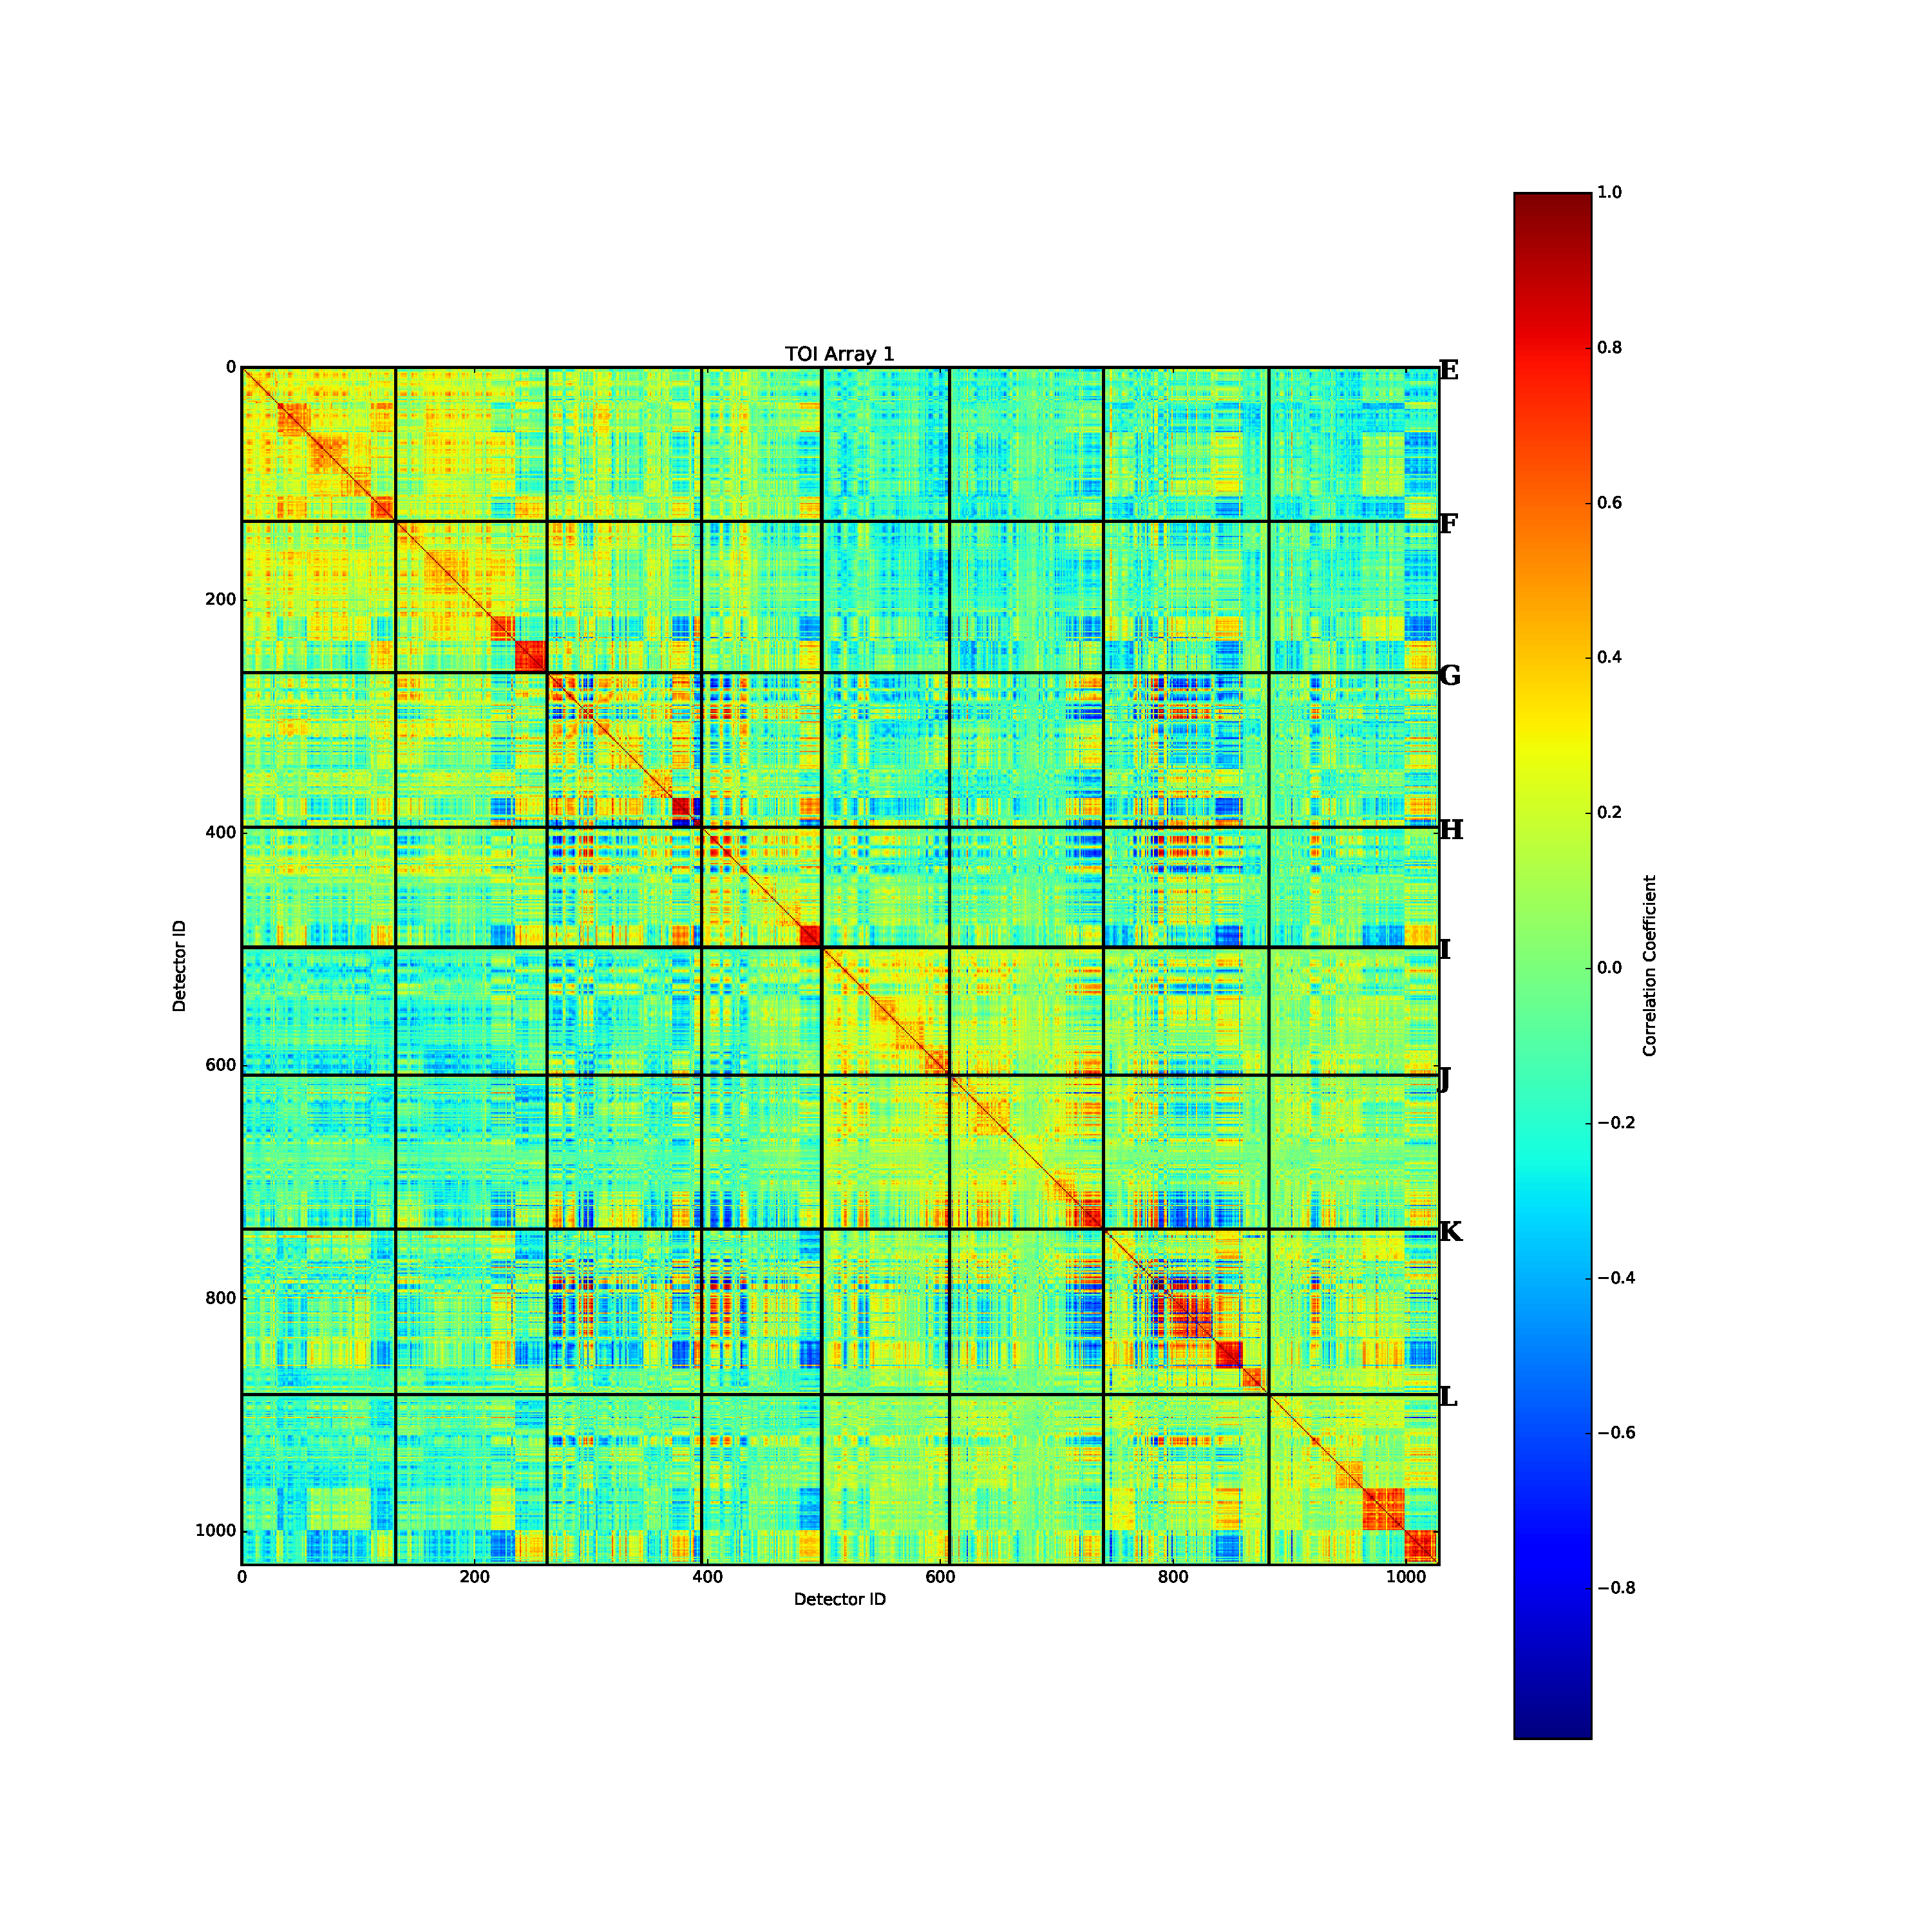
\includegraphics[width=0.3\textwidth]{Figures/DarkTests/corrmat_TOI_CM_array_1_20161213s72.pdf}
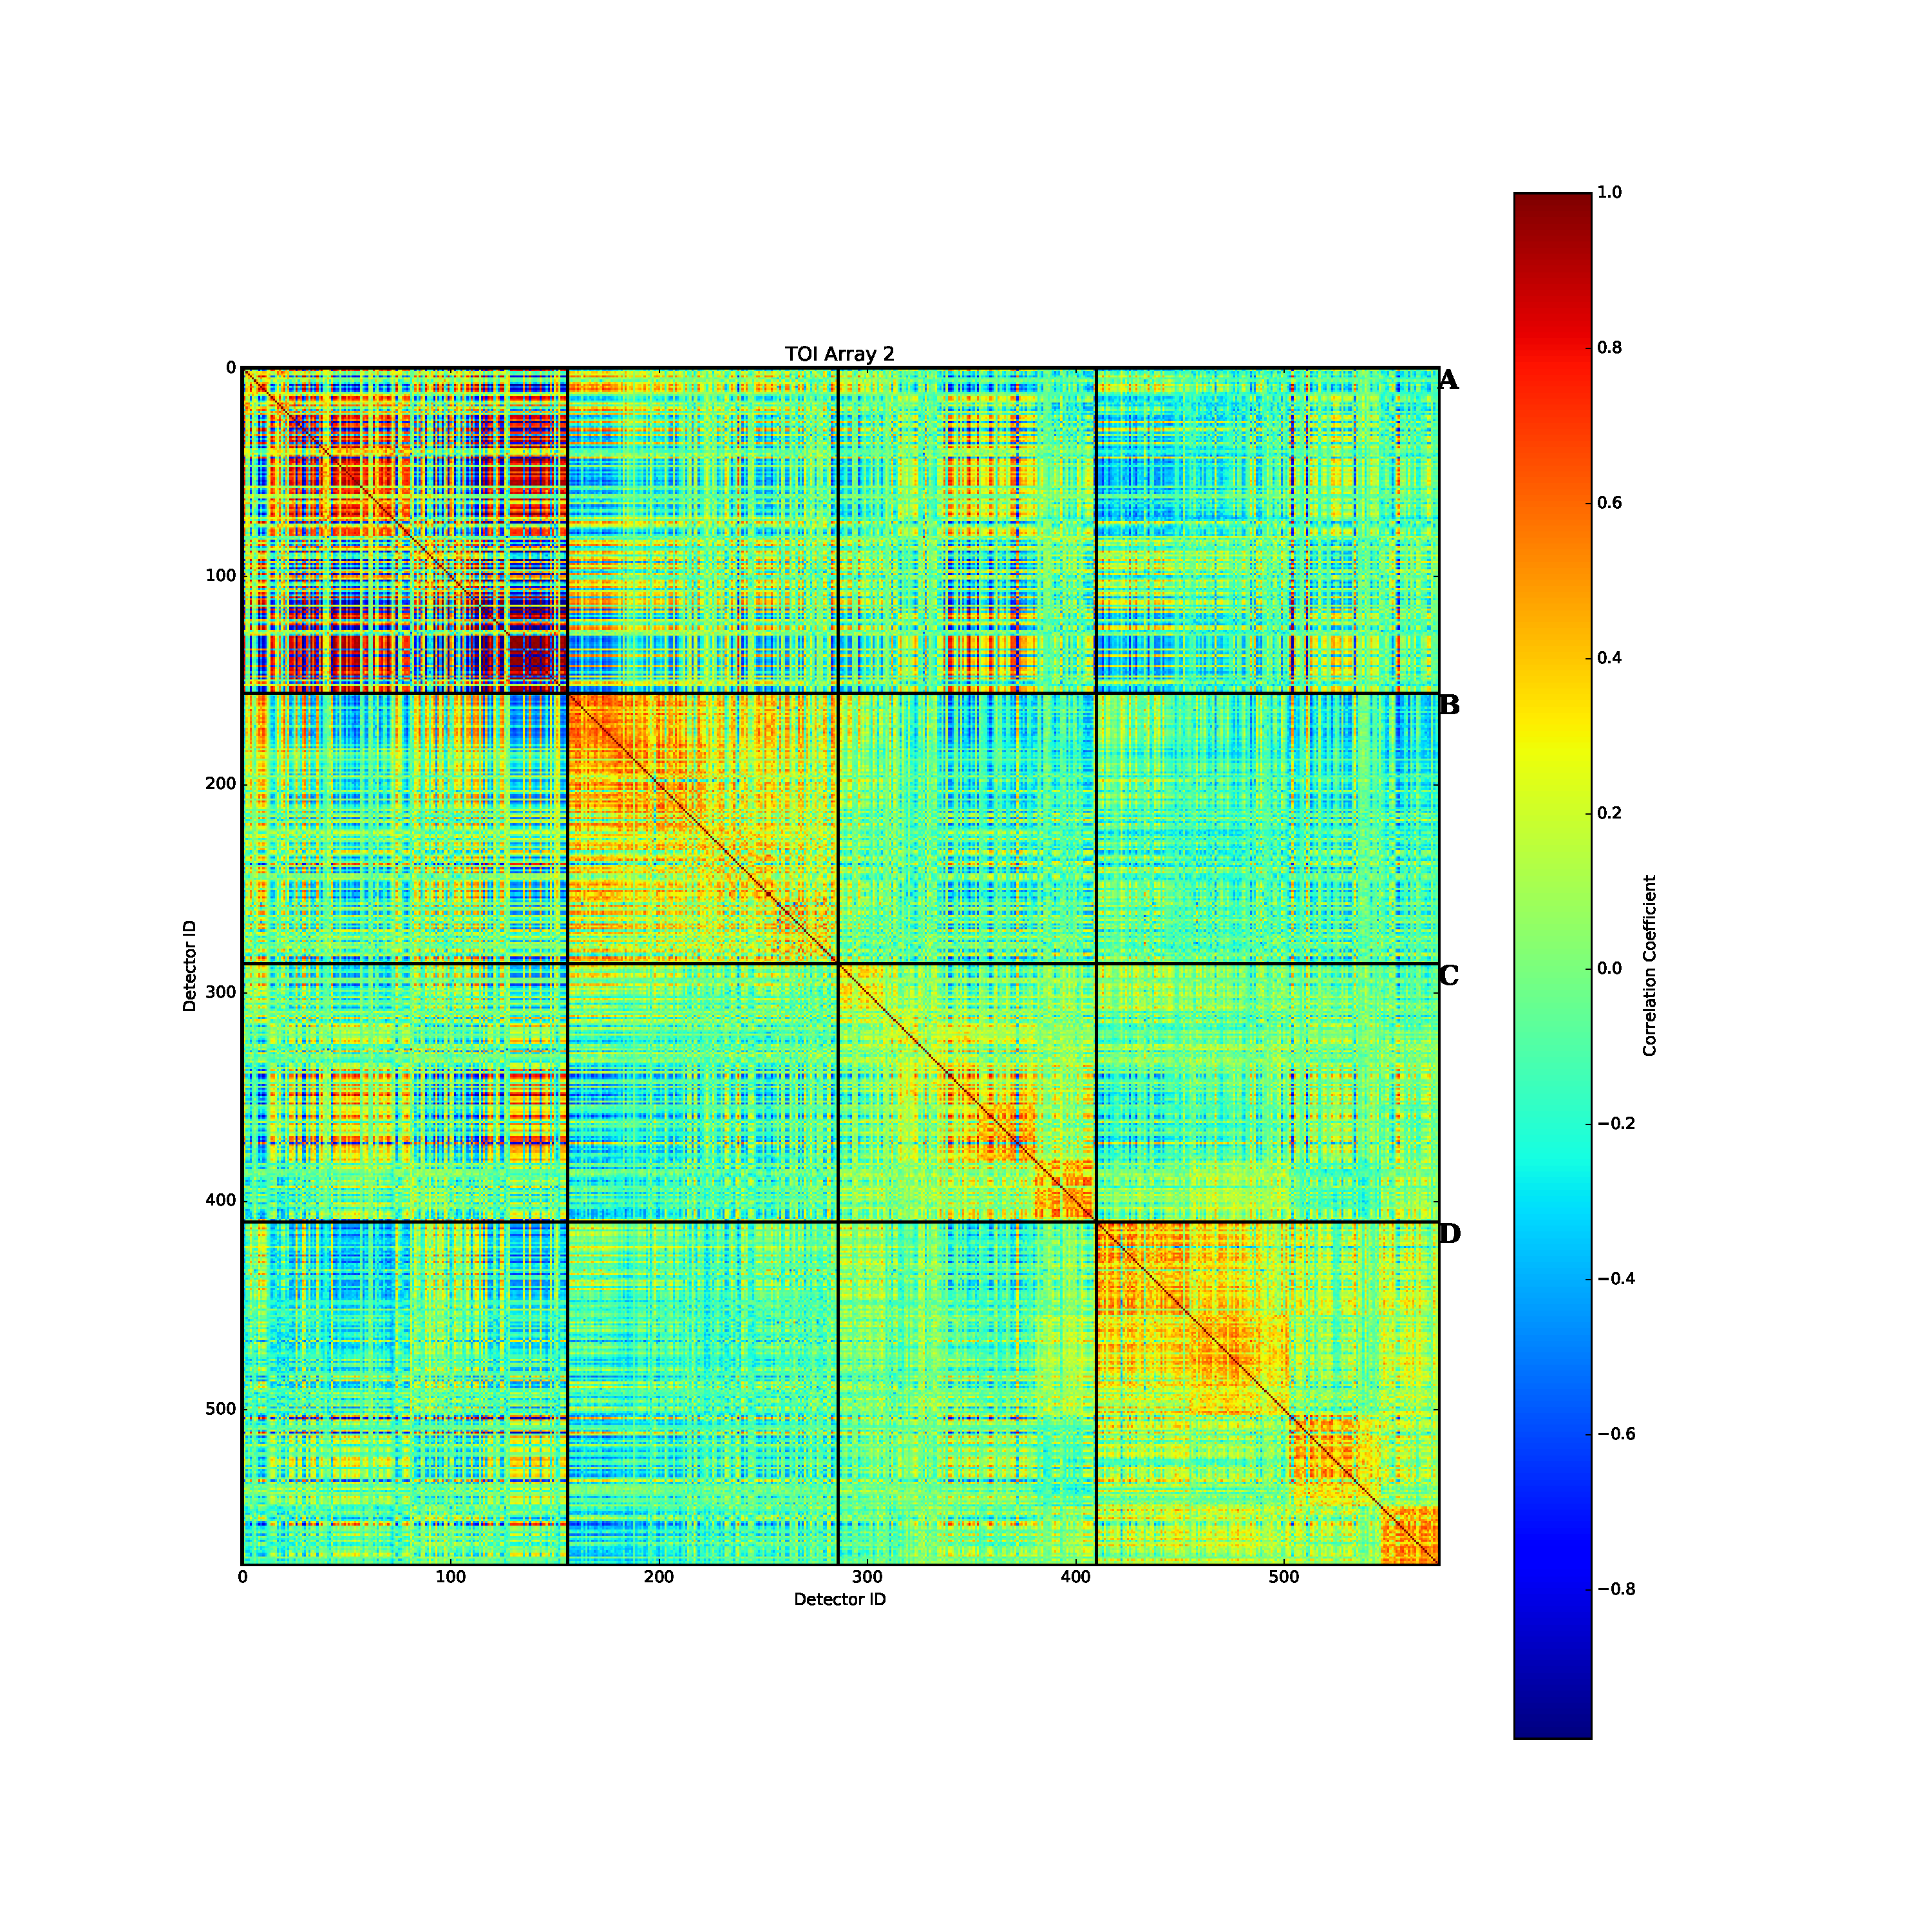
\includegraphics[width=0.3\textwidth]{Figures/DarkTests/corrmat_TOI_CM_array_2_20161213s72.pdf}
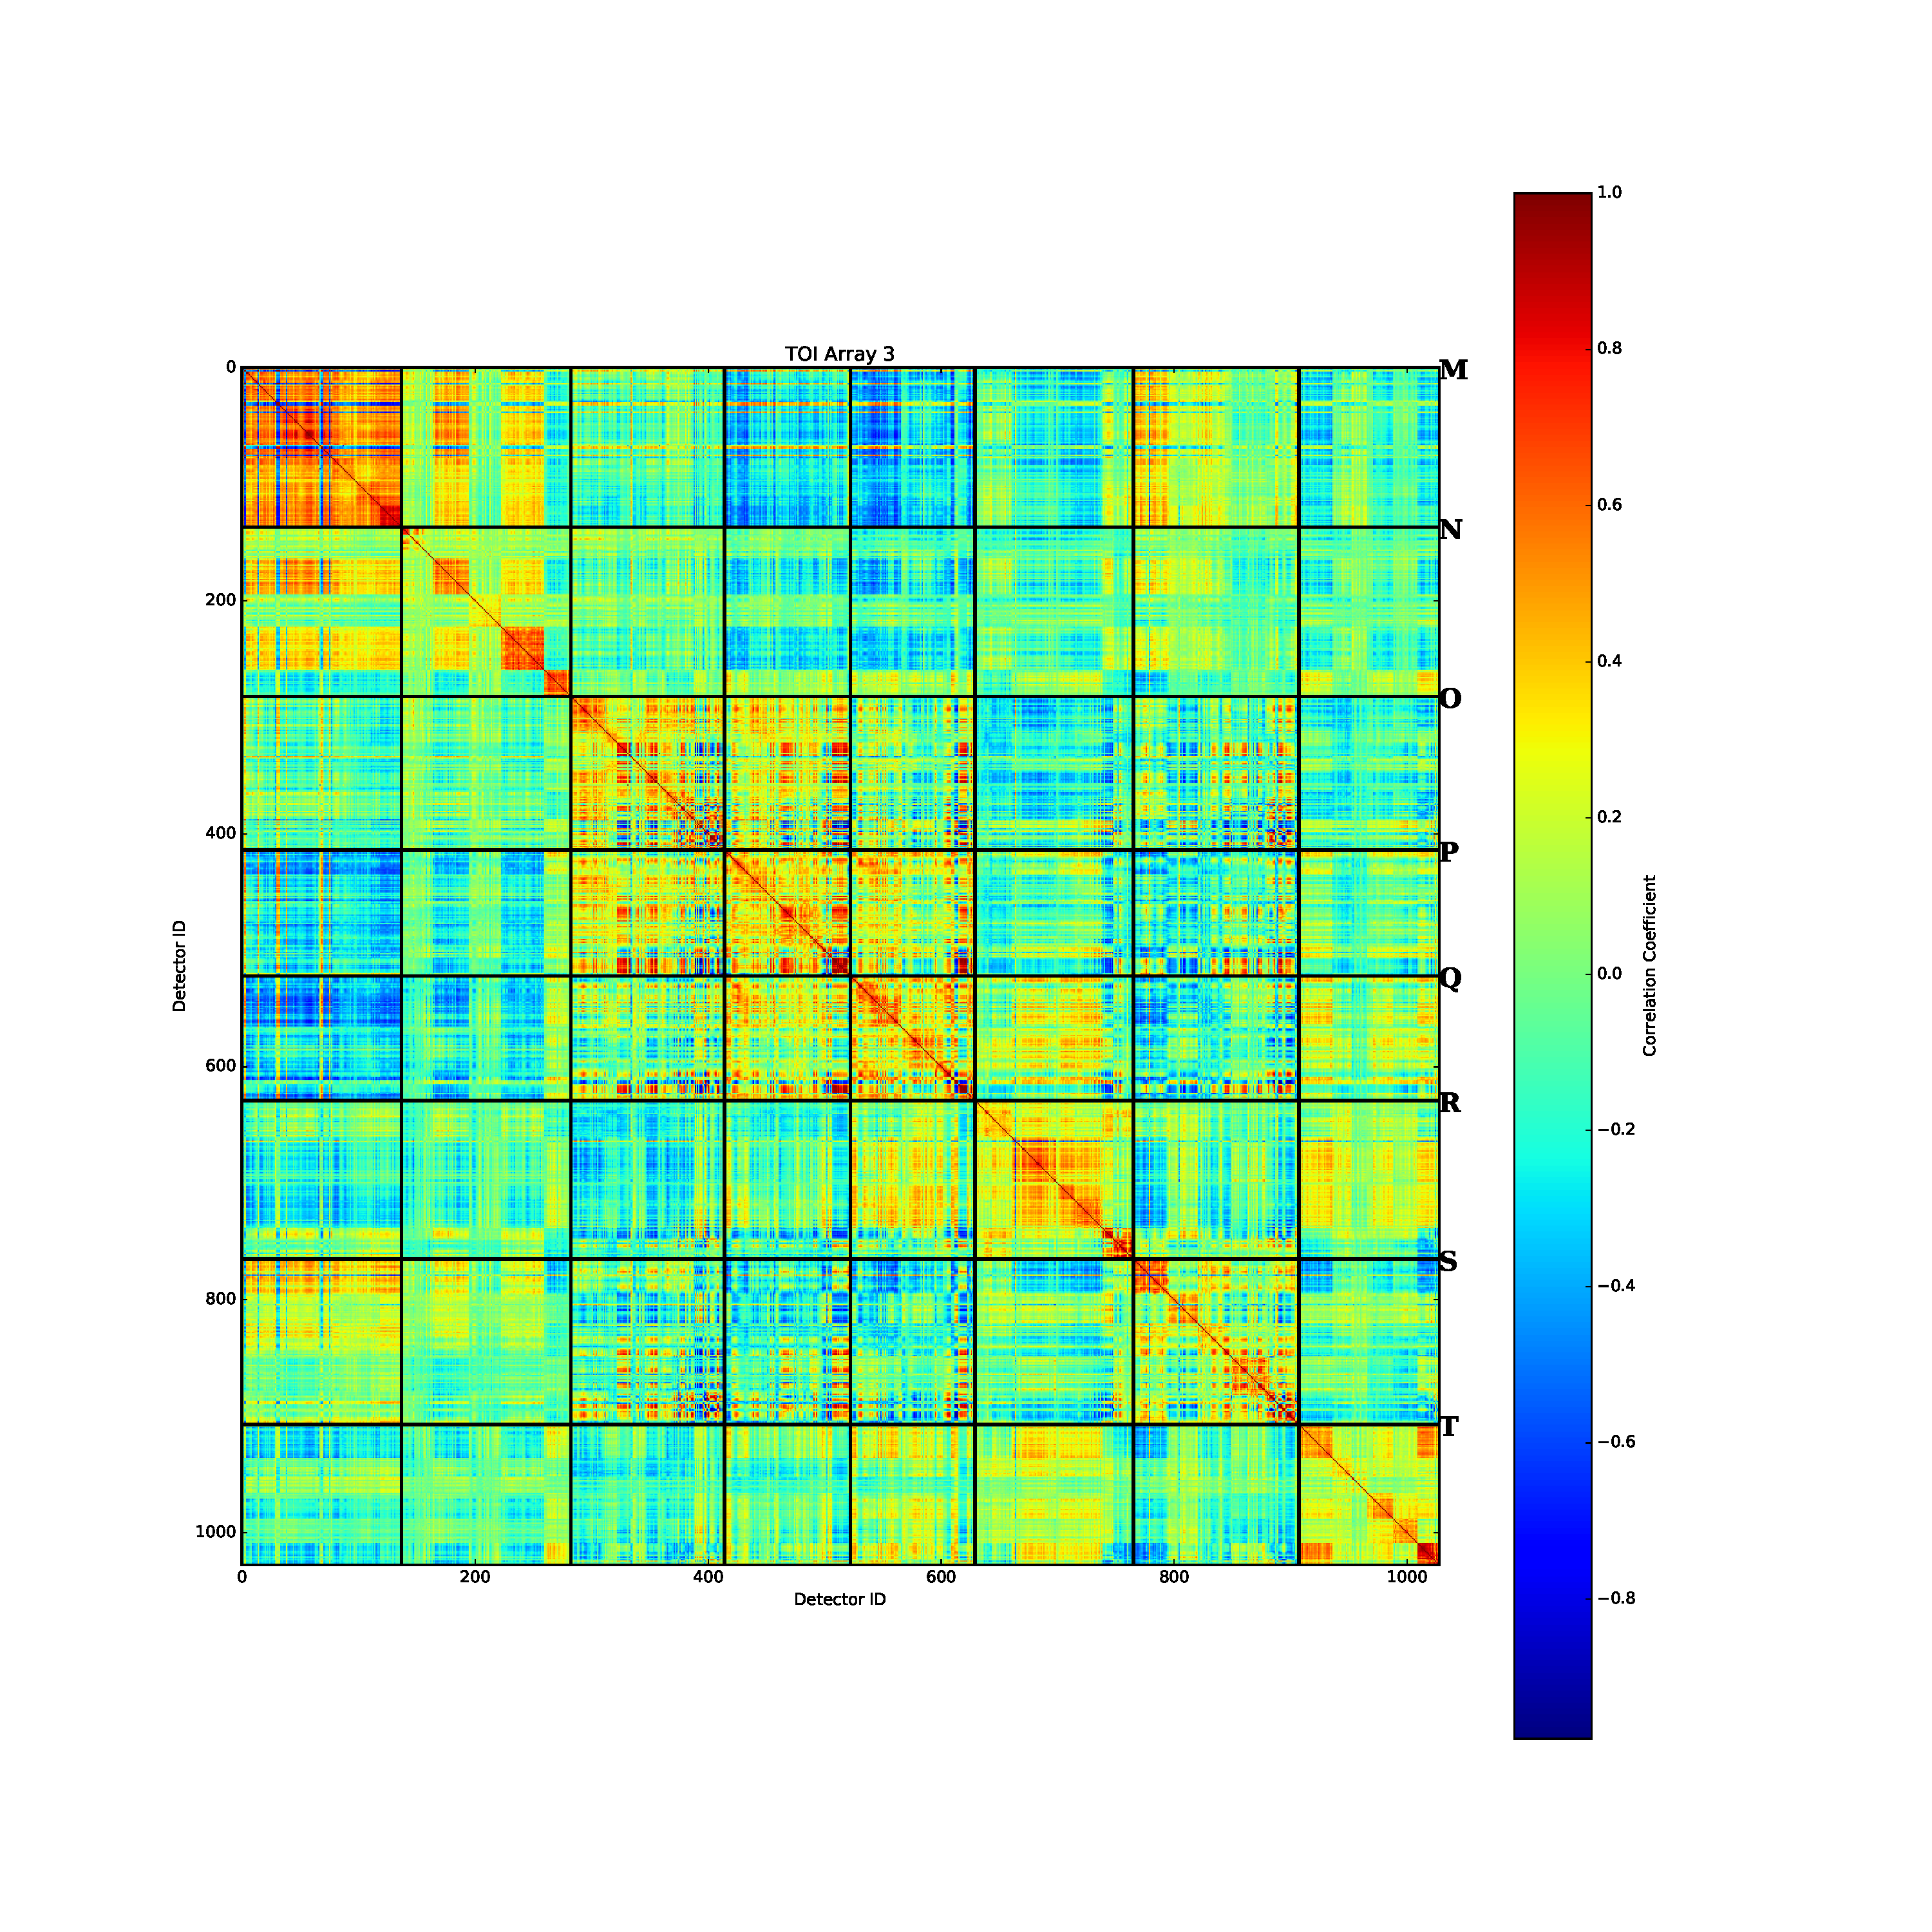
\includegraphics[width=0.3\textwidth]{Figures/DarkTests/corrmat_TOI_CM_array_3_20161213s72.pdf}
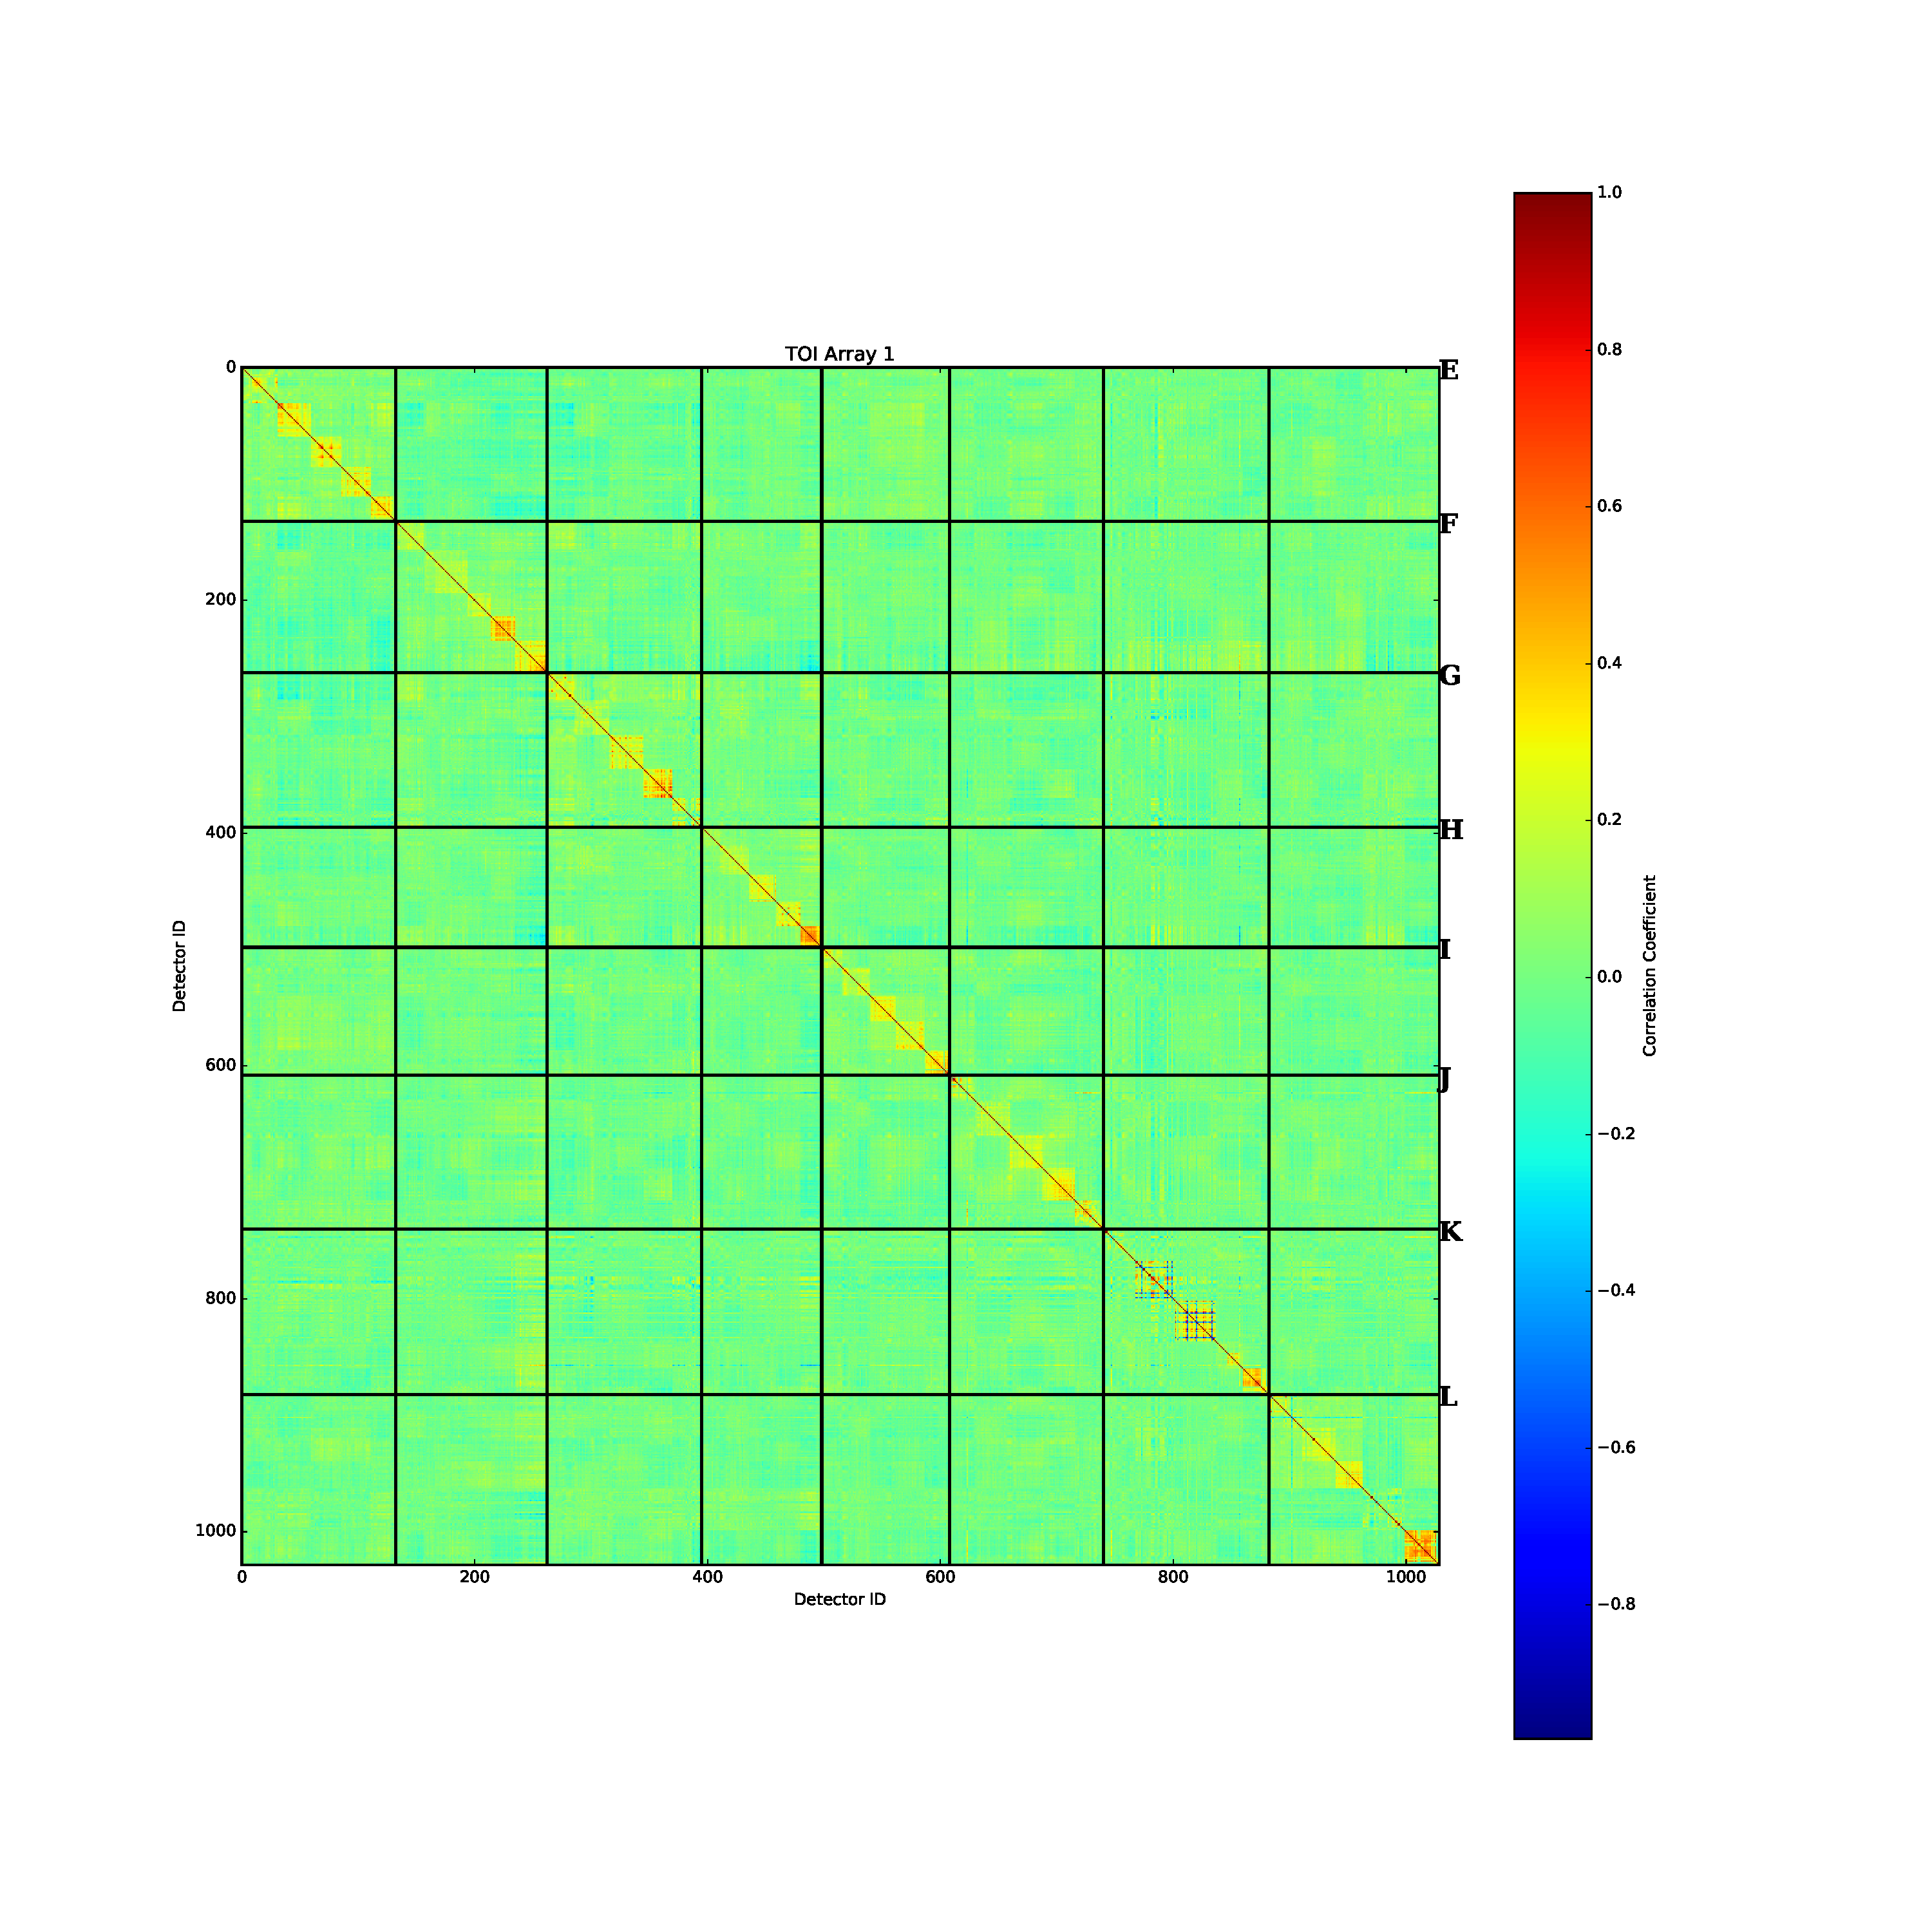
\includegraphics[width=0.3\textwidth]{Figures/DarkTests/corrmat_TOI_PCA_array_1_20161213s72.pdf}
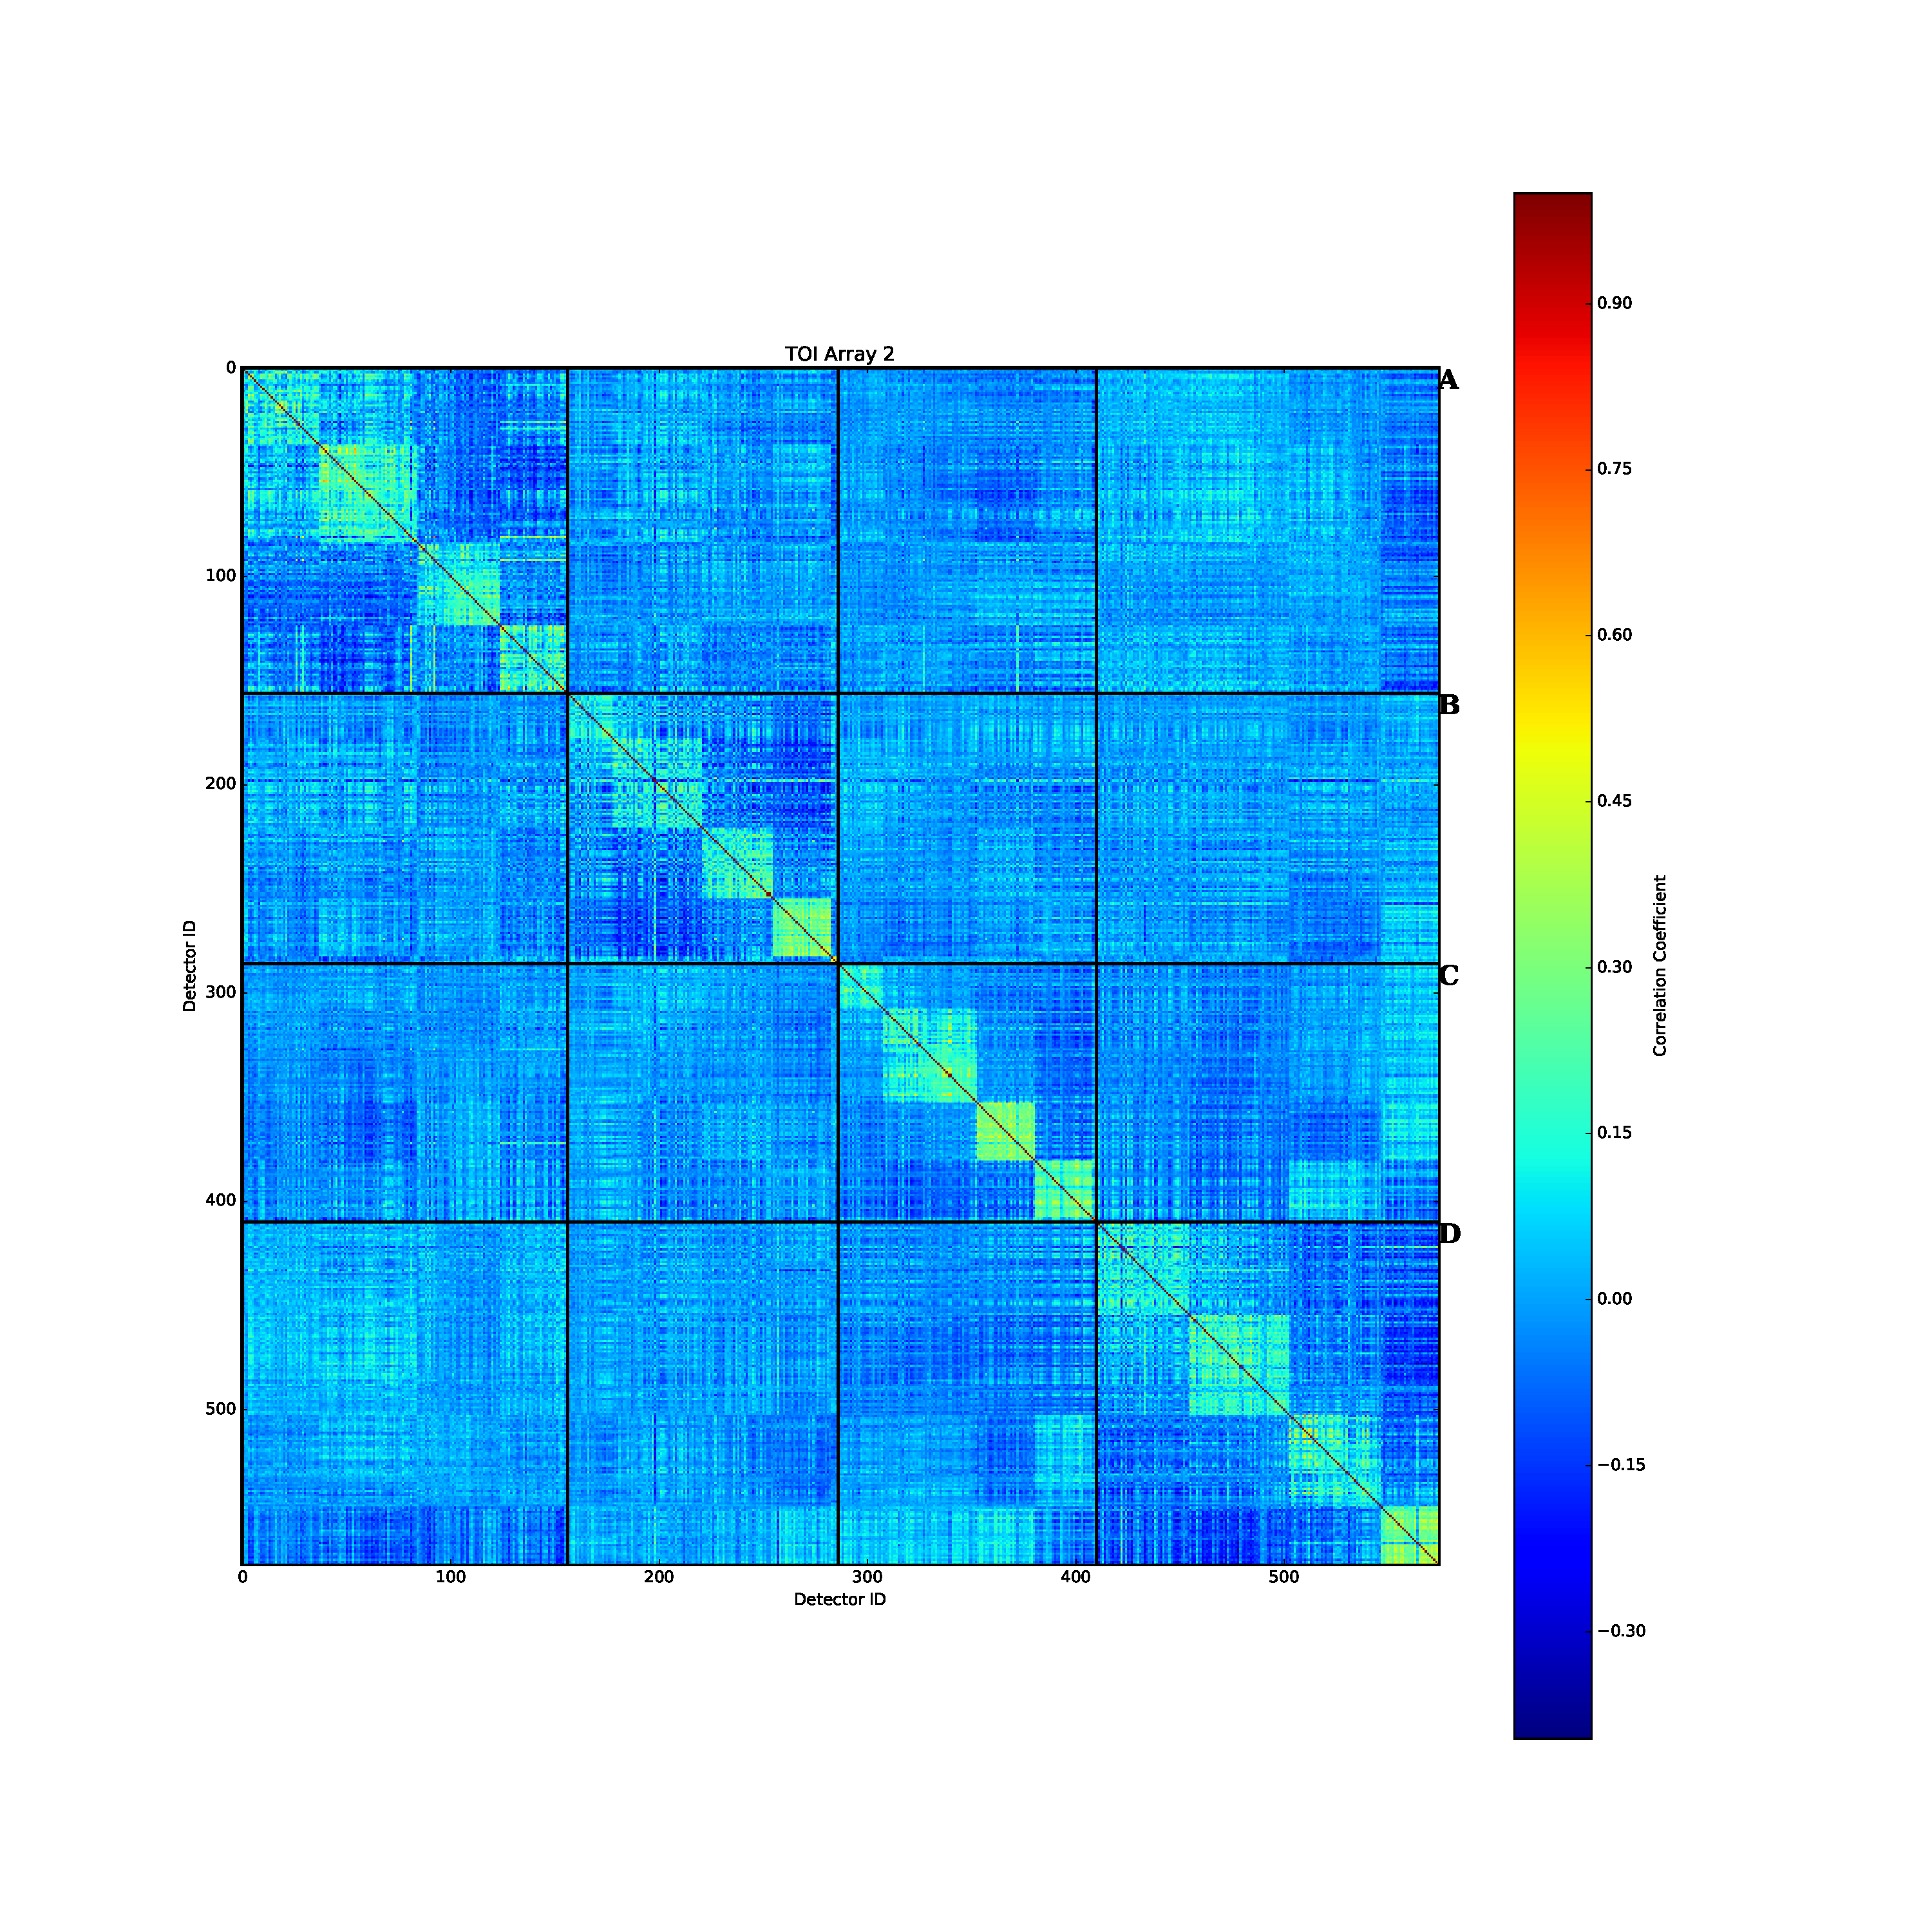
\includegraphics[width=0.3\textwidth]{Figures/DarkTests/corrmat_TOI_PCA_array_2_20161213s72.pdf}
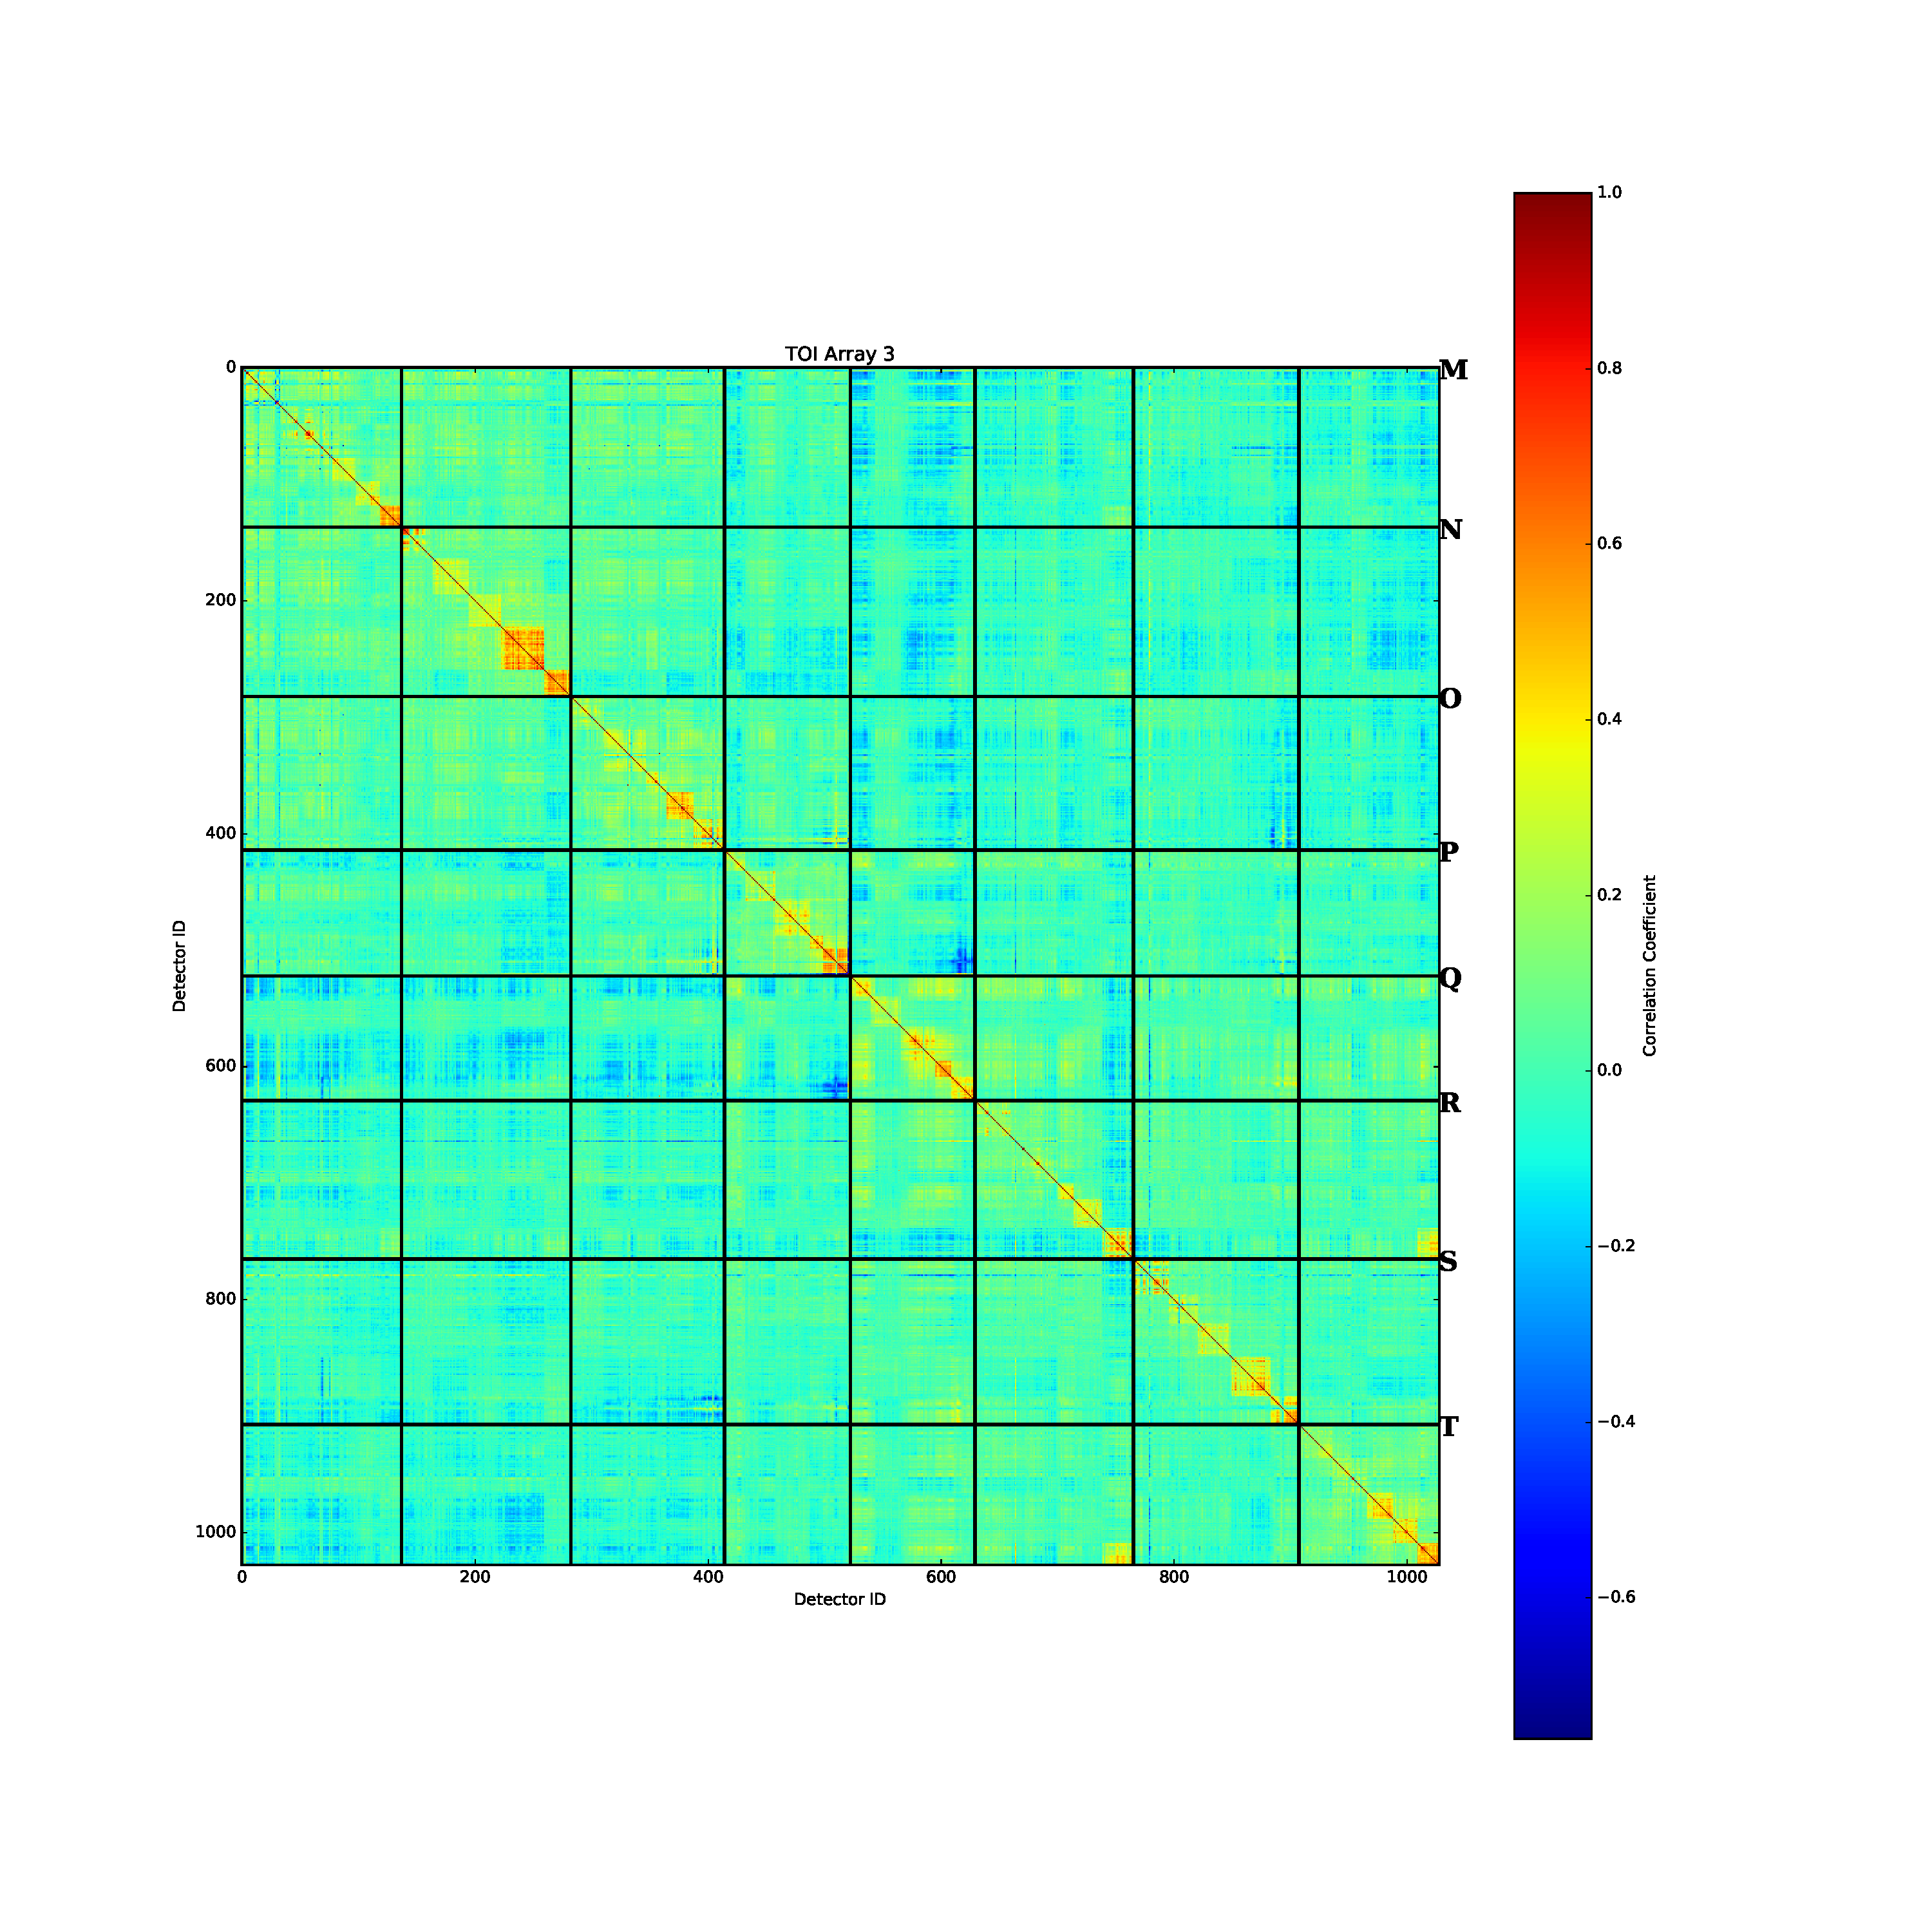
\includegraphics[width=0.3\textwidth]{Figures/DarkTests/corrmat_TOI_PCA_array_3_20161213s72.pdf}
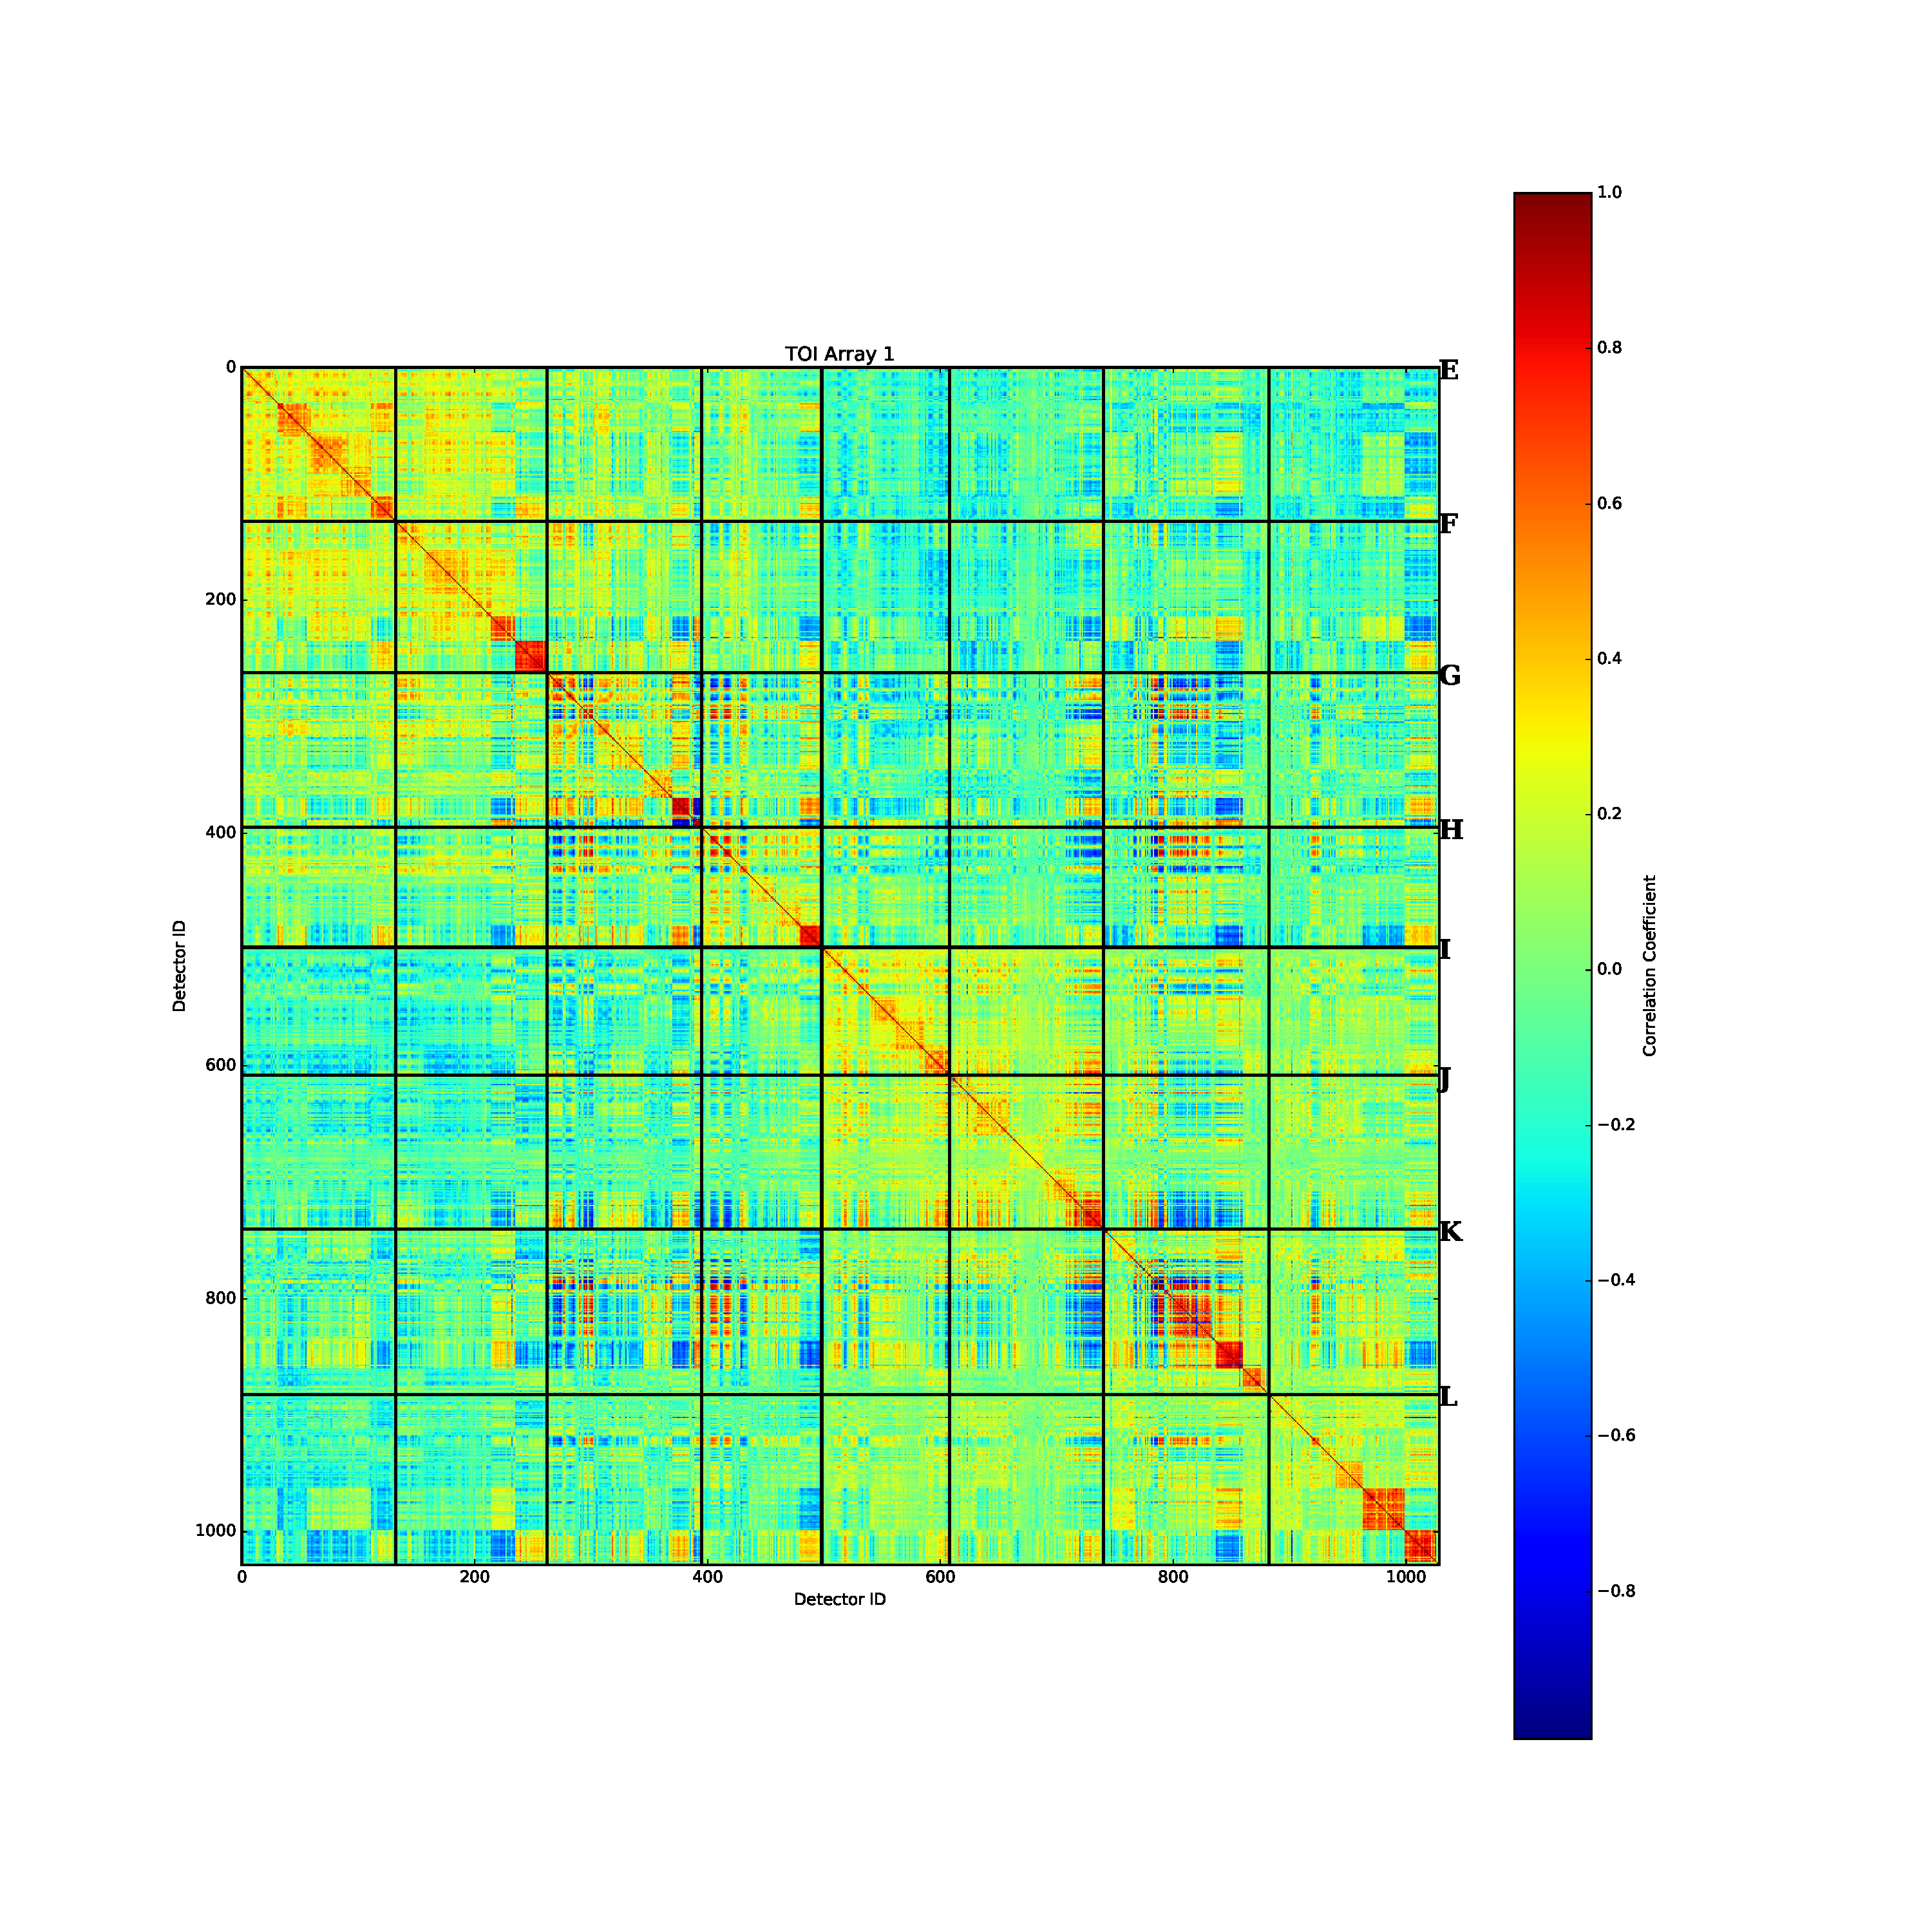
\includegraphics[width=0.3\textwidth]{Figures/DarkTests/corrmat_TOI_BC_array_1_20161213s72.pdf}
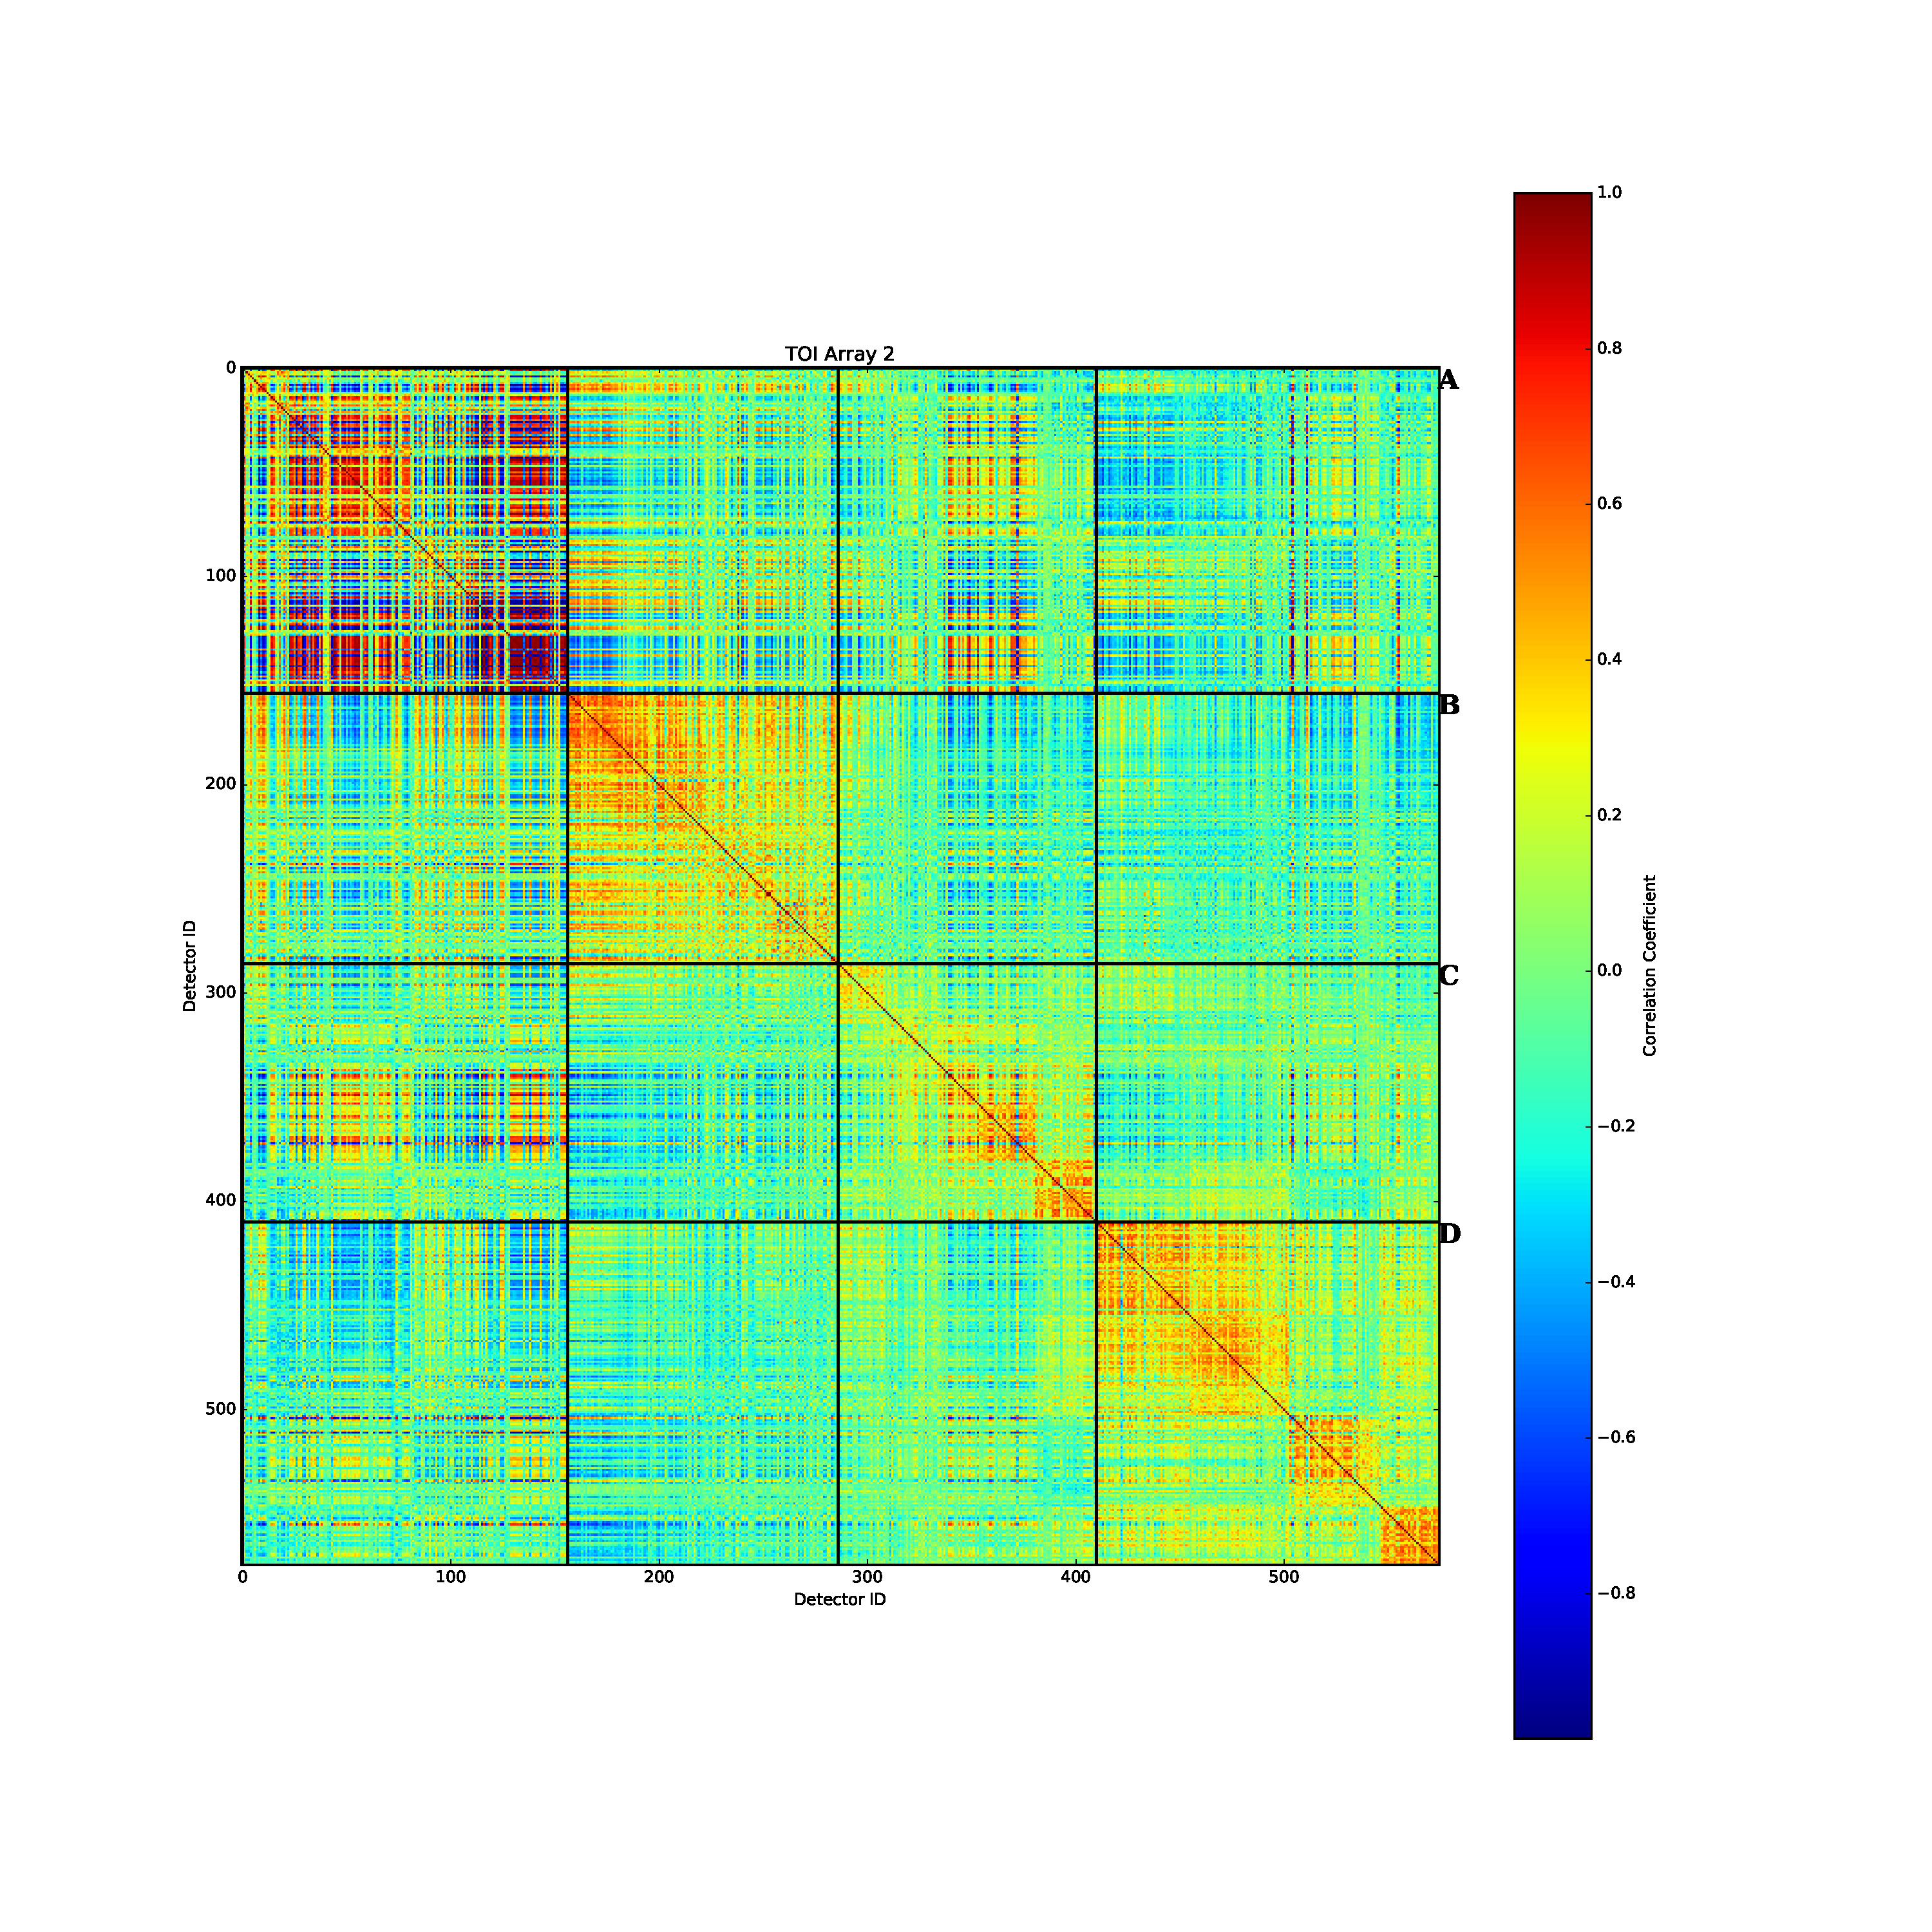
\includegraphics[width=0.3\textwidth]{Figures/DarkTests/corrmat_TOI_BC_array_2_20161213s72.pdf}
\includegraphics[width=0.3\textwidth]{Figures/DarkTests/corrmat_TOI_BC_array_3_20161213s72.pdf}
\end{center}
\caption{From left to right correlation matrices for the three NIKA2 arrays (A1, A2, and A3) for scan 20161213s72. From top to bottom we present the correlation of the raw data, after CM, PCA and BC decorrelations. \label{corrs72}}
\end{figure}


\begin{figure}[ht] % Inline image example
\begin{center}
\includegraphics[width=0.3\textwidth]{Figures/DarkTests/corrmat_TOI_array_1_20160504s97.pdf}
\includegraphics[width=0.3\textwidth]{Figures/DarkTests/corrmat_TOI_array_2_20160504s97.pdf}
\includegraphics[width=0.3\textwidth]{Figures/DarkTests/corrmat_TOI_array_3_20160504s97.pdf}
\includegraphics[width=0.3\textwidth]{Figures/DarkTests/corrmat_TOI_CM_array_1_20160504s97.pdf}
\includegraphics[width=0.3\textwidth]{Figures/DarkTests/corrmat_TOI_CM_array_2_20160504s97.pdf}
\includegraphics[width=0.3\textwidth]{Figures/DarkTests/corrmat_TOI_CM_array_3_20160504s97.pdf}
\includegraphics[width=0.3\textwidth]{Figures/DarkTests/corrmat_TOI_PCA_array_1_20160504s97.pdf}
\includegraphics[width=0.3\textwidth]{Figures/DarkTests/corrmat_TOI_PCA_array_2_20160504s97.pdf}
\includegraphics[width=0.3\textwidth]{Figures/DarkTests/corrmat_TOI_PCA_array_3_20160504s97.pdf}
\includegraphics[width=0.3\textwidth]{Figures/DarkTests/corrmat_TOI_BC_array_1_20160504s97.pdf}
\includegraphics[width=0.3\textwidth]{Figures/DarkTests/corrmat_TOI_BC_array_2_20160504s97.pdf}
\includegraphics[width=0.3\textwidth]{Figures/DarkTests/corrmat_TOI_BC_array_3_20160504s97.pdf}
\end{center}
\caption{From left to right correlation matrices for the three NIKA2 arrays (A1, A2, and A3) for scan 20160504s97. From top to bottom we present the correlation of the raw data, after CM, PCA and BC decorrelations. \label{corrs97}}
\end{figure}


\begin{figure}[ht] % Inline image example
\begin{center}
\includegraphics[width=0.3\textwidth]{Figures/DarkTests/corrmat_TOI_array_1_20160313s87.pdf}
\includegraphics[width=0.3\textwidth]{Figures/DarkTests/corrmat_TOI_array_2_20160313s87.pdf}
\includegraphics[width=0.3\textwidth]{Figures/DarkTests/corrmat_TOI_array_3_20160313s87.pdf}
\includegraphics[width=0.3\textwidth]{Figures/DarkTests/corrmat_TOI_CM_array_1_20160313s87.pdf}
\includegraphics[width=0.3\textwidth]{Figures/DarkTests/corrmat_TOI_CM_array_2_20160313s87.pdf}
\includegraphics[width=0.3\textwidth]{Figures/DarkTests/corrmat_TOI_CM_array_3_20160313s87.pdf}
\includegraphics[width=0.3\textwidth]{Figures/DarkTests/corrmat_TOI_PCA_array_1_20160313s87.pdf}
\includegraphics[width=0.3\textwidth]{Figures/DarkTests/corrmat_TOI_PCA_array_2_20160313s87.pdf}
\includegraphics[width=0.3\textwidth]{Figures/DarkTests/corrmat_TOI_PCA_array_3_20160313s87.pdf}
\includegraphics[width=0.3\textwidth]{Figures/DarkTests/corrmat_TOI_BC_array_1_20160313s87.pdf}
\includegraphics[width=0.3\textwidth]{Figures/DarkTests/corrmat_TOI_BC_array_2_20160313s87.pdf}
\includegraphics[width=0.3\textwidth]{Figures/DarkTests/corrmat_TOI_BC_array_3_20160313s87.pdf}
\end{center}
\caption{From left to right correlation matrices for the three NIKA2 arrays (A1, A2, and A3) for scan 20160313s87. From top to bottom we present the correlation of the raw data, after CM, PCA and BC decorrelations. \label{corrs87}}
\end{figure}


\subsection{RMS of the noise}

We present in Figure~\ref{rms299} the rms, in Hz, of the raw (dark blue) and decorrelated (CM, blue; PCA, red; and BC, cyan),data for the N2R7 dark test scan 21612101s299. We also show for comparison the rms of the data by extrapolating the median high frequency noise (PS, violet).
For the three arrays we observe that decorrelation reduces significantly the rms noise. The most efficient method is PCA as one would expect from previous results in the noise correlation matrix. \\

For each array the detectors are ordered by electronic box (separated by vertical black lines in the figure) and within each electronic box by increasing resonant frequency. We observe that median high frequency noise increases with increasing resonant frequency. A similar effect is observed for the PCA and BC rms noise but for some pathological detectors or electronic boxes. While in A2 the rms noise increases monotoneously with resonant frequency in arrays A1 and A3 we observe also observe fine structure within eash electronic box. For array A2, electronic box A, shows significantly larger raw rms. For array A1 box K seems to have a larger number of anomalous detectors than the other boxes. In array A3 all boxes seem to be equivalent to first order. Both in A1 and A3 we find complex structure within each box, which are not present in A2. \\

Similar results are found for scan 20161213s72 as shown in Figure~\ref{rms72}. However, we stress that the atmospheric emission shows significant contribution at high frequency (see PS) that is significantly reduced after decorrelation. \\

We have also computed the noise rms for the scans of N2R4 20160504s97 and 20160313s87. For arrays A1 and A3 the results are very similar to those for the N2R7 scans. However, we clearly observe that A2 is significantly worse in terms of misbehaving pixels.


%------------------------------------------------
\begin{figure}[ht] % Inline image example
\begin{center}
\includegraphics[scale=0.26]{Figures/DarkTests/rms_TOI_array_1_20161211s299.pdf} 
\includegraphics[scale=0.26]{Figures/DarkTests/rms_TOI_array_2_20161211s299.pdf} 
\includegraphics[scale=0.26]{Figures/DarkTests/rms_TOI_array_3_20161211s299.pdf} 
\end{center}
\caption{RMS noise for arrays 1,2,and 3 (top to bottom) for scan 20161211s299. The rms is computed for the raw data, and for the three decorrelation methods, CM. PCA and BC. The rms value for the level of white is also computed from the raw data power spectrum (PS). \label{rms299}}
\end{figure}


\begin{figure}[ht] % Inline image example
\begin{center}
\includegraphics[scale=0.26]{Figures/DarkTests/rms_TOI_array_1_20161213s72.pdf} 
\includegraphics[scale=0.26]{Figures/DarkTests/rms_TOI_array_2_20161213s72.pdf} 
\includegraphics[scale=0.26]{Figures/DarkTests/rms_TOI_array_3_20161213s72.pdf} 
\end{center}
\caption{Same as Figure~\ref{rms299} but for scan 20161213s72. \label{rms72}}
\end{figure}

\begin{figure}[ht] % Inline image example
\begin{center}
\includegraphics[scale=0.26]{Figures/DarkTests/rms_TOI_array_1_20160504s97.pdf} 
\includegraphics[scale=0.26]{Figures/DarkTests/rms_TOI_array_2_20160504s97.pdf} 
\includegraphics[scale=0.26]{Figures/DarkTests/rms_TOI_array_3_20160504s97.pdf} 
\end{center}
\caption{Same as Figure~\ref{rms299} but for scan 20160504s97. \label{rms97}}
\end{figure}



\begin{figure}[ht] % Inline image example
\begin{center}
\includegraphics[scale=0.26]{Figures/DarkTests/rms_TOI_array_1_20160313s87.pdf} 
\includegraphics[scale=0.26]{Figures/DarkTests/rms_TOI_array_2_20160313s87.pdf} 
\includegraphics[scale=0.26]{Figures/DarkTests/rms_TOI_array_3_20160313s87.pdf} 
\end{center}
\caption{Same as Figure~\ref{rms299} but for scan 20160313s87. \label{rms87}}
\end{figure}



\subsection{Discussion}

Using dark test measurements we have identified several noise components that require using complex decorrelation methods. Event in the case of multiple template decorrelation we find residual correlation between detectors that seems to be related to electronic subbands. Similar results are found when analyzing faint source scans. We find significant differences between N2R4 and N2R7 scans. \\

After decorralation using multiple template procedures we reduce significantly the rms of the noise. In the case of dark test it becomes of the level of the high frequency noise. For faint source scans we also diminish the high frequency noise, which is probably dominated by atmospheric emission. We find significant differences between the noise levels in A1 and A3, which might be explained by gain differences (to be verified). For some electronic boxes in A2 the rms noise is significantly larger than for the others. For the three arrays we find increasing noise with increasing resonant frequency withing each electronic box.This is probably related to the difference of gains between subbands in the electronics. Furthermore, we find in A1 and A3 extra low frequency structures in the rms which are not identified yet.



%----------------------------------------------------------------------------------------
%	SENSITIVITIES
%----------------------------------------------------------------------------------------
\section{Sensitivities}
\label{se:nefd}
%%
%%
%%      SECTION: SENSITIVITY
%%

\begin{figure}
\begin{center}
%\includegraphics[clip, angle=0, scale =
%  0.5]{Figures/NEFD_HLS091828_20170226s415_FXDC0C1_GaussPhot.png}
\includegraphics[clip, angle=0, scale = 0.5]{Figures/nefd_mpfit_HLS091828.eps}
\caption{Kids Xcalib with fixed fwhm 12.5 and 18.5, \hls.}
\label{fig:nefd_vs_t}
\end{center}
\end{figure}

{\bf The specs/goals ``NEFD on X \% of pixels'' should be understood as : we have
XX\% valid pixels, and with these pixels, we have an NEFD of YY. We should not
discard some fraction of our pixels and estimate an NEFD on this subset.}\\

\hls is moderately faint source, expected to be below 100~mJy at 1mm and
XX~mJy at 2mm {\bf check values in NIKA1 paper + use SED for predictions in
  NIKA2's bands}. This source was chosen for its flux and its availability during
Run9 for long integration. It has been observed for XX hours in total over three
nights.


\subsection{Observations}

As part of the NIKA2 Science Verification that took place in February 2017, we
observed an area of 185~arcmin$^2$, centered on \hls, (a lensed dusty galaxy at
z=5.24 \cite{combes2012}) during about 9~hours. The scans were 8x5~arcmin$^2$,
alternatively oriented in (ra,dec), (dec,ra), (az,el), (el,az). This leads to
the coverage presented on Fig.~\ref{fig:hls_cov} and effective integration times
on \hls\ of $\sim 2.4$\,hours at 2\,mm and $\sim 1.7$\,hours at 1.2\,mm (the
difference comes from the different density of detectors across the field of
view for the two bands). This allowed us to reach $1\sigma$ sensitivities of
about 0.3~mJy at 1.2\,mm and 0.1~mJy at 2\,mm on \hls. The integration time in a
map pixel $t_p$ of size $r\times r$~arcsec$^2$ is given by the number of hits in
this pixel $N_p$, divided by the sampling frequency $\nu$. This estimate is not
the time $t_{obs}$ that enters the definition of the NEFD and which is the time
spent by the matrix ``overall'' on the region where we give the
sensitivity. Indeed, we must account for the density of KIDs in the focal plane
compared to the map resolution : assume there are two KIDs per map pixel, then
$t_p = 2 t_{obs}$. A contrario, if the KIDs are sparsely distributed accross the
focal plane, some map pixels are empty while they are physically covered by the
FOV. Let's call $g$ the spacing between KIDs in arcsec in the FOV, we thus have:

\begin{eqnarray}
t_{obs} &=& \frac{t_p}{N_{kids\,per\,pix}} \nonumber\\
&=& \frac{t_p}{N_{kids}/N_{pix}} \nonumber\\
&=& \frac{t_p\pi R_{FOV}^2/r^2}{\pi R_{FOV}^2/g^2} \nonumber\\
&=&t_p g^2r^2
\end{eqnarray}

\begin{figure}[htbp]
\begin{center}
\includegraphics[clip, angle=0, scale = 0.30]{Figures/hls_sensit_1mm.eps}
\includegraphics[clip, angle=0, scale = 0.30]{Figures/hls_sensit_2mm.eps}
\caption{Sensitivity per beam in mJy at 1 and 2mm}
\label{fig:hls_cov}
\end{center}
\end{figure}


\subsection{Data processing}

The data were decorrelated using the {\tt common-monde-one-block} method
(cf.~\ref{se:cm1blck}), masking a disk of 60~arcsec radius centered \hls.  The
scans have been combined with standard inverse noise weighting. The noise in
each map pixel is derived from the rms of the background corrected by the square
root of the number of observations per pixel (N1). If the noise was perfectly
gaussian, the distribution of the map signal over this noise estimate (far from
the source) would be a normalized gaussian. In practice, this leads to gaussians
that 1.6 and 1.5 larger. We therefore increase our noise estimate (N1) by these
factors to derive our final estimates. Should the extra sources that pop up in
the field contribute to this estimate, they would only make our estimate more
conservative.

\subsection{NEFD Methods 1 and 2: deep integration}

These data can be used to derive the NEFD in several ways. One is to fit the
evolution of the uncertainty on the flux of the source $\sigma_\phi$ with the
integration time. Another one is to produce jackknife maps with the data and to
measure the uncertainty on the flux in the end, while estimating the time of
integration. Results are summarized in
Tab.~\ref{tab:nefd}. Fig.~\ref{fig:nefd_vs_t} shows the decrease of the
uncertainty on the measured flux at the center of the map as a function of
time. We either fit a power law or fix the power law to -0.5 and fit only the
amplitude. Uncertainties on these values have been estimated via a bootstrap
method: we randomize the scans and derive the standard deviation of the average
of $n$ scans for any $n$ between 1 and the total number of scans. This gives us
an estimate of the uncertainty on $\sigma_\phi$ for a time of integration
corresponding to $n$ scans. Strictly speaking, all the scans do not have the
exact same duration, but the difference is negligible here.

\begin{table}
\begin{tabular}{|l|l|l|l|l|}
\hline
Array & Free power law & Fixed power law $t^{-0.5}$ & Jackknife & Instrument \\
\hline
A1       & $47.9$ mJy.s$^{-0.54}$ & $37.9$ mJy.s$^{1/2}$ & 35.6 mJy.s$^{1/2}$ & $33.3$ (5) mJy.s$^{1/2}$\\
A2       & $5.2$  mJy.s$^{-0.51}$ & $4.8$  mJy.s$^{1/2}$ & 5.7  mJy.s$^{1/2}$ & $5.8$  (5) mJy.s$^{1/2}$\\
A3       & $38.9$ mJy.s$^{-0.54}$ & $30.6$ mJy.s$^{1/2}$ & 30.4 mJy.s$^{1/2}$ & $28.4$ (4) mJy.s$^{1/2}$\\
A1 \& A3 & $28.5$ mJy.s$^{-0.53}$ & $23.6$ mJy.s$^{1/2}$ & 22.4 mJy.s$^{1/2}$ & $21.1$ (3) mJy.s$^{1/2}$\\
\hline
\end{tabular}
\label{tab:nefd}
\caption{Noise integration with observation time and associated derivations of
  the NEFD. These values do not account for the extra {\color{red} \bf XXXX \%}
  uncertainty on absolute calibration.}
\end{table}
%       33.325263       5.2024647
%       28.397230       4.5723151
%       21.143376       4.1538804
%       5.7628233       3.3094792


\begin{figure}
\begin{center}
\includegraphics[clip, angle=0, scale =0.8]{Figures/NEFDIndScans/nefd_tau_run22.pdf}
\caption{Astronomer NEFD as a function of atmospheric background for the 1 (orange dots) and 2 (cyan dots) mm channels. We also show the expected NEFD evolution with atmospheric background (red and blue curves)}
\label{fig:nefdvsbackground}
\end{center}
\end{figure}

\subsection{NEFD Method 3: scan NEFD vs opacity and air mass}
\begin{figure}
\begin{center}
\includegraphics[clip, angle=0, scale =0.8]{Figures/NEFDIndScans/nefd_evol_run22.pdf}
\caption{Evolution of the measured instrument NEFD across scans for N2R9.}
\label{fig:nefdvsscans}
\end{center}
\end{figure}

\begin{figure}
\begin{center}
\includegraphics[clip, angle=0, scale =0.8]{Figures/NEFDIndScans/nefd_flux1mm_run22.pdf}
\caption{Measured instrument NEFD as a function of the flux of the source.}
\label{fig:nefdvsflux}
\end{center}
\end{figure}
\begin{figure}
\begin{center}
\includegraphics[clip, angle=0, scale =0.8]{Figures/NEFDIndScans/hist_nefd_ref_run22.pdf}
\caption{Histogram of the measured reference NEFD across the N2R9 for the 1 (right) and 2 (left) mm channels.}
\label{fig:nefdhist}
\end{center}
\end{figure}
 

In this section we investigate the astronomer NEFD as a function of the atmospheric opacity and air mass. Figure~\ref{fig:nefdvsbackground} shows the measured NEFD, which we refer to as astronomer NEFD, for the 1 and 2 mm as a function of the measured atmospheric background in terms of $\tau/sin(El)$. The atmospheric opacity was computed as discussed in Section~\ref{se:opacities}. We observe that the increase of the astronomer NEFD is in agreement with what we would expect for background dominated sensitivity. We observe however some significant deviations from the curve. To investigate this issue we also show in Figure~\ref{fig:nefdvsscans} the evolution of the background corrected NEFD, hereafter instrument NEFD, across the N2R9 campaign for arrays A1 (blue), A3 (green) and A2 (cyan), and for the combination of A1 and A3 (red). We globally obseve stable NEFD across the run, with A1 sensitivity being worse than for A3. We also show the measured instrument NEFD as a function of the flux of the source in the 1 mm channel in Figure~\ref{fig:nefdvsflux}. We observe that the observed deviations in the instrument NEFD correspond mainly to the large flux source scans. This is more obvious in Figure~\ref{fig:nefdhist} where we present the histogram of the measured NEFD for 2 mm of pwv and at a elevation of 60 degrees, hereafter, reference NEFD, for the 1 and 2 mm channels.





%----------------------------------------------------------------------------------------
%	SUMMARY
%----------------------------------------------------------------------------------------
\section{Summary of performance}



%----------------------------------------------------------------------------------------
%	BIBLIOGRAPHY
%----------------------------------------------------------------------------------------

\bibliographystyle{unsrt}

\bibliography{sample}

%----------------------------------------------------------------------------------------

\end{document}
